% Options for packages loaded elsewhere
%DIF LATEXDIFF DIFFERENCE FILE
%DIF DEL ms/LMAms_main_old.tex   Wed Nov  3 18:14:46 2021
%DIF ADD ms/LMAms_main.tex       Mon Nov 29 18:11:04 2021
\PassOptionsToPackage{unicode}{hyperref}
\PassOptionsToPackage{hyphens}{url}
%
\documentclass[
  12pt,
]{article}
%DIF 8a8
\usepackage{amsmath,amssymb} %DIF > 
%DIF -------
\usepackage{lmodern}
%DIF 9-11c10-11
%DIF < \usepackage{amssymb,amsmath}
%DIF < \usepackage{ifxetex,ifluatex}
%DIF < \ifnum 0\ifxetex 1\fi\ifluatex 1\fi=0 % if pdftex
%DIF -------
\usepackage{iftex} %DIF > 
\ifPDFTeX %DIF > 
%DIF -------
  \usepackage[T1]{fontenc}
  \usepackage[utf8]{inputenc}
  \usepackage{textcomp} % provide euro and other symbols
\else % if luatex or xetex
  \usepackage{unicode-math}
  \defaultfontfeatures{Scale=MatchLowercase}
  \defaultfontfeatures[\rmfamily]{Ligatures=TeX,Scale=1}
\fi
% Use upquote if available, for straight quotes in verbatim environments
\IfFileExists{upquote.sty}{\usepackage{upquote}}{}
\IfFileExists{microtype.sty}{% use microtype if available
  \usepackage[]{microtype}
  \UseMicrotypeSet[protrusion]{basicmath} % disable protrusion for tt fonts
}{}
\makeatletter
\@ifundefined{KOMAClassName}{% if non-KOMA class
  \IfFileExists{parskip.sty}{%
    \usepackage{parskip}
  }{% else
    \setlength{\parindent}{0pt}
    \setlength{\parskip}{6pt plus 2pt minus 1pt}}
}{% if KOMA class
  \KOMAoptions{parskip=half}}
\makeatother
\usepackage{xcolor}
\IfFileExists{xurl.sty}{\usepackage{xurl}}{} % add URL line breaks if available
\IfFileExists{bookmark.sty}{\usepackage{bookmark}}{\usepackage{hyperref}}
\hypersetup{
  hidelinks,
  pdfcreator={LaTeX via pandoc}}
\urlstyle{same} % disable monospaced font for URLs
\usepackage[margin=1in]{geometry}
%DIF 44c44-45
%DIF < \usepackage{longtable,booktabs}
%DIF -------
\usepackage{longtable,booktabs,array} %DIF > 
\usepackage{calc} % for calculating minipage widths %DIF > 
%DIF -------
% Correct order of tables after \paragraph or \subparagraph
\usepackage{etoolbox}
\makeatletter
\patchcmd\longtable{\par}{\if@noskipsec\mbox{}\fi\par}{}{}
\makeatother
% Allow footnotes in longtable head/foot
\IfFileExists{footnotehyper.sty}{\usepackage{footnotehyper}}{\usepackage{footnote}}
\makesavenoteenv{longtable}
\usepackage{graphicx}
\makeatletter
\def\maxwidth{\ifdim\Gin@nat@width>\linewidth\linewidth\else\Gin@nat@width\fi}
\def\maxheight{\ifdim\Gin@nat@height>\textheight\textheight\else\Gin@nat@height\fi}
\makeatother
% Scale images if necessary, so that they will not overflow the page
% margins by default, and it is still possible to overwrite the defaults
% using explicit options in \includegraphics[width, height, ...]{}
\setkeys{Gin}{width=\maxwidth,height=\maxheight,keepaspectratio}
% Set default figure placement to htbp
\makeatletter
\def\fps@figure{htbp}
\makeatother
\setlength{\emergencystretch}{3em} % prevent overfull lines
\providecommand{\tightlist}{%
  \setlength{\itemsep}{0pt}\setlength{\parskip}{0pt}}
\setcounter{secnumdepth}{-\maxdimen} % remove section numbering
%DIF 70a71-93
\newlength{\cslhangindent} %DIF > 
\setlength{\cslhangindent}{1.5em} %DIF > 
\newlength{\csllabelwidth} %DIF > 
\setlength{\csllabelwidth}{3em} %DIF > 
\newlength{\cslentryspacingunit} % times entry-spacing %DIF > 
\setlength{\cslentryspacingunit}{\parskip} %DIF > 
\newenvironment{CSLReferences}[2] % #1 hanging-ident, #2 entry spacing %DIF > 
 {% don't indent paragraphs %DIF > 
  \setlength{\parindent}{0pt} %DIF > 
  % turn on hanging indent if param 1 is 1 %DIF > 
  \ifodd #1 %DIF > 
  \let\oldpar\par %DIF > 
  \def\par{\hangindent=\cslhangindent\oldpar} %DIF > 
  \fi %DIF > 
  % set entry spacing %DIF > 
  \setlength{\parskip}{#2\cslentryspacingunit} %DIF > 
 }% %DIF > 
 {} %DIF > 
\usepackage{calc} %DIF > 
\newcommand{\CSLBlock}[1]{#1\hfill\break} %DIF > 
\newcommand{\CSLLeftMargin}[1]{\parbox[t]{\csllabelwidth}{#1}} %DIF > 
\newcommand{\CSLRightInline}[1]{\parbox[t]{\linewidth - \csllabelwidth}{#1}\break} %DIF > 
\newcommand{\CSLIndent}[1]{\hspace{\cslhangindent}#1} %DIF > 
%DIF -------
\usepackage{times}
\usepackage{setspace}
%DIF 72c96
%DIF < \doublespacing
%DIF -------
%\doublespacing %DIF > 
%DIF -------
\usepackage{lineno}
\linenumbers
\usepackage{amsmath}

\usepackage{booktabs}
\usepackage{longtable}
\usepackage{array}
\usepackage{multirow}
\usepackage{wrapfig}
\usepackage{float}
\usepackage{colortbl}
\usepackage{pdflscape}
\usepackage{tabu}
\usepackage{threeparttable}
\usepackage{threeparttablex}
\usepackage[normalem]{ulem}
\usepackage{makecell}
\usepackage{xcolor}
% \usepackage{array}
%DIF 92a116
%\usepackage[T1]{fontenc} %DIF > 
%DIF -------
\usepackage{booktabs}
\usepackage{longtable}
\usepackage{array}
\usepackage{multirow}
\usepackage{wrapfig}
\usepackage{float}
\usepackage{colortbl}
\usepackage{pdflscape}
\usepackage{tabu}
\usepackage{threeparttable}
\usepackage{threeparttablex}
\usepackage[normalem]{ulem}
\usepackage{makecell}
%DIF 105c130-131
%DIF < \ifluatex
%DIF -------
\usepackage{xcolor} %DIF > 
\ifLuaTeX %DIF > 
%DIF -------
  \usepackage{selnolig}  % disable illegal ligatures
\fi
%DIF 108-113d134
%DIF < \newlength{\cslhangindent}
%DIF < \setlength{\cslhangindent}{1.5em}
%DIF < \newenvironment{cslreferences}%
%DIF <   {\setlength{\parindent}{0pt}%
%DIF <   \everypar{\setlength{\hangindent}{\cslhangindent}}\ignorespaces}%
%DIF <   {\par}
%DIF -------

\author{}
\date{\vspace{-2.5em}}
%DIF PREAMBLE EXTENSION ADDED BY LATEXDIFF
%DIF UNDERLINE PREAMBLE %DIF PREAMBLE
\RequirePackage[normalem]{ulem} %DIF PREAMBLE
\RequirePackage{color}\definecolor{RED}{rgb}{1,0,0}\definecolor{BLUE}{rgb}{0,0,1} %DIF PREAMBLE
\providecommand{\DIFaddtex}[1]{{\protect\color{blue}\uwave{#1}}} %DIF PREAMBLE
\providecommand{\DIFdeltex}[1]{{\protect\color{red}\sout{#1}}}                      %DIF PREAMBLE
%DIF SAFE PREAMBLE %DIF PREAMBLE
\providecommand{\DIFaddbegin}{} %DIF PREAMBLE
\providecommand{\DIFaddend}{} %DIF PREAMBLE
\providecommand{\DIFdelbegin}{} %DIF PREAMBLE
\providecommand{\DIFdelend}{} %DIF PREAMBLE
\providecommand{\DIFmodbegin}{} %DIF PREAMBLE
\providecommand{\DIFmodend}{} %DIF PREAMBLE
%DIF FLOATSAFE PREAMBLE %DIF PREAMBLE
\providecommand{\DIFaddFL}[1]{\DIFadd{#1}} %DIF PREAMBLE
\providecommand{\DIFdelFL}[1]{\DIFdel{#1}} %DIF PREAMBLE
\providecommand{\DIFaddbeginFL}{} %DIF PREAMBLE
\providecommand{\DIFaddendFL}{} %DIF PREAMBLE
\providecommand{\DIFdelbeginFL}{} %DIF PREAMBLE
\providecommand{\DIFdelendFL}{} %DIF PREAMBLE
%DIF HYPERREF PREAMBLE %DIF PREAMBLE
\providecommand{\DIFadd}[1]{\texorpdfstring{\DIFaddtex{#1}}{#1}} %DIF PREAMBLE
\providecommand{\DIFdel}[1]{\texorpdfstring{\DIFdeltex{#1}}{}} %DIF PREAMBLE
\newcommand{\DIFscaledelfig}{0.5}
%DIF HIGHLIGHTGRAPHICS PREAMBLE %DIF PREAMBLE
\RequirePackage{settobox} %DIF PREAMBLE
\RequirePackage{letltxmacro} %DIF PREAMBLE
\newsavebox{\DIFdelgraphicsbox} %DIF PREAMBLE
\newlength{\DIFdelgraphicswidth} %DIF PREAMBLE
\newlength{\DIFdelgraphicsheight} %DIF PREAMBLE
% store original definition of \includegraphics %DIF PREAMBLE
\LetLtxMacro{\DIFOincludegraphics}{\includegraphics} %DIF PREAMBLE
\newcommand{\DIFaddincludegraphics}[2][]{{\color{blue}\fbox{\DIFOincludegraphics[#1]{#2}}}} %DIF PREAMBLE
\newcommand{\DIFdelincludegraphics}[2][]{% %DIF PREAMBLE
\sbox{\DIFdelgraphicsbox}{\DIFOincludegraphics[#1]{#2}}% %DIF PREAMBLE
\settoboxwidth{\DIFdelgraphicswidth}{\DIFdelgraphicsbox} %DIF PREAMBLE
\settoboxtotalheight{\DIFdelgraphicsheight}{\DIFdelgraphicsbox} %DIF PREAMBLE
\scalebox{\DIFscaledelfig}{% %DIF PREAMBLE
\parbox[b]{\DIFdelgraphicswidth}{\usebox{\DIFdelgraphicsbox}\\[-\baselineskip] \rule{\DIFdelgraphicswidth}{0em}}\llap{\resizebox{\DIFdelgraphicswidth}{\DIFdelgraphicsheight}{% %DIF PREAMBLE
\setlength{\unitlength}{\DIFdelgraphicswidth}% %DIF PREAMBLE
\begin{picture}(1,1)% %DIF PREAMBLE
\thicklines\linethickness{2pt} %DIF PREAMBLE
{\color[rgb]{1,0,0}\put(0,0){\framebox(1,1){}}}% %DIF PREAMBLE
{\color[rgb]{1,0,0}\put(0,0){\line( 1,1){1}}}% %DIF PREAMBLE
{\color[rgb]{1,0,0}\put(0,1){\line(1,-1){1}}}% %DIF PREAMBLE
\end{picture}% %DIF PREAMBLE
}\hspace*{3pt}}} %DIF PREAMBLE
} %DIF PREAMBLE
\LetLtxMacro{\DIFOaddbegin}{\DIFaddbegin} %DIF PREAMBLE
\LetLtxMacro{\DIFOaddend}{\DIFaddend} %DIF PREAMBLE
\LetLtxMacro{\DIFOdelbegin}{\DIFdelbegin} %DIF PREAMBLE
\LetLtxMacro{\DIFOdelend}{\DIFdelend} %DIF PREAMBLE
\DeclareRobustCommand{\DIFaddbegin}{\DIFOaddbegin \let\includegraphics\DIFaddincludegraphics} %DIF PREAMBLE
\DeclareRobustCommand{\DIFaddend}{\DIFOaddend \let\includegraphics\DIFOincludegraphics} %DIF PREAMBLE
\DeclareRobustCommand{\DIFdelbegin}{\DIFOdelbegin \let\includegraphics\DIFdelincludegraphics} %DIF PREAMBLE
\DeclareRobustCommand{\DIFdelend}{\DIFOaddend \let\includegraphics\DIFOincludegraphics} %DIF PREAMBLE
\LetLtxMacro{\DIFOaddbeginFL}{\DIFaddbeginFL} %DIF PREAMBLE
\LetLtxMacro{\DIFOaddendFL}{\DIFaddendFL} %DIF PREAMBLE
\LetLtxMacro{\DIFOdelbeginFL}{\DIFdelbeginFL} %DIF PREAMBLE
\LetLtxMacro{\DIFOdelendFL}{\DIFdelendFL} %DIF PREAMBLE
\DeclareRobustCommand{\DIFaddbeginFL}{\DIFOaddbeginFL \let\includegraphics\DIFaddincludegraphics} %DIF PREAMBLE
\DeclareRobustCommand{\DIFaddendFL}{\DIFOaddendFL \let\includegraphics\DIFOincludegraphics} %DIF PREAMBLE
\DeclareRobustCommand{\DIFdelbeginFL}{\DIFOdelbeginFL \let\includegraphics\DIFdelincludegraphics} %DIF PREAMBLE
\DeclareRobustCommand{\DIFdelendFL}{\DIFOaddendFL \let\includegraphics\DIFOincludegraphics} %DIF PREAMBLE
%DIF END PREAMBLE EXTENSION ADDED BY LATEXDIFF

\begin{document}

\textbf{Running title}: Metabolic and structural leaf mass

\textbf{Decomposing leaf mass into metabolic and structural components explains divergent patterns of trait variation within and among plant species}

Masatoshi Katabuchi\textsuperscript{1,2,\DIFdelbegin \DIFdel{3,7}\DIFdelend \DIFaddbegin \DIFadd{6}\DIFaddend }, Kaoru Kitajima\textsuperscript{\DIFaddbegin \DIFadd{2,}\DIFaddend 3,4\DIFdelbegin \DIFdel{,5}\DIFdelend }, S. Joseph Wright\textsuperscript{\DIFdelbegin \DIFdel{5}\DIFdelend \DIFaddbegin \DIFadd{4}\DIFaddend }, Sunshine A. Van Bael\textsuperscript{\DIFdelbegin \DIFdel{5}\DIFdelend \DIFaddbegin \DIFadd{4}\DIFaddend ,\DIFdelbegin \DIFdel{6}\DIFdelend \DIFaddbegin \DIFadd{5}\DIFaddend }, Jeanne L. D. Osnas\textsuperscript{\DIFdelbegin \DIFdel{3}\DIFdelend \DIFaddbegin \DIFadd{2}\DIFaddend } and Jeremy W. Lichstein\textsuperscript{\DIFdelbegin \DIFdel{3}\DIFdelend \DIFaddbegin \DIFadd{2}\DIFaddend }

\textsuperscript{1} Xishuangbanna Tropical Botanical Garden, Chinese Academy of Sciences, Menglun, Yunnan 666303 China

\textsuperscript{2} \DIFdelbegin \DIFdel{Center of Plant Ecology, Core Botanical Gardens, Chinese Academy of Sciences, Menglun, Yunnan 666303 China
}%DIFDELCMD < 

%DIFDELCMD < %%%
\DIFdel{\textsuperscript{3} }\DIFdelend Department of Biology, University of Florida, Gainesville, FL 32611, USA

\textsuperscript{\DIFdelbegin \DIFdel{4}\DIFdelend \DIFaddbegin \DIFadd{3}\DIFaddend } Graduate School of Agriculture, Kyoto University, Kitashirakawa Oiwake-Cho, Kyoto 606-8502 Japan

\textsuperscript{\DIFdelbegin \DIFdel{5}\DIFdelend \DIFaddbegin \DIFadd{4}\DIFaddend } Smithsonian Tropical Research Institute, 9100 Panama City Pl., Washington, DC 20521

\textsuperscript{\DIFdelbegin \DIFdel{6}\DIFdelend \DIFaddbegin \DIFadd{5}\DIFaddend } Department of Ecology and Evolutionary Biology, Tulane University, New Orleans, LA 70118 USA

\textsuperscript{\DIFdelbegin \DIFdel{7}\DIFdelend \DIFaddbegin \DIFadd{6}\DIFaddend } \textbf{Corresponding Author}: E-mail: \href{mailto:mattocci27@gmail.com}{\nolinkurl{mattocci27@gmail.com}}

\newpage

\hypertarget{abstract}{%
\section{Abstract}\label{abstract}}

\begin{itemize}
\item
  Across the global flora, photosynthetic and metabolic rates depend more strongly on leaf area than leaf mass.
  In contrast, intraspecific variation in these rates is strongly mass-dependent.
  These contrasting patterns suggest that the causes of variation in leaf mass per area (LMA) may be fundamentally different within vs.~among species.
\item
  We used statistical methods to decompose LMA into two conceptual components -- `metabolic LMAp (which determines photosynthetic capacity and metabolic rates, and also affects optimal leaf lifespan) and `structural' LMAs (which determines leaf toughness and potential leaf lifespan) using leaf trait data from tropical forest sites in Panama and a global leaf-trait database.
\item
  Statistically decomposing LMA into LMAp and LMAs provides improved predictions of trait variation (photosynthesis, respiration, and lifespan) across the global flora, and within and among tropical plant species in Panama.
  Our analysis shows that small scaling slope between metabolic leaf mass and photosynthetic rate, and similar variance in LMAp and in LMAs leads to area-proportionality of interspecific leaf traits.
  In contrast, intraspecific LMA variation is due to changes in LMAp, which explains why photosynthetic and metabolic traits are mass-dependent within species
\item
  Our results suggest that leaf trait variation is multi-dimensional and is not well-represented by the one-dimensional leaf economics spectrum.
\end{itemize}

\hypertarget{introduction}{%
\section{Introduction}\label{introduction}}

Leaf functional traits play an important role in ecological and physiological tradeoffs (\DIFdelbegin \DIFdel{Wright et al. }\DIFdelend \protect\DIFdelbegin %DIFDELCMD < \hyperlink{ref-Wright2004a}{2004}%%%
\DIFdel{, Onoda et al. }\DIFdelend \DIFaddbegin \hyperlink{ref-Wright2004a}{Wright et al. 2004}\DIFadd{, }\DIFaddend \protect\DIFdelbegin %DIFDELCMD < \hyperlink{ref-Onoda2017}{2017}%%%
\DIFdel{, Reich }\DIFdelend \DIFaddbegin \hyperlink{ref-Reich2014}{Reich 2014}\DIFadd{, }\DIFaddend \protect\DIFdelbegin %DIFDELCMD < \hyperlink{ref-Reich2014}{2014}%%%
\DIFdelend \DIFaddbegin \hyperlink{ref-Onoda2017}{Onoda et al. 2017}\DIFaddend ) and in carbon and nutrient cycling (\DIFaddbegin \protect\hyperlink{ref-Tcherkez2017}{Tcherkez et al. 2017}\DIFadd{, }\DIFaddend e.g., \DIFdelbegin \DIFdel{Huntingford et al. }\DIFdelend \protect\DIFdelbegin %DIFDELCMD < \hyperlink{ref-Huntingford2017}{2017}%%%
\DIFdel{, Tcherkez et al. }%DIFDELCMD < \protect\hyperlink{ref-Tcherkez2017}{2017}%%%
\DIFdelend \DIFaddbegin \hyperlink{ref-Huntingford2017}{Huntingford et al. 2017}\DIFaddend ).
Thus, understanding the causes and consequences of leaf trait variation is an important goal in ecology, plant physiology, and biogeochemistry (references).
Different leaf assemblages exhibit markedly different patterns of trait variation.
For example, across global species, whole-leaf values of traits related to photosynthesis and metabolism (e.g., the photosynthetic capacity, respiration rate, or nutrient content of an entire leaf) tend to increase with leaf area, but not leaf mass per area (LMA; Osnas et al. (\protect\hyperlink{ref-Osnas2013}{2013})).
In contrast, within species, these same whole-leaf trait values tend to increase with LMA from shade to full sunlight (\DIFdelbegin \DIFdel{Osada et al. }\DIFdelend \protect\DIFdelbegin %DIFDELCMD < \hyperlink{ref-Osada2001}{2001}%%%
\DIFdel{, Osnas et al. }\DIFdelend \DIFaddbegin \hyperlink{ref-Osada2001}{Osada et al. 2001}\DIFadd{, }\DIFaddend \protect\DIFdelbegin %DIFDELCMD < \hyperlink{ref-Osnas2013}{2013}%%%
\DIFdelend \DIFaddbegin \hyperlink{ref-Osnas2018}{Osnas et al. 2018}\DIFaddend ).
Functional groups (e.g., deciduous vs.~evergreen angiosperms) also differ from each other in terms of how \DIFdelbegin \DIFdel{interspecific trait variation depends }\DIFdelend \DIFaddbegin \DIFadd{photosynthetic and metabolic traits variation depend }\DIFaddend on leaf mass and area (\DIFdelbegin \DIFdel{Osnas et al. }\DIFdelend \protect\DIFdelbegin %DIFDELCMD < \hyperlink{ref-Osnas2018}{2018}%%%
\DIFdelend \DIFaddbegin \hyperlink{ref-Osnas2018}{Osnas et al. 2018}\DIFaddend ).
These divergent patterns suggest the presence of multiple drivers of trait variation.

Strong interspecific correlations among LMA, leaf lifespan (LL), and mass-normalized leaf traits related to photosynthesis and metabolism have been interpreted as evidence for a single dominant axis of leaf functional variation (\DIFdelbegin \DIFdel{Wright et al. }\DIFdelend \protect\DIFdelbegin %DIFDELCMD < \hyperlink{ref-Wright2004a}{2004}%%%
\DIFdelend \DIFaddbegin \hyperlink{ref-Wright2004a}{Wright et al. 2004}\DIFaddend ).
However, \DIFdelbegin \DIFdel{several studies suggest that }\DIFdelend \DIFaddbegin \DIFadd{the interpretation of }\DIFaddend these strong correlations\DIFaddbegin \DIFadd{, which }\DIFaddend result from mass-normalization of area-dependent traits (\DIFdelbegin \DIFdel{Lloyd et al. }\DIFdelend \protect\DIFdelbegin %DIFDELCMD < \hyperlink{ref-Lloyd2013}{2013}%%%
\DIFdel{, Osnas et al. }\DIFdelend \DIFaddbegin \hyperlink{ref-Lloyd2013}{Lloyd et al. 2013}\DIFadd{, }\DIFaddend \protect\DIFdelbegin %DIFDELCMD < \hyperlink{ref-Osnas2013}{2013}%%%
\DIFdel{).
Thus, although }\DIFdelend \DIFaddbegin \hyperlink{ref-Osnas2013}{Osnas et al. 2013}\DIFadd{), is controversial.
On the one hand, }\DIFaddend mass-normalization \DIFdelbegin \DIFdel{and the LES can be justified from economic principles (Westoby et al.
}\DIFdelend \DIFaddbegin \DIFadd{has been justified based on economic principles alone (}\DIFaddend \protect\DIFdelbegin %DIFDELCMD < \hyperlink{ref-Westoby2013}{2013}%%%
\DIFdel{), the }\DIFdelend \DIFaddbegin \hyperlink{ref-Westoby2013}{Westoby et al. 2013}\DIFadd{), because leaf mass provides a simple index of investment that underlies the leaf economics spectrum (LES), ranging from cheap, low-LMA leaves with a fast rate of return per-unit investment to expensive, high-LMA leaves with a slow rate of return (}\protect\hyperlink{ref-Wright2004a}{Wright et al. 2004}\DIFadd{).
On the other hand, because the lifetime return on investment depends on LL (}\protect\hyperlink{ref-Westoby2000}{Westoby et al. 2000}\DIFadd{, }\protect\hyperlink{ref-Falster2012}{Falster et al. 2012}\DIFadd{), it has been argued that annualized construction costs (or mass/LL) should be used as a normalizer in leaf economics analyses (}\protect\hyperlink{ref-Osnas2013}{Osnas et al. 2013}\DIFadd{).
In global analyses, normalizing leaf traits by mass/LL yields similarly weak correlations as area-normalization, because leaf area is roughly proportional to mass/LL across global species (}\protect\hyperlink{ref-Osnas2013}{Osnas et al. 2013}\DIFadd{).
Area-dependence of metabolic traits and the inconsistent correlation strengths obtained from different normalizers (}\protect\hyperlink{ref-Lloyd2013}{Lloyd et al. 2013}\DIFadd{, }\protect\hyperlink{ref-Osnas2013}{Osnas et al. 2013}\DIFadd{) do not invalidate mass-normalization or the LES (}\protect\hyperlink{ref-Westoby2013}{Westoby et al. 2013}\DIFadd{)
These considerations do, however, lead us to question the }\DIFaddend evidence for a single dominant axis \DIFdelbegin \DIFdel{is controversial}\DIFdelend \DIFaddbegin \DIFadd{of leaf functional diversity, which has important implications for how trait variation is represented in vegetation models (}\protect\hyperlink{ref-Bonan2002}{Bonan et al. 2002}\DIFadd{, }\protect\hyperlink{ref-Sakschewski2016}{Sakschewski et al. 2016}\DIFadd{)}\DIFaddend .

To understand why the same data can be interpreted as either supporting or opposing the existence of a single dominant axis of leaf trait variation, consider the conceptual model proposed by Osnas et al. (\protect\hyperlink{ref-Osnas2018}{2018}), in which LMA is comprised of two additive components:
\DIFdelbegin \DIFdel{structural leaf }\DIFdelend \DIFaddbegin \DIFadd{photosynthetic LMA (LMAp) -- the }\DIFaddend mass per area \DIFaddbegin \DIFadd{of chloroplasts and other metabolically active leaf components that contribute directly to photosynthesis -- and structural LMA }\DIFaddend (LMAs) \DIFdelbegin \DIFdel{and photosynthetic (hereafter `metabolic') leaf }\DIFdelend \DIFaddbegin \DIFadd{-- the }\DIFaddend mass per area \DIFdelbegin \DIFdel{(LMAp).
Suppose that }\DIFdelend \DIFaddbegin \DIFadd{of structural leaf components that contribute to toughness and durability (}\protect\hyperlink{ref-Kitajima2012}{Kitajima et al. 2012}\DIFadd{, }\protect\hyperlink{ref-Kitajima2016}{2016}\DIFadd{, }\protect\hyperlink{ref-Onoda2017}{Onoda et al. 2017}\DIFadd{).
Consider the scenario where }\DIFaddend these two LMA components are independent axes of functional variation\DIFaddbegin \DIFadd{, so that LMAp and LMAs are uncorrelated across species }\DIFaddend (Fig.\DIFaddbegin \DIFadd{~}\DIFaddend \ref{fig:Hplt}a).
These two independent axes can be translated into either a two-dimensional trait space (if metabolic traits are area-normalized; Fig.\DIFaddbegin \DIFadd{~}\DIFaddend \ref{fig:Hplt}b) or a one-dimensional trait space (if metabolic traits are mass-normalized; Fig.\DIFaddbegin \DIFadd{~}\DIFaddend \ref{fig:Hplt}c).
\DIFdelbegin \DIFdel{Essentially, mass-normalization can collapse one of the functional dimensions, because leaves that differ substantially in their metabolic investment per-unit area can have similar values of mass-normalized metabolic traits (Fig.
\ref{fig:Hplt}bc).
}\DIFdelend \DIFaddbegin \DIFadd{While both Fig.~\ref{fig:Hplt}b and Fig.~\ref{fig:Hplt}c are both `correct' representations of the same data, they lead to different perceptions about the dimensionality of leaf functional variation.
If LMAp, LMAs, and/or other axes are largely independent and have distinct functional consequences, then it would not be possible to accurately represent functional variation with a single axis.
}\DIFaddend 

The hypothetical example in Fig.\DIFaddbegin \DIFadd{~}\DIFaddend \ref{fig:Hplt} shows how mass-normalization can, in principle, make a two-dimensional trait space appear one-dimensional, but this example does not resolve the dimensionality of functional variation in real leaf assemblages.
One way to better understand the dimensionality of leaf trait variation is to compare models with different numbers of dimensions, and to ask if models with multiple dimensions provide improved statistical fits and conceptual insights compared to a single axis.
For example, the two-dimensional `LMAp + LMAs' model proposed by Osnas et al. (\protect\hyperlink{ref-Osnas2018}{2018}) could be compared to a one-dimensional LMA model in terms of their capacities to explain variation in other traits.
\DIFdelbegin \DIFdel{Doing so would require }\DIFdelend \DIFaddbegin \DIFadd{However, }\DIFaddend implementing the `LMAp + LMAs' model \DIFdelbegin \DIFdel{in a quantitative framework.
Implementing this model }\DIFdelend is challenging, because although certain leaf mass components can be neatly classified as `metabolic' or `structural' (\DIFdelbegin \DIFdel{Poorter et al. }\DIFdelend \protect\DIFdelbegin %DIFDELCMD < \hyperlink{ref-Poorter2009}{2009}%%%
\DIFdel{, Osnas et al. }\DIFdelend \DIFaddbegin \hyperlink{ref-Poorter2009}{Poorter et al. 2009}\DIFadd{, }\DIFaddend \protect\DIFdelbegin %DIFDELCMD < \hyperlink{ref-Osnas2018}{2018}%%%
\DIFdelend \DIFaddbegin \hyperlink{ref-Osnas2018}{Osnas et al. 2018}\DIFaddend ), other leaf mass components cannot.
For example, thick cell walls contribute to structural toughness (\DIFdelbegin \DIFdel{Onoda et al. }\DIFdelend \protect\DIFdelbegin %DIFDELCMD < \hyperlink{ref-Onoda2015}{2015}%%%
\DIFdelend \DIFaddbegin \hyperlink{ref-Onoda2015}{Onoda et al. 2015}\DIFaddend ), but at least some cell wall mass is required for the biomechanical support that enables photosynthesis.
\DIFdelbegin \DIFdel{One way forward is to use statistical methods to partition }\DIFdelend \DIFaddbegin \DIFadd{Thus, partitioning }\DIFaddend LMA into different \DIFdelbegin \DIFdel{components, rather than relying on direct measurements of morphological components (e.
g., John et al. (}%DIFDELCMD < \protect\hyperlink{ref-John2017}{2017}%%%
\DIFdel{)).
}\DIFdelend \DIFaddbegin \DIFadd{functional components requires novel empirical or modeling approaches.
}\DIFaddend 

In this paper, we present a statistical modeling framework to partition LMA into metabolic and structural components: LMAp and LMAs.
We develop and test \DIFdelbegin \DIFdel{the }\DIFdelend \DIFaddbegin \DIFadd{this two-dimensional }\DIFaddend model using leaf trait data from two tropical forest sites (sun and shade leaves from wet and dry sites in Panama) and the GLOPNET global leaf traits database (\DIFdelbegin \DIFdel{Wright et al. }\DIFdelend \protect\DIFdelbegin %DIFDELCMD < \hyperlink{ref-Wright2004a}{2004}%%%
\DIFdelend \DIFaddbegin \hyperlink{ref-Wright2004a}{Wright et al. 2004}\DIFaddend ).
We use the model to address the following questions: (1) How does variation in LMA components related with mass and area proportionality of leaf traits? (2) Do LMAp and LMAs differ between evergreen and deciduous species, and between sun and shade leaves? and (3) How are measurable leaf photosynthetic and structural traits (e.g., concentrations of nitrogen and cellulose) related to LMAp and LMAs?

\hypertarget{material-and-methods}{%
\section{Material and Methods}\label{material-and-methods}}

\DIFdelbegin %DIFDELCMD < \hypertarget{model-overview}{%
%DIFDELCMD < \subsection{Model overview}\label{model-overview}}
%DIFDELCMD < %%%
\DIFdelend \DIFaddbegin \hypertarget{overview}{%
\subsection{Overview}\label{overview}}
\DIFaddend 

We \DIFdelbegin \DIFdel{developed a statistical modeling framework to partition LMAinto additive LMAs and LMAp components (see below and Supplement SX).
For sample }\emph{\DIFdel{i}} %DIFAUXCMD
\DIFdel{(e.g.
, sun or shade leaves of a given species; see Datasets below) , we partition LMA \textsubscript{\emph{i}} into LMAp\textsubscript{\emph{i}} = }\emph{\DIFdel{f\textsubscript{i}}} %DIFAUXCMD
\DIFdel{× LMA \textsubscript{\emph{i}} and LMAs\textsubscript{\emph{i}} = (1 }\DIFdelend \DIFaddbegin \DIFadd{considered multiple approaches to modeling datasets that include observations of leaf mass per area (LMA), leaf lifespan (LL), net photosynthetic capacity (A), and dark respiration rate (R).
These traits comprise four of the six traits in the global leaf economics spectrum (LES) analysis of Wright et al.~(2004).
For simplicity, we did not include the other two LES traits }\DIFaddend -- \DIFaddbegin \DIFadd{leaf nitrogen (N) and phosphorus (P) concentrations -- in our modeling framework, but we did explore relationships between our model predictions and observed leaf N and P.
We considered a simple one-dimensional model that predicts LL, A, and R from LMA alone, as well as two-dimensional models that predict LL, A, and R from two additive LMA components: structural and metabolic leaf mass per area (LMAs and LMAp, respectively).
We formulate the models in terms of area-normalized A and R (}\DIFaddend \emph{\DIFdelbegin \DIFdel{f\textsubscript{i}}%DIFDELCMD < \MBLOCKRIGHTBRACE%%%
\DIFdel{)× LMA \textsubscript{\emph{i}} by estimating a latent variable }\emph{\DIFdel{f\textsubscript{i}}}%DIFAUXCMD
\DIFdel{.
The latent variables }\emph{\DIFdel{f\textsubscript{i}}} %DIFAUXCMD
\DIFdel{are not directly observed, but they can be constrained by available data using Bayesian methods (Bishop }%DIFDELCMD < \protect\hyperlink{ref-Bishop2006}{2006}%%%
\DIFdel{, Gelman and Hill }%DIFDELCMD < \protect\hyperlink{ref-Gelman2006}{2006}%%%
\DIFdel{).For example, we would expect high values of }\emph{\DIFdel{f\textsubscript{i}}} %DIFAUXCMD
\DIFdel{(high LMAp\textsubscript{\emph{i}})for leaves with high }\emph{\DIFdel{A}}%DIFAUXCMD
\DIFdelend \DIFaddbegin \DIFadd{A}}\DIFaddend \textsubscript{area} \DIFdelbegin \DIFdel{, and low values of }\emph{\DIFdel{f\textsubscript{i}}} %DIFAUXCMD
\DIFdel{(high LMAs \textsubscript{\emph{i}})for leaves with high LL}\DIFdelend \DIFaddbegin \DIFadd{and }\emph{\DIFadd{R}}\DIFadd{\textsubscript{area}, respectively), as these trait forms are naturally related to the LMA components (particularly LMAp) in our model.
To implement the two-dimensional models, we developed a statistical modeling framework to partition LMA into additive LMAs and LMAp components.
We fit the models to two datasets: the GLOPNET global leaf traits dataset (}\protect\hyperlink{ref-Wright2004a}{Wright et al. 2004}\DIFadd{), which primarily represents interspecific variation; and the Panama dataset described by Osnas et al.~(2018), which includes traits for both sun and shade leaves at wet and dry tropical forest sites.
Because LMAs and LMAp are modeled (rather than observed), the two-dimensional models require one parameter per analysis unit (a species in GLOPNET or a species \(\times\) canopy-position in the Panama dataset) to partition observed LMA into LMAs and LMAp}\DIFaddend .
Given the large number of \DIFdelbegin \DIFdel{free parameters (i.e., one latent variable per leaf sample), it is possible for the model to over-fit the data, which could lead to spurious inferences.
Therefore, }\DIFdelend \DIFaddbegin \DIFadd{parameters in these models, }\DIFaddend we performed tests with randomized data \DIFdelbegin \DIFdel{(see below) to evaluate model performance (Supplement SX).
Tests with randomized data suggest that our modeling approach reflect }\DIFdelend \DIFaddbegin \DIFadd{to evaluate if our two-dimensional models were prone to overfitting, which could lead to spurious conclusions.
These tests suggested that our two-dimensional modeling approach revealed }\DIFaddend meaningful patterns in the observed trait data.
\DIFaddbegin \DIFadd{We compared predictions from the one- and two-dimensional models to address the questions listed at the end of the Introduction.
}\DIFaddend 

\hypertarget{modeling-leaf-lifespan-photosynthetic-capacity-and-dark-respiration-rate}{%
\subsection{Modeling leaf lifespan, photosynthetic capacity, and dark respiration rate}\label{modeling-leaf-lifespan-photosynthetic-capacity-and-dark-respiration-rate}}

We considered five \DIFdelbegin \DIFdel{sets }\DIFdelend \DIFaddbegin \DIFadd{types }\DIFaddend of models, ranging from simple models with LMA as the sole predictor, to more complex models in which LMA was partitioned into metabolic and structural components (LMAp and LMAs).
\DIFdelbegin \DIFdel{The modelsare summarized in Table \ref{tab:modeltab}, and are explained in detail below}\DIFdelend \DIFaddbegin \DIFadd{In all models, the unit of analysis is a `leaf sample', defined as a species in the GLOPNET dataset or a species \(\times\) canopy position in the Panama dataset (see Datasets below)}\DIFaddend .

First, we considered a simple set of models with LMA as the sole predictor for \emph{A}\textsubscript{area}, \emph{R}\textsubscript{area}, and LL.
In this model, \DIFdelbegin \DIFdel{the observed LMA for leaf sample i (where `sample' is a species in the GLOPNET dataset, or a species \(\times\) canopy position combination in the Panama dataset) are }\DIFdelend \DIFaddbegin \DIFadd{LMA is }\DIFaddend assumed to have \DIFdelbegin \DIFdel{scaling }\DIFdelend \DIFaddbegin \DIFadd{power-law }\DIFaddend relationships with \emph{A}\textsubscript{area}, \emph{R}\textsubscript{area} and LL.

Next, we considered \DIFaddbegin \DIFadd{several }\DIFaddend models in which LMA is partitioned into additive metabolic and structural functions; i.e., we assume that the sum of metabolic leaf mass per area (LMAp) and structural leaf mass per area (LMAs) is equal to total observed LMA for leaf sample \emph{i}\DIFdelbegin \DIFdel{(where a `sample' is a species in the GLOPNET dataset, or a species × canopy position combination in the Panama dataset)}\DIFdelend :

\begin{align}
  &\mathrm{LMA}_{i} =\mathrm{LMAp}_{i} + \mathrm{LMAs}_{i} \label{eq:LMA}\\
  &\mathrm{LMAp}_{i} = f_{i} \mathrm{LMA}_{i} \label{eq:LMAp}\\
  &\mathrm{LMAs}_{i} = (1 - f_{i})  \mathrm{LMA}_{i}\label{eq:LMAs}
\end{align}

where \DIFdelbegin \DIFdel{, }\DIFdelend \DIFaddbegin \DIFadd{the }\DIFaddend \emph{f\textsubscript{i}} \DIFdelbegin \DIFdel{is the fraction of LMA \textsubscript{\emph{i}} that is }\DIFdelend \DIFaddbegin \DIFadd{values -- the fractions of LMA }\DIFaddend comprised of LMAp \DIFdelbegin \DIFdel{\textsubscript{\emph{i}}.
The }\DIFdelend \DIFaddbegin \DIFadd{for each sample }\DIFaddend \emph{\DIFdelbegin \DIFdel{f\textsubscript{i}}\DIFdelend \DIFaddbegin \DIFadd{i}\DIFaddend } \DIFdelbegin \DIFdel{terms are not directly observed but can be }\DIFdelend \DIFaddbegin \DIFadd{-- are }\DIFaddend estimated as latent variables in \DIFdelbegin \DIFdel{a Bayesian }\DIFdelend \DIFaddbegin \DIFadd{our }\DIFaddend modeling framework (see details below).
\DIFdelbegin \DIFdel{In our model, net photosynthetic capacity, LL and total leaf dark respiration are determined by both metabolic and structural tissues:
}\DIFdelend \DIFaddbegin \DIFadd{The models we considered combine Eqns. }\eqref{eq:LMA}\DIFadd{-}\eqref{eq:LMAs} \DIFadd{with functional forms that predict observed values Amax, Rdark, and LL from the unobserved values LMAs and LMAp.
}\DIFaddend 

\DIFdelbegin \DIFdel{In our model, net photosynthetic capacity (}\emph{\DIFdel{A}}%DIFAUXCMD
\DIFdel{\textsubscript{area}) is determined by LMAp, LL is determined by LMAs , and total leaf dark respiration is determined by both metabolic and structural tissues}\DIFdelend \DIFaddbegin \DIFadd{The simplest of these forms is a multivariate power-law}\DIFaddend :

\begin{align}
& \mathrm{E}[A_{\mathrm{area} \, i}]
= \alpha_0\mathrm{LMAp}_{i}\DIFdelbegin \DIFdel{^{\alpha_m}}\DIFdelend \DIFaddbegin \DIFadd{^{\alpha_p}}\DIFaddend \mathrm{LMAs}_i^{\alpha_s}  =  \alpha_0 (f_i \mathrm{LMA}_{i})\DIFdelbegin \DIFdel{^{\alpha_m} }\DIFdelend \DIFaddbegin \DIFadd{^{\alpha_p} }\DIFaddend \bigl\{(1-f_i) \mathrm{LMA}_{i}\bigr\}^{\alpha_s} \label{eq:E-A} \\
& \DIFdelbegin \DIFdel{\mathrm{E}[\mathrm{LL}_i] }\DIFdelend \DIFaddbegin \DIFadd{\mathrm{E}[R_{\mathrm{area} \, i}]
}\DIFaddend = \DIFdelbegin \DIFdel{\beta}\DIFdelend \DIFaddbegin \DIFadd{\gamma}\DIFaddend _0\mathrm{LMAp}_{i}\DIFdelbegin \DIFdel{^{\beta_m} }\DIFdelend \DIFaddbegin \DIFadd{^{\gamma_p} }\DIFaddend \mathrm{LMAs}_{i}\DIFdelbegin \DIFdel{^{\beta_s}   }\DIFdelend \DIFaddbegin \DIFadd{^{\gamma_s}
}\DIFaddend = \DIFdelbegin \DIFdel{\beta}\DIFdelend \DIFaddbegin \DIFadd{\gamma}\DIFaddend _0 (f_i \mathrm{LMA}_{i})\DIFdelbegin \DIFdel{^{\beta_m} }\DIFdelend \DIFaddbegin \DIFadd{^{\gamma_p} }\DIFaddend \bigl\{(1-f_i)\mathrm{LMA}_{i}\bigr\}\DIFdelbegin \DIFdel{^{\beta_s} }%DIFDELCMD < \label{eq:E-LL} %%%
\DIFdelend \DIFaddbegin \DIFadd{^{\gamma_s} }\label{eq:E-R} \DIFaddend \\
& \DIFdelbegin \DIFdel{\mathrm{E}[R_{\mathrm{area} \, i}]
}\DIFdelend \DIFaddbegin \DIFadd{\mathrm{E}[\mathrm{LL}_i] }\DIFaddend = \DIFdelbegin \DIFdel{\gamma}\DIFdelend \DIFaddbegin \DIFadd{\beta}\DIFaddend _0\mathrm{LMAp}_{i}\DIFdelbegin \DIFdel{^{\gamma_m} }\DIFdelend \DIFaddbegin \DIFadd{^{\beta_p} }\DIFaddend \mathrm{LMAs}_{i}\DIFdelbegin \DIFdel{^{\gamma_s}
}\DIFdelend \DIFaddbegin \DIFadd{^{\beta_s}   }\DIFaddend = \DIFdelbegin \DIFdel{\gamma}\DIFdelend \DIFaddbegin \DIFadd{\beta}\DIFaddend _0 (f_i \mathrm{LMA}_{i})\DIFdelbegin \DIFdel{^{\gamma_m} }\DIFdelend \DIFaddbegin \DIFadd{^{\beta_p} }\DIFaddend \bigl\{(1-f_i) \mathrm{LMA}_{i}\bigr\}\DIFdelbegin \DIFdel{^{\gamma_s} }%DIFDELCMD < \label{eq:E-R}
%DIFDELCMD < %%%
\DIFdelend \DIFaddbegin \DIFadd{^{\beta_s} }\tag{6a}  \\
& \DIFadd{\mathrm{E[LL}_i}] \DIFadd{= \beta_0\mathrm{LMAp}_{i}^{\beta_p} \mathrm{LMAs}_{i}^{\beta_s} exp(\theta Light_i) }\tag{6b}
\DIFaddend \end{align}

where \DIFdelbegin \DIFdel{, }\emph{\DIFdel{A}}%DIFAUXCMD
\DIFdel{\textsubscript{area} \textsubscript{\emph{i}}, }\emph{\DIFdel{R}}%DIFAUXCMD
\DIFdel{\textsubscript{area} \textsubscript{\emph{i}}, and LL\textsubscript{\emph{i}}, are, respectively, the net photosynthetic rate (}\emph{\DIFdel{A}}%DIFAUXCMD
\DIFdel{\textsubscript{max}) per unit area, dark respiration rate (}\emph{\DIFdel{R}}%DIFAUXCMD
\DIFdel{\textsubscript{dark}) per unit area, and leaf life span of leaf }\emph{\DIFdel{i}}%DIFAUXCMD
\DIFdel{; \(\alpha_0\), \(\beta_0\), and \(\gamma_0\) are fitted constants;
\(\alpha_m\), \(\beta_m\), and \(\gamma_m\) are fitted exponents that quantify the sensitivities of }\emph{\DIFdel{A}}%DIFAUXCMD
\DIFdel{\textsubscript{area}, LL and }\emph{\DIFdel{R}}%DIFAUXCMD
\DIFdel{\textsubscript{area}, respectively, to variation in LMAp; \(\alpha_s\), \(\beta_s\), and \(\gamma_s\) are fitted exponents that quantify the sensitivities of }\emph{\DIFdel{A}}%DIFAUXCMD
\DIFdel{\textsubscript{area}, LL and }\emph{\DIFdel{R}}%DIFAUXCMD
\DIFdel{\textsubscript{area}, respectively, to variation in LMAs.
The }\DIFdelend \DIFaddbegin \DIFadd{E}{[}\DIFadd{\(\cdot\)}{]} \DIFadd{indicates expected value;
the \(\alpha\), \(\beta\), and \(\gamma\) terms are fitted parameters;
and the }\DIFaddend logarithms of \emph{A}\textsubscript{area}, LL, and \emph{R}\textsubscript{area} are assumed to have a multivariate normal distribution (see supplement).
\DIFaddbegin \DIFadd{We assumed that:
(i) }\emph{\DIFadd{A}}\DIFadd{\textsubscript{area} depends more strongly on metabolic leaf mass (LMAp: parameters \(\alpha_p\) Eq. 4) than structural leaf mass (LMAs: parameter \(\alpha_s\)), and
(ii) LL depends more strongly on LMAs (\(\beta_s\) in Eqs. 6a-b) than LMAm (\(\beta_p\)).
In the first assumption, we constrained \(\alpha_p\) \textgreater{} \(\alpha_s\) or we set \(\alpha_s\) to be zero.
In the second assumption, we constrained \(\beta_s\) \textgreater{} \(\beta_p\) or we set \(\beta_p\) to be zero.
}\DIFaddend 

We also considered models in which LMAs in Eq. \DIFdelbegin %DIFDELCMD < \eqref{eq:E-LL} %%%
\DIFdelend \DIFaddbegin \DIFadd{(6a) }\DIFaddend was replaced by leaf structural density \DIFdelbegin \DIFdel{, }\DIFdelend \DIFaddbegin \DIFadd{(}\DIFaddend LMAs/LT, where LT is leaf thickness\DIFdelbegin \DIFdel{.
Leaf density has also }\DIFdelend \DIFaddbegin \DIFadd{), which has }\DIFaddend been shown in some cases to be a good predictor for LL (\DIFdelbegin \DIFdel{Kitajima et al. }\DIFdelend \protect\DIFdelbegin %DIFDELCMD < \hyperlink{ref-Kitajima2012}{2012}%%%
\DIFdelend \DIFaddbegin \hyperlink{ref-Kitajima2012}{Kitajima et al. 2012}\DIFaddend , \protect\hyperlink{ref-Kitajima2013}{2013}).
In our analysis, models with leaf density yielded qualitatively similar results as those based on LMAs, but did not perform as well in the model \DIFdelbegin \DIFdel{selection procedure }\DIFdelend \DIFaddbegin \DIFadd{evaluation }\DIFaddend (see below).
Therefore, we only present results of the models with LMAs.

Finally, we considered \DIFdelbegin \DIFdel{models that explicitly account }\DIFdelend \DIFaddbegin \DIFadd{a functional form that accounts }\DIFaddend for the effects of light availability on LL\DIFdelbegin \DIFdel{, consistent with optimall LL theory}%DIFDELCMD < {[}%%%
\DIFdel{Kikuzawa (}%DIFDELCMD < \protect\hyperlink{ref-Kikuzawa1991}{1991}%%%
\DIFdel{); Kikuzawa2004}%DIFDELCMD < {]}%%%
\DIFdel{.
Eqs. }%DIFDELCMD < \eqref{eq:E-A}%%%
\DIFdel{-}%DIFDELCMD < \eqref{eq:E-R} %%%
\DIFdel{implicitly account for light availability , because LMA tends to increase from shade to sun within species (Onoda et al. }%DIFDELCMD < \protect\hyperlink{ref-Onoda2008}{2008}%%%
\DIFdel{, Kenzo et al. }%DIFDELCMD < \protect\hyperlink{ref-Kenzo2006}{2006}%%%
\DIFdel{, Terashima et al. }%DIFDELCMD < \protect\hyperlink{ref-Terashima2011}{2011}%%%
\DIFdel{)that can be allocated to metabolic and/or structural functions.
However, LMA cannot account for both inter- and intraspecific variation in LL, because LL increases as LMA increases }\DIFdelend \DIFaddbegin \DIFadd{.
This light-dependent model is motivated by optimal LL theory, which predicts decreasing LL with increasing light availability (refs), and also by the often-observed `LMA counter-gradient', whereby LL and LMA positively covary }\DIFaddend across species but \DIFdelbegin \DIFdel{decreases as LMA increases within species from shade to sun (Lusk et al. }\DIFdelend \DIFaddbegin \DIFadd{negatively covary within species across light gradients (}\DIFaddend \protect\DIFdelbegin %DIFDELCMD < \hyperlink{ref-Lusk2008}{2008}%%%
\DIFdel{, Russo and Kitajima }\DIFdelend \DIFaddbegin \hyperlink{ref-Lusk2008}{Lusk et al. 2008}\DIFadd{, }\DIFaddend \protect\DIFdelbegin %DIFDELCMD < \hyperlink{ref-Russo2016}{2016}%%%
\DIFdel{)different light conditions.
Accounting for the details of }\DIFdelend \DIFaddbegin \hyperlink{ref-Russo2016}{Russo and Kitajima 2016}\DIFadd{, }\protect\hyperlink{ref-Osnas2018}{Osnas et al. 2018}\DIFadd{).
Mechanistically modeling how light affects LL via }\DIFaddend leaf carbon balance \DIFdelbegin \DIFdel{-- e.g., diurnal and seasonal cycles (Xu et al. }\DIFdelend \DIFaddbegin \DIFadd{(}\DIFaddend \protect\DIFdelbegin %DIFDELCMD < \hyperlink{ref-Xu2017}{2017}%%%
\DIFdel{) -- would complicate our modeling framework, but we can account for }\DIFdelend \DIFaddbegin \hyperlink{ref-Xu2017}{Xu et al. 2017}\DIFadd{) is beyond the scope of our study.
Instead, we introduced }\DIFaddend light effects in a simple way by \DIFdelbegin \DIFdel{-modifying Eq. }%DIFDELCMD < \eqref{eq:E-LL} %%%
\DIFdel{as follows:
}%DIFDELCMD < 

%DIFDELCMD < %%%
\begin{align*}
\DIFdel{\mathrm{E[LL}_i}] \DIFdel{= \beta_0\mathrm{LMAp}_{i}^{\beta_m} \mathrm{LMAs}_{i}^{\beta_s} exp(\theta Light_i) %DIFDELCMD < \label{eq:E-LL2}%%%
}\end{align*}%DIFAUXCMD
%DIFDELCMD < 

%DIFDELCMD < %%%
\DIFdel{where \(\theta\) is the effect of light for sun leaves and the }\DIFdelend \DIFaddbegin \DIFadd{modifying Eq. (6a) to Eq. (6b) where the }\DIFaddend dummy variable \(Light_i\) is set to 1 for sun leaves and 0 for shade leaves\DIFaddbegin \DIFadd{, and \(exp(\theta)\) is the sun:shade LL ratio}\DIFaddend .

\DIFaddbegin \DIFadd{In summary, we have five model forms representing LL: (1) LMA, (2) LMAp and LMAs, (3) LMA and light, (4) LMAp, LMAs and light, and (5) LMAp, LMAs/LT and light, with (a) \(\alpha_s \neq 0\) and \(\beta_p = 0\), (b) \(\alpha_s \neq 0\) and \(\beta_p = 0\), (c) \(\alpha_s\) = 0 and \(\beta_p \neq 0\), and (d) \(\alpha_s \neq 0\) and \(\beta_p \neq 0\) (Table 1).
}

\DIFaddend \hypertarget{datasets}{%
\subsection{Datasets}\label{datasets}}

\DIFdelbegin \DIFdel{To }\DIFdelend \DIFaddbegin \DIFadd{We }\DIFaddend fit the models described above \DIFdelbegin \DIFdel{, we used }\DIFdelend \DIFaddbegin \DIFadd{using observations of }\DIFaddend LMA (g m\textsuperscript{-2}), \DIFdelbegin \DIFdel{net photosynthetic capacity per unit leaf area (}\DIFdelend \emph{A}\textsubscript{area} \DIFdelbegin \DIFdel{; }\DIFdelend \DIFaddbegin \DIFadd{(}\DIFaddend mol s\textsuperscript{-1} m\textsuperscript{-2}), \DIFdelbegin \DIFdel{dark respiration rate per unit leaf area (}\DIFdelend \emph{R}\textsubscript{area} \DIFdelbegin \DIFdel{; }\DIFdelend \DIFaddbegin \DIFadd{(}\DIFaddend mol s\textsuperscript{-1} m\textsuperscript{-2}) and LL (months) from the GLOPNET global leaf traits database (\DIFdelbegin \DIFdel{Wright et al. }\DIFdelend \protect\DIFdelbegin %DIFDELCMD < \hyperlink{ref-Wright2004a}{2004}%%%
\DIFdelend \DIFaddbegin \hyperlink{ref-Wright2004a}{Wright et al. 2004}\DIFaddend ) and from two tropical forest sites in Panama: Monumental Natural Metropolitano (MNM, ``dry site'') and Bosque Protector San Lorenzo (SL, ``wet site'')\DIFdelbegin \DIFdel{(Osnas et al.
}%DIFDELCMD < \protect\hyperlink{ref-Osnas2018}{2018}%%%
\DIFdel{).
}\DIFdelend \DIFaddbegin \DIFadd{.
}\DIFaddend The GLOPNET data primarily represent interspecific variation, whereas the Panama data represent both inter- and intraspecific variation, including leaves sampled at two canopy positions (``sun'': full sun at the top of the canopy; and ``shade'': well shaded, sampled within 2 m of the forest floor) from trees within reach of canopy cranes.
The dry MNM site is a semi-deciduous coastal Pacific forest with a 5-month dry season from December-April and 1740 mm of annual rainfall (\DIFdelbegin \DIFdel{Wright et al. }\DIFdelend \protect\DIFdelbegin %DIFDELCMD < \hyperlink{ref-Wright2003}{2003}%%%
\DIFdelend \DIFaddbegin \hyperlink{ref-Wright2003}{Wright et al. 2003}\DIFaddend ).
The MNM crane is 40 m tall with a 51 m long boom. The wet SL site is an evergreen Caribbean coastal forest with 3100 mm of annual rainfall (\DIFdelbegin \DIFdel{Wright et al. }\DIFdelend \protect\DIFdelbegin %DIFDELCMD < \hyperlink{ref-Wright2003}{2003}%%%
\DIFdelend \DIFaddbegin \hyperlink{ref-Wright2003}{Wright et al. 2003}\DIFaddend ).
The SL crane is 52 m tall with a 54 m long boom.
\DIFaddbegin \DIFadd{Additional details of the Panama dataset are described in Osnas et al. (}\protect\hyperlink{ref-Osnas2018}{2018}\DIFadd{).
}\DIFaddend 

\DIFdelbegin \DIFdel{After deleting leaf samples (i.
e., database records , which typically average over multiple individual leaves) that lacked one of the }\DIFdelend \DIFaddbegin \DIFadd{We restricted our analysis to database records for which all }\DIFaddend four traits (LMA, \emph{A}\textsubscript{area}, \emph{R}\textsubscript{area}, \DIFdelbegin \DIFdel{or LL), }\DIFdelend \DIFaddbegin \DIFadd{and LL; each typically averaged over multiple leaves) were available.
Each database record corresponds to an analysis unit (or `leaf sample') described above; i.e., a species in GLOPNET, or a species \(\times\) canopy position in the Panama dataset.
After excluding database records that lacked one or more of the four traits, }\DIFaddend 198 samples for 198 unique species were available for GLOPNET, and 130 samples for 104 unique species were available for Panama (dry and wet sites combined; 26 species sampled in both sun and shade; no species with all four traits available at both sites).
\DIFdelbegin \DIFdel{For Panama, leaf thickness is available }\DIFdelend \DIFaddbegin \DIFadd{In addition to the four primary traits, Model 5 (Table 1) also requires observations of leaf thickness, which was not available in GLOPNET but was available }\DIFaddend for 106\DIFdelbegin \DIFdel{samples, which is used for model selection (See below)}\DIFdelend \DIFaddbegin \DIFadd{/130 Panama samples}\DIFaddend .
Both datasets include additional traits that we used to interpret model results, but which were not used to fit models. These traits include nitrogen and phosphorus content per leaf unit area (\emph{N}\textsubscript{area} and \emph{P}\textsubscript{area}; g m\textsuperscript{-2}) in both datasets, leaf habit in GLOPNET (deciduous or evergreen), and cellulose content per unit area (\emph{CL}\textsubscript{area}; g m\textsuperscript{-2}) in Panama.

\DIFdelbegin %DIFDELCMD < \hypertarget{model-estimation-and-selection}{%
%DIFDELCMD < \subsection{Model estimation and selection}\label{model-estimation-and-selection}}
%DIFDELCMD < %%%
\DIFdelend \DIFaddbegin \hypertarget{model-estimation-and-evaluation}{%
\subsection{Model estimation and evaluation}\label{model-estimation-and-evaluation}}
\DIFaddend 

We modeled \emph{A}\textsubscript{area} and \emph{R}\textsubscript{area} using Eqs. \eqref{eq:E-A} and \eqref{eq:E-R}, respectively, for both GLOPNET and \DIFdelbegin \DIFdel{Panam}\DIFdelend \DIFaddbegin \DIFadd{Panama}\DIFaddend .
To model LL for GLOPNET, we used Eq. \DIFdelbegin %DIFDELCMD < \eqref{eq:E-LL} %%%
\DIFdel{(}\DIFdelend \DIFaddbegin \DIFadd{(6a) (}\DIFaddend no light effects)\DIFdelbegin \DIFdel{for GL}\DIFdelend , because GLOPNET includes no information on light availability.
\DIFaddbegin \DIFadd{Given the GLOPNET dataset description, which states that sun leaves were used where traits reported sparetely for sun and shade leaves (}\protect\hyperlink{ref-Wright2004a}{Wright et al. 2004}\DIFadd{), we do not expect light availability to be an important source of variation in our GLOPNET analysis.
}\DIFaddend To model LL for Panama, we used Eq. \DIFdelbegin %DIFDELCMD < \eqref{eq:E-LL2} %%%
\DIFdel{(}\DIFdelend \DIFaddbegin \DIFadd{(6b) (}\DIFaddend light effects model), which was motivated by the negative intraspecific LL-LMA relationship observed in Panama (\DIFdelbegin \DIFdel{Xu et al. }\DIFdelend \protect\DIFdelbegin %DIFDELCMD < \hyperlink{ref-Xu2017}{2017}%%%
\DIFdel{, Osnas et al. }\DIFdelend \DIFaddbegin \hyperlink{ref-Xu2017}{Xu et al. 2017}\DIFadd{, }\DIFaddend \protect\DIFdelbegin %DIFDELCMD < \hyperlink{ref-Osnas2018}{2018}%%%
\DIFdelend \DIFaddbegin \hyperlink{ref-Osnas2018}{Osnas et al. 2018}\DIFaddend ) and elsewhere (\DIFdelbegin \DIFdel{Lusk et al. }\DIFdelend \protect\DIFdelbegin %DIFDELCMD < \hyperlink{ref-Lusk2008}{2008}%%%
\DIFdel{, Russo and Kitajima }\DIFdelend \DIFaddbegin \hyperlink{ref-Lusk2008}{Lusk et al. 2008}\DIFadd{, }\DIFaddend \protect\DIFdelbegin %DIFDELCMD < \hyperlink{ref-Russo2016}{2016}%%%
\DIFdel{)and elsewhere}\DIFdelend \DIFaddbegin \hyperlink{ref-Russo2016}{Russo and Kitajima 2016}\DIFadd{)}\DIFaddend .

Posterior distributions of all parameters were estimated using the Hamiltonian Monte Carlo algorithm (HMC) implemented in Stan (\DIFdelbegin \DIFdel{Carpenter et al. }\DIFdelend \protect\DIFdelbegin %DIFDELCMD < \hyperlink{ref-Carpenter2017}{2017}%%%
\DIFdelend \DIFaddbegin \hyperlink{ref-Carpenter2017}{Carpenter et al. 2017}\DIFaddend ).
Prior distributions for the latent variables \emph{f}\textsubscript{i} (which are used to partition LMA into LMAp and LMAs according to Eqs. \eqref{eq:E-A}-\eqref{eq:E-R}) were non-informative uniform\DIFdelbegin \DIFdel{priors beta(1}\DIFdelend \DIFaddbegin \DIFadd{(0}\DIFaddend , 1) \DIFaddbegin \DIFadd{distributions, }\DIFaddend (i.e., LMA was partitioned based on patterns in the data).
See supplement X for more detail.
The Stan code use to fit models \DIFdelbegin \DIFdel{are also }\DIFdelend \DIFaddbegin \DIFadd{is }\DIFaddend available from Github at: \href{https://github.com/mattocci27/LMApLMAs}{https://github.com/mattocci27/XXX}.
\DIFdelbegin %DIFDELCMD < 

%DIFDELCMD < %%%
\DIFdel{Some parameters are obviously exchangeable in our model.
For example, \((f_i, \alpha_m, \alpha_s)\) = (0.2, 0.5, 1.0) and (0.8, 1.0, 0.5) yield the invariance of the likelihood.
To avoid this non-identifiability, we explore two methods based on our assumption that }\emph{\DIFdel{A}}%DIFAUXCMD
\DIFdel{\textsubscript{area} depends more strongly on metabolic leaf mass (LMAp; parameter \(\alpha_m\) in Eq. }%DIFDELCMD < \eqref{eq:E-A}%%%
\DIFdel{) than structural leaf mass (LMAs; parameter \(\alpha_s\) in Eq. }%DIFDELCMD < \eqref{eq:E-A}%%%
\DIFdel{.
In the first method, we switched the \(\alpha_m\) and \(\alpha_s\) labels within a chain when the posterior means for \(\alpha_m\) was smaller than that for \(\alpha_s\) after the posterior distributions converged.
In the second method, we constrained \(\alpha_m\) \textgreater{} \(\alpha_s\) during MCMC.
Both methods yielded qualitatively similar results; we report results from the second method.
}\DIFdelend Convergence of the posterior distribution was assessed with the Gelman-Rubin statistic with a convergence threshold of 1.1 for all \DIFdelbegin \DIFdel{diagnostics (Gelman et al. }\DIFdelend \DIFaddbegin \DIFadd{parameters (}\DIFaddend \protect\DIFdelbegin %DIFDELCMD < \hyperlink{ref-Gelman2013}{2013}%%%
\DIFdelend \DIFaddbegin \hyperlink{ref-Gelman2013}{Gelman et al. 2013}\DIFaddend ).

Because our statistical approach includes \DIFaddbegin \DIFadd{many parameters (}\DIFaddend one latent variable \emph{f\textsubscript{i}} to partition LMA into LMAp and LMAs for each leaf sample\DIFdelbegin \DIFdel{, one might expect a good match between predictions and observations simply due to the large number of free parameters, whether or not the model captured important biological mechanisms.
To evaluate model performance while controlling for the number of free parameters, we compared the fit of our model to observed and randomized datasets.
Specifically, we }\DIFdelend \DIFaddbegin \DIFadd{), we implemented tests with randomized data to assess potential overfitting.
We }\DIFaddend generated randomized datasets by randomizing all the trait values (LMA, \emph{A}\textsubscript{area}, \emph{R}\textsubscript{area} and LL) across species.
Thus, the randomized datasets had zero expected covariance among traits.
Model results obtained from the randomized datasets did not \DIFdelbegin \DIFdel{produce any significant patterns for the GLOPNET data or models did not converged for the Panama data (Supplement X}\DIFdelend \DIFaddbegin \DIFadd{convergent or showed divergent transitions.
Divergent transitions suggest that estimates are based on the incomplete exploration of the simulated Hamiltonian trajectory and not trusted (}\protect\hyperlink{ref-Betancourt2016}{Betancourt 2016}\DIFadd{).
(in a simple sentence: Model did not work)
In contrast, models fit to observed data converged without divergent transitions and produced significant results for both GLOPNET and Panama (see Results}\DIFaddend ).
Thus, the \DIFaddbegin \DIFadd{tests with randomized data indicate that our }\DIFaddend model is not \DIFdelbegin \DIFdel{guaranteed to work based on the assumptions alone.
We }\DIFdelend \DIFaddbegin \DIFadd{inherently prone to overfitting or to producing patterns from noise.
We therefore }\DIFaddend assume that estimates of LMAp and LMAs \DIFaddbegin \DIFadd{obtained from the GLOPNET and Panama datasets }\DIFaddend reflect meaningful patterns in the \DIFdelbegin \DIFdel{observed data.
}%DIFDELCMD < 

%DIFDELCMD < %%%
\DIFdel{To assess if decomposing LMA into photosynthetic and structural components lead to improved our model, we compared our model with models that only use LMA instead of LMAp and LMAs.
We assessed the model performance }\DIFdelend \DIFaddbegin \DIFadd{observations and allow for meaningful tests of our hypotheses.
}

\DIFadd{We compared the performance of different models (Table 1) }\DIFaddend by using Pareto-smoothed importance sampling leave-one-out cross-validation (LOO; Vehtari et al. (\protect\hyperlink{ref-Vehtari2014}{2014}))\DIFaddbegin \DIFadd{, an approximation to LOO}\DIFaddend .
Similar to other information criteria (e.g.~Akaike Information Criterion (AIC); Burnham and Anderson (\protect\hyperlink{ref-Burnham2002}{2002})), a better model shows a smaller LOO Information Criterion (LOOIC).

\hypertarget{partitioning-lma-variance-into-metabolic-and-structural-components}{%
\subsection{Partitioning LMA variance into metabolic and structural components}\label{partitioning-lma-variance-into-metabolic-and-structural-components}}

We used the following identity to estimate the relative contributions of LMAp and LMAs to LMA variance, where again LMA = LMAp + LMAs:

\begin{align}
\mathrm{Var}(Y = X1 + X2) = \mathrm{Cov}(Y, X1+X2) = \mathrm{Cov}(Y,X1) + \mathrm{Cov}(Y,X2) \DIFdelbegin %DIFDELCMD < \label{eq:var}
%DIFDELCMD < %%%
\DIFdelend \DIFaddbegin \tag{7}
\DIFaddend \end{align}

\DIFaddbegin \DIFadd{where Var(\(\cdot\)) is variance and Cov(\(\cdot\)) is covariance.
}\DIFaddend Thus, the fractions of total LMA variance due to variance in LMAp and LMAs \DIFdelbegin \DIFdel{were determined by the covariances }\DIFdelend \DIFaddbegin \DIFadd{are }\DIFaddend Cov(LMA, LMAp)\DIFaddbegin \DIFadd{/Var(LMA) }\DIFaddend and Cov(LMA, LMAs)\DIFdelbegin \DIFdel{, respectively, taken as proportions of the total variance }\DIFdelend \DIFaddbegin \DIFadd{/}\DIFaddend Var(LMA)\DIFaddbegin \DIFadd{, respectively}\DIFaddend .

\hypertarget{understanding-relationships-between-photosynthetic-capacity-and-lma}{%
\subsection{Understanding relationships between photosynthetic capacity and LMA}\label{understanding-relationships-between-photosynthetic-capacity-and-lma}}

We applied our LMAp+LMAs model (Eq. \eqref{eq:E-A}) to simulated data to better understand relationships between photosynthetic capacity (\emph{A}\DIFdelbegin \DIFdel{\textsubscript{max}}\DIFdelend ) and LMA.
The causes and interpretation of \emph{A} \DIFdelbegin \DIFdel{\textsubscript{max} }\DIFdelend vs.~LMA relationships are controversial (\DIFdelbegin \DIFdel{Westoby et al. }\DIFdelend \protect\DIFdelbegin %DIFDELCMD < \hyperlink{ref-Westoby2013}{2013}%%%
\DIFdelend \DIFaddbegin \hyperlink{ref-Westoby2013}{Westoby et al. 2013}\DIFaddend ).
Although \emph{A} \DIFdelbegin \DIFdel{\textsubscript{max} }\DIFdelend is often mass-normalized (e.g., Wright et al. (\protect\hyperlink{ref-Wright2005}{2005}); Shipley et al. (\protect\hyperlink{ref-Shipley2006}{2006}); Blonder et al. (\protect\hyperlink{ref-Blonder2011}{2011})), Lloyd et al. (\protect\hyperlink{ref-Lloyd2013}{2013}) argued that photosynthesis is an area-based process, and therefore \emph{A} \DIFdelbegin \DIFdel{\textsubscript{max} }\DIFdelend should be area-normalized \DIFdelbegin \DIFdel{rather than mass-normalized }\DIFdelend when exploring trait relationships.
Consistent with this argument, Osnas et al. (\protect\hyperlink{ref-Osnas2013}{2013}) showed that across global species, \DIFaddbegin \DIFadd{variation in }\DIFaddend \emph{A} \DIFdelbegin \DIFdel{\textsubscript{max} variation }\DIFdelend is strongly dependent on leaf area, but only weakly dependent on leaf mass (after controlling for interspecific variation in leaf area).
\DIFaddbegin \DIFadd{Osnas et al. (}\protect\hyperlink{ref-Osnas2018}{2018}\DIFadd{) further showed that this result (strong area-dependence but weak mass-dependence of A across species) is most apparent within species groups in which LL is highly variable (`Area-dependence and `mass-dependence' refer to the degree to which whole-leaf trait values depend on leaf area and mass, respectively; see Osnas et al. (}\protect\hyperlink{ref-Osnas2013}{2013}\DIFadd{), Osnas et al. (}\protect\hyperlink{ref-Osnas2018}{2018}\DIFadd{)).
}\DIFaddend 

To better understand the factors affecting \emph{A} \DIFdelbegin \DIFdel{\textsubscript{max} }\DIFdelend vs.~LMA relationships, we created simulated datasets in which we varied the following factors: the sensitivity of \emph{A}\textsubscript{area} to variation in LMAp (parameter \DIFdelbegin \DIFdel{\(\alpha_m\) }\DIFdelend \DIFaddbegin \DIFadd{\(\alpha_p\) }\DIFaddend in Eq. \eqref{eq:E-A}); the sensitivity of \emph{A}\textsubscript{area} to LMAs (parameter \(\alpha_s\) in Eq. \eqref{eq:E-A}), and the degree to which LMAp and LMAs varied among leaves.
For each simulated dataset, we quantified the \emph{A} \DIFdelbegin \DIFdel{\textsubscript{max} }\DIFdelend vs.~LMA relationship following Osnas et al. (\protect\hyperlink{ref-Osnas2018}{2018}):

\begin{align}
A_{\mathrm{area} \, i} = a (LMA_i)^{b}\epsilon_i \DIFdelbegin %DIFDELCMD < \label{eq:mass}
%DIFDELCMD < %%%
\DIFdelend \DIFaddbegin \tag{8}
\DIFaddend \end{align}

where LMA is the sum of LMAp and LMAs (Eq. \eqref{eq:LMA}), \emph{a} is a fitted constant, and \emph{b} is an index of mass-dependence as illustrated by the following cases (\DIFdelbegin \DIFdel{Osnas et al. }\DIFdelend \protect\DIFdelbegin %DIFDELCMD < \hyperlink{ref-Osnas2013}{2013}%%%
\DIFdelend \DIFaddbegin \hyperlink{ref-Osnas2013}{Osnas et al. 2013}\DIFaddend , \protect\hyperlink{ref-Osnas2018}{2018}): if \emph{b} = 0, then \emph{A}\textsubscript{area} is independent of LMA, which implies that whole-leaf \emph{A} \DIFdelbegin \DIFdel{\textsubscript{max} }\DIFdelend is proportional to leaf area; conversely, if \emph{b} = 1, then \emph{A}\textsubscript{area} is proportional to LMA, which implies that \DIFdelbegin \DIFdel{the }\DIFdelend whole-leaf \emph{A} \DIFdelbegin \DIFdel{\textsubscript{max} }\DIFdelend is proportional to leaf mass.
Intermediate cases (0 \textless{} \DIFdelbegin \DIFdel{b }\DIFdelend \DIFaddbegin \emph{\DIFadd{b}} \DIFaddend \textless{} 1), as well as more extreme cases (\DIFdelbegin \DIFdel{b }\DIFdelend \DIFaddbegin \emph{\DIFadd{b}} \DIFaddend \textless{} 0 or \DIFdelbegin \DIFdel{b }\DIFdelend \DIFaddbegin \emph{\DIFadd{b}} \DIFaddend \textgreater{} 1), are also possible.
Note that although Eq. \DIFdelbegin %DIFDELCMD < \eqref{eq:mass} %%%
\DIFdelend \DIFaddbegin \DIFadd{8 }\DIFaddend uses area-normalized \emph{A}\DIFdelbegin \DIFdel{\textsubscript{max}}\DIFdelend , equivalent results \DIFdelbegin \DIFdel{can be }\DIFdelend \DIFaddbegin \DIFadd{are }\DIFaddend obtained from mass-normalized \emph{A} \DIFdelbegin \DIFdel{\textsubscript{max} (Osnas et al. }\DIFdelend \DIFaddbegin \DIFadd{(}\DIFaddend \protect\DIFdelbegin %DIFDELCMD < \hyperlink{ref-Osnas2018}{2018}%%%
\DIFdelend \DIFaddbegin \hyperlink{ref-Osnas2018}{Osnas et al. 2018}\DIFaddend ).

We \DIFdelbegin \DIFdel{created simulated datasets based on a range of assumptions for the LMA variance components: (i) LMAp variance \textless\textless{} LMAs variance, (ii) LMAp variance = LMAs variance, (iii) LMAp variance \textgreater\textgreater{} LMAs variance, (iv) our estimates (posterior means) of LMAp and LMAs variances from GLOPNET, (v) our estimates of LMAp and LMAs variances for Panama sun leaves, and (vi) our estimates of LMAp and LMAs variances for Panama shade leaves.
For each of the above cases, we considered a range of values for and (which determine the sensitivity of }\DIFdelend \DIFaddbegin \DIFadd{prepared LMAp values based on the empirical estimates of these values from our GLOPNET and Panama analyses.
LMAs was generated by a random draw from a lognormal distribution with the empirical estimates of mean values but changing variance.
}\DIFaddend \emph{A}\textsubscript{area} \DIFdelbegin \DIFdel{to LMApand LMAs in Eq}%DIFDELCMD < \eqref{eq:E-A}%%%
\DIFdel{), as well as the empirical estimates of these valuesbased on GLOPNET}\DIFdelend \DIFaddbegin \DIFadd{was then generated based on LMAp, LMAs }\DIFaddend and \DIFdelbegin \DIFdel{Panama datasets}\DIFdelend \DIFaddbegin \DIFadd{\(\alpha\) values (Eq}\DIFaddend . \DIFaddbegin \DIFadd{4).
Using the above values, we calculated }\emph{\DIFadd{b}} \DIFadd{for GLOPNET, Panama sun leaves and Panama shade leaves.
}\DIFaddend Each simulation had a sample size of 100 leaves, \DIFdelbegin \DIFdel{where the values of LMAp and LMAs for each leaf was a random draw from a lognormal distribution with median and variance as follows: for simulations (i)-(iii), median log(40) and variance log(1) or log(4) (for low and high variance, respectively); and for simulations (iv)-(vi), medians and variances were the posterior means from our GLOPNET and Panama analyses}\DIFdelend \DIFaddbegin \DIFadd{and we repeated these steps 1000 times}\DIFaddend .

\hypertarget{results}{%
\section{Results}\label{results}}

\textbf{1. \DIFdelbegin \DIFdel{Nearly all leaf dark respiration is associated with }\DIFdelend \DIFaddbegin \DIFadd{Decomposing LMA into }\DIFaddend metabolic \DIFdelbegin \DIFdel{leaf tissue mass}\DIFdelend \DIFaddbegin \DIFadd{and structural components leads to improved predictions of }\emph{\DIFadd{A}}\DIFadd{\textsubscript{area}, }\emph{\DIFadd{R}}\DIFadd{\textsubscript{area} and LL}\DIFaddend .}
\DIFdelbegin \DIFdel{Metabolic leaf mass (LMAp) accounted for nearly all leaf dark respiration; i.e., estimated dark respiration rate per-unit structural mass (\(\gamma_s\)) was close to zero in analyses of both GLOPNET and Panama data (Table \ref{tab:paratab}).
Thus, although building costs are likely similar for different leaf chemical components and tissues (Williams et al. }%DIFDELCMD < \protect\hyperlink{ref-Williams1989}{1989}%%%
\DIFdel{, Villar and Merino }%DIFDELCMD < \protect\hyperlink{ref-Villar2001}{2001}%%%
\DIFdel{), our results suggest that leaf mass associated with photosynthetic function accounts for nearly all leaf maintenance respiration.
}%DIFDELCMD < 

%DIFDELCMD < %%%
\textbf{\DIFdel{2. Decomposing LMA into metabolic and structural components leads to improved predictions of }\emph{\DIFdel{A}}%DIFAUXCMD
\DIFdel{\textsubscript{area}, }\emph{\DIFdel{R}}%DIFAUXCMD
\DIFdel{\textsubscript{area} and LL.}}
%DIFAUXCMD
\DIFdelend For both the GLOPNET global datasets and the Panama datasets, \DIFdelbegin \DIFdel{model including }\DIFdelend \DIFaddbegin \DIFadd{two-dimensional model (}\DIFaddend LMAp and LMAs\DIFdelbegin \DIFdel{showed better predictions than model including LMAbased on approximate cross-validation (Table \ref{tab:lootab}}\DIFdelend \DIFaddbegin \DIFadd{) performed better in cross validation than one-dimensional (LMA) models (Table 1}\DIFaddend ), suggesting that \DIFdelbegin \DIFdel{decompose }\DIFdelend \DIFaddbegin \DIFadd{decomposing }\DIFaddend LMA into metabolic and structural components leads \DIFaddbegin \DIFadd{to }\DIFaddend improved predictions of \emph{A}\textsubscript{area}, \emph{R}\textsubscript{area} and LL.
\DIFaddbegin \DIFadd{Additionally, the effects of LMAp on LL for the GLOPNET and the Panama dataset and the effect of LMAs on the Panama dataset were not selected in the best models (Table 1).
}\DIFaddend 

For the GLOPNET global dataset, \emph{A}\textsubscript{area} had a \DIFdelbegin \DIFdel{strong }\DIFdelend positive correlation with LMAp, a \DIFdelbegin \DIFdel{weak }\DIFdelend negative correlation with LMAs, and a non-significant correlation with total LMA (\DIFdelbegin \DIFdel{Figs.}\DIFdelend \DIFaddbegin \DIFadd{Fig.~}\DIFaddend \ref{fig:GLplt}a-c; Table \DIFdelbegin \DIFdel{\ref{tab:lootab}}\DIFdelend \DIFaddbegin \DIFadd{2}\DIFaddend ).
\emph{R}\textsubscript{area} in GLOPNET also had a \DIFdelbegin \DIFdel{strong }\DIFdelend positive correlation with LMAp, which was stronger than the correlation between \emph{R}\textsubscript{area} and either LMA or LMAs (\DIFdelbegin \DIFdel{Figs.}\DIFdelend \DIFaddbegin \DIFadd{Fig.~}\DIFaddend \ref{fig:GLplt}d-f).
Finally, LL in GLOPNET had a strong positive correlation with LMAs, which was stronger than the correlation between LL and \DIFdelbegin \DIFdel{either LMA or LMAp (Figs.}\DIFdelend \DIFaddbegin \DIFadd{LMA (Fig.~}\DIFaddend \ref{fig:GLplt}g-i).

For the Panama dataset, \DIFdelbegin \DIFdel{we evaluated multiple models due to the availability of both sun and shade leaves.The model including the light effects fit the data better than the model without the light effects (Table \ref{tab:lootab}}\DIFdelend \DIFaddbegin \DIFadd{including the effect of light (sun vs.~shade) imporved model performance (Table 1}\DIFaddend ).
All Panama results we report are for \DIFdelbegin \DIFdel{the model including the }\DIFdelend \DIFaddbegin \DIFadd{models including }\DIFaddend light effects unless stated otherwise.
\emph{A}\textsubscript{area} and \emph{R}\textsubscript{area} had stronger and more positive correlations with LMAp than with LMA \DIFdelbegin \DIFdel{or LMAs (Figs.}\DIFdelend \DIFaddbegin \DIFadd{(Fig.~}\DIFaddend \ref{fig:PAplt}a-f and Table \DIFdelbegin \DIFdel{\ref{tab:paratab}}\DIFdelend \DIFaddbegin \DIFadd{2}\DIFaddend ).
LL was not significantly correlated with LMA when all leaves were combined, but was strongly correlated with LMA for shade leaves at the dry site (Fig.\DIFaddbegin \DIFadd{~}\DIFaddend \ref{fig:PAplt}g).
There was \DIFdelbegin \DIFdel{an apparent negative correlation between LMAp and LL }\DIFdelend \DIFaddbegin \DIFadd{a positive correlation between LL and LMAs }\DIFaddend (Fig.\DIFdelbegin \DIFdel{\ref{fig:PAplt}h)but the effect of LMAp on LL was not significant (Table \ref{tab:paratab}), implying that a weak covariance between LMApand LMAs produced this negative correlation.There was a positive correlation between LL and LMAs (}\DIFdelend \DIFaddbegin \DIFadd{~\ref{fig:PAplt}i), and this relationship was strengthened by accounting the effects of LL (}\DIFaddend Fig. \DIFdelbegin \DIFdel{\ref{fig:PAplt}i and Table \ref{tab:paratab})}\DIFdelend \DIFaddbegin \DIFadd{4; 2)}\DIFaddend .
\DIFdelbegin \DIFdel{Because the LL }\DIFdelend \DIFaddbegin 

\textbf{\DIFadd{2. Nearly all leaf dark respiration is associated with metabolic leaf tissue mass.}}
\DIFadd{According to our model results, metabolic leaf mass (LMAp) accounted for nearly all leaf dark respiration; i.e., estimated dark respiration rate per-unit structural mass (\(\gamma_s\)) was close to zero in analyses of both GLOPNET and Panama data (Table 1).
Thus, although building costs are likely similar for different leaf chemical components and tissues (}\protect\hyperlink{ref-Williams1989}{Williams et al. 1989}\DIFadd{, }\protect\hyperlink{ref-Villar2001}{Villar and Merino 2001}\DIFadd{), our results suggest that leaf mass associated with photosynthetic function accounts for nearly all leaf maintenance respiration.
}

\textbf{\DIFadd{3. LMA variance components determine the area- vs.~mass-dependence of leaf photosynthetic capacity (}\emph{\DIFadd{A}}\DIFadd{\textsubscript{max}).}}
\DIFadd{Analysis of simulated data showed that the percent of LMA variation due to LMAp }\DIFaddend vs.~LMAs \DIFdelbegin \DIFdel{relationship ignores important factors }\DIFdelend \DIFaddbegin \DIFadd{variation determined the area- vs.~mass-dependence of }\emph{\DIFadd{A}}\DIFadd{\textsubscript{max} }\DIFaddend (i.e., \DIFdelbegin \DIFdel{effects of light on realized photosynthetic rates), the explained variance of LL from the model was higher (r\textsuperscript{2} = 0.45)than expected from the correlation between LMAs and LL (Fig. \ref{fig:PAplt}g, \ref{fig:LLplt}).
}%DIFDELCMD < 

%DIFDELCMD < %%%
\textbf{\DIFdel{3. Interspecific mass proportionality of }\emph{\DIFdel{A}}%DIFAUXCMD
\DIFdel{\textsubscript{max} depended on both scaling slope and variance in LMA components.}}
%DIFAUXCMD
\DIFdel{Percent of interspecific variation in LMA explained by structural components were 46\%, 96\% and 63\% for GLOPNET, shade leaves in Panama and sun leaves in Panama, respectively.
Large variance in LMAp and LMAs among leaves leads to mass and area proportionality }\DIFdelend \DIFaddbegin \DIFadd{the degree to which whole-leaf }\emph{\DIFadd{A}}\DIFadd{\textsubscript{max} depends on leaf area or mass; Osnas et al. (}\protect\hyperlink{ref-Osnas2013}{2013}\DIFadd{); Osnas et al. (}\protect\hyperlink{ref-Osnas2018}{2018}\DIFadd{)).
Generally, mass-dependence }\DIFaddend of \emph{A}\textsubscript{max} \DIFdelbegin \DIFdel{, respectively }\DIFdelend \DIFaddbegin \DIFadd{decreases with LMAs variance }\DIFaddend (Fig.\DIFdelbegin \DIFdel{SX).
Additionally, increasing the effects of LMAp on }\DIFdelend \DIFaddbegin \DIFadd{~\ref{fig:massplt}).
Other factors, including the senstivity of }\DIFaddend \emph{A}\textsubscript{\DIFdelbegin \DIFdel{area}%DIFDELCMD < \MBLOCKRIGHTBRACE %%%
\DIFdel{(\(\alpha_m\)) leads to mass proportionality and increasing the effects of LMAs on }\DIFdelend \DIFaddbegin \DIFadd{max}} \DIFadd{to variation in LMAp and LMAs (\(\alpha_p\) and \(\alpha_s\)) and covariance between LMAp and LMAs, also affect the relationship between mass-dependence of }\DIFaddend \emph{A}\textsubscript{\DIFdelbegin \DIFdel{area}%DIFDELCMD < \MBLOCKRIGHTBRACE %%%
\DIFdel{(\(\alpha_s\)) leads to area proportionality (Fig.\ref{fig:massplt})}\DIFdelend \DIFaddbegin \DIFadd{max}} \DIFadd{and LMAs variance (Fig}\DIFaddend .\DIFdelbegin %DIFDELCMD < 

%DIFDELCMD < %%%
\DIFdel{Interspecific }\DIFdelend \DIFaddbegin \DIFadd{~\ref{fig:massplt}, Fig. SX).
Although relative variance of LMAs was intermediate in GLOPNET (51\%), interspecific }\DIFaddend variation in \emph{A}\textsubscript{max} among leaves in GLOPNET tended to be \DIFdelbegin \DIFdel{area proportional }\DIFdelend \DIFaddbegin \DIFadd{area-dependent }\DIFaddend because of their \DIFaddbegin \DIFadd{lower \(\alpha_p\) and }\DIFaddend negative \(\alpha_s\)\DIFdelbegin \DIFdel{and small \(\alpha_m\) values (Fig.
\ref{fig:massplt}).
}\DIFdelend \DIFaddbegin \DIFadd{.
}\DIFaddend Interspecific variation in LMA in \DIFaddbegin \DIFadd{sun and }\DIFaddend shade leaves in the Panama data was \DIFdelbegin \DIFdel{area depend }\DIFdelend \DIFaddbegin \DIFadd{area-dependent }\DIFaddend because of their large variance in LMAs (Fig.\DIFdelbegin \DIFdel{\ref{fig:massplt}, Fig.SX).
Although sun leaves in the Panama data showed area proportionality, the
pattern is weaker than the rest of two because of the balance among \(\alpha_m\), \(\alpha_s\) and }\DIFdelend \DIFaddbegin \DIFadd{~\ref{fig:massplt}).
}

\DIFadd{Evergreen vs.~decidous explains the majority of variance in LMAs but not LMAp in GLOPNET (Fig.~\ref{fig:vpart}).
In the Panama dataset, light (sun vs.~shade) explains the majority of variance in LMAp but not LMAs, and site (wet/dry) explains 33\% of }\DIFaddend variance in LMAs (Fig.\DIFdelbegin \DIFdel{\ref{fig:massplt}}\DIFdelend \DIFaddbegin \DIFadd{~\ref{fig:vpart}}\DIFaddend ).

\textbf{4. Evergreen leaves have \DIFdelbegin \DIFdel{both }\DIFdelend greater \DIFdelbegin \DIFdel{LMAp and }\DIFdelend LMAs than deciduous leaves, and sun leaves have both greater LMAp and LMAs than shade leaves.}
In the GLOPNET dataset, \DIFdelbegin \DIFdel{although }\DIFdelend evergreen leaves had higher \DIFdelbegin \DIFdel{both LMAp and }\DIFdelend LMAs than deciduous leaves \DIFdelbegin \DIFdel{, differences in LMAs between the two groups were more apparent }\DIFdelend (Fig.\DIFaddbegin \DIFadd{~}\DIFaddend \ref{fig:boxplt}).
Thus, the higher total LMA in evergreen leaves in GLOPNET was primarily due to differences in LMAs.
Evergreen leaves have higher fraction of LMAs compared to deciduous leaves \DIFaddbegin \DIFadd{both }\DIFaddend in the Panama \DIFdelbegin \DIFdel{dataset but that pattern was weak in the GLOPNET }\DIFdelend \DIFaddbegin \DIFadd{and the GLOPNET dataset }\DIFaddend (Fig. SX).
In the Panama dataset, sun leaves have both greater LMAp and LMAs than shade leaves, but the differences in LMAp were more apparent (Fig.\DIFaddbegin \DIFadd{~}\DIFaddend \ref{fig:boxplt}).
Thus, variation in LMAp plays a more important role within species than among species.

\textbf{5. Nitrogen and phosphorus per-unit leaf area are strongly correlated with LMAp, and cellulose per-unit leaf area is strongly correlated with LMAs.}
In the GLOPNET dataset, \emph{N}\textsubscript{area} and \emph{P}\textsubscript{area} had strong positive correlations with LMAp, but only weak correlations with LMAs (Fig. SX).
Similarly, in the Panama dataset, \emph{N}\textsubscript{area} and \emph{P}\textsubscript{area} had strong positive correlations with LMAp, but were not correlated with LMAs (Fig.\DIFaddbegin \DIFadd{~}\DIFaddend \ref{fig:PA-NPC}).
In contrast, cellulose per-unit leaf area (\emph{CL}\textsubscript{area}), which was available for the Panama dataset but not for GLOPNET, had a strong positive correlation with LMAs, and a weak positive correlation with LMAp (\DIFdelbegin \DIFdel{Fig.}\DIFdelend \DIFaddbegin \DIFadd{FFig.~}\DIFaddend \ref{fig:PA-NPC}).
\emph{CL}\textsubscript{area} was more strongly correlated with LMA than with LMAp or LMAs, but sun and shade leaves aligned along a common \emph{CL}\textsubscript{area}-LMAs relationship, as opposed to being offset for LMA and LMAp (\DIFdelbegin \DIFdel{Figs.}\DIFdelend \DIFaddbegin \DIFadd{Fig.~}\DIFaddend \ref{fig:PA-NPC}g-i).

\hypertarget{discussion}{%
\section{Discussion}\label{discussion}}

Our analyses demonstrate that decomposing LMA variation into separate metabolic and structural components (LMAp and LMAs, respectively) leads to improved predictions of photosynthetic capacity (\emph{A}\textsubscript{max}), dark respiration rate (\emph{R}\textsubscript{dark}), and leaf lifespan (LL), as well as clear relationships with traits used for independent model evaluation (nitrogen, phosphorus, and cellulose concentrations).
The model with LMAp and LMAs showed better predictive accuracy than model with LMA alone for both intraspecific variation in relation to light and interspecific variation.
Below, we elaborate on the insights gained from our analysis and the implications of our results for the representation of leaf functional diversity in global ecosystem models.

Decomposing LMA into LMAp and LMAs provides insights into why interspecific variation in leaf traits related to photosynthesis and metabolism are primarily area-dependent (i.e., primarily independent of LMA when expressed per-unit area rather than mass-dependent (\DIFdelbegin \DIFdel{Osnas et al. }\DIFdelend \protect\DIFdelbegin %DIFDELCMD < \hyperlink{ref-Osnas2013}{2013}%%%
\DIFdelend \DIFaddbegin \hyperlink{ref-Osnas2013}{Osnas et al. 2013}\DIFaddend , \protect\hyperlink{ref-Osnas2018}{2018})).
We expected that leaf metabolic traits tend to be area-depend when variance in LMAp is larger than variance in LMAs.
However, our results suggest that the scaling slopes (\DIFdelbegin \DIFdel{\(\alpha_m\) }\DIFdelend \DIFaddbegin \DIFadd{\(\alpha_p\) }\DIFaddend and \(\alpha_s\)) between LMAp, LMAs and \emph{A}\textsubscript{area} also affect trait area proportionality.
Leaf metabolic traits tend to be area-dependent when (i) variance in LMAp is small or similar to variance in LMAs, (ii) the effects of LMAp and LMAs on \emph{A}\textsubscript{area} (\DIFdelbegin \DIFdel{\(\alpha_m\) }\DIFdelend \DIFaddbegin \DIFadd{\(\alpha_p\) }\DIFaddend and \(\alpha_s\)) are small, (iii) or combinations of those (Fig. \DIFaddbegin \DIFadd{Fig.~}\DIFaddend \ref{fig:massplt}).
Consistent with this explanation, the assemblage we examined where LMAs counted for the highest fraction of total LMA variation (\DIFdelbegin \DIFdel{96}\DIFdelend \DIFaddbegin \DIFadd{92}\DIFaddend \% for Panama shade leaves) is also the assembled with the highest degree of trait area-dependence (\DIFdelbegin \DIFdel{Osnas et al. }\DIFdelend \protect\DIFdelbegin %DIFDELCMD < \hyperlink{ref-Osnas2018}{2018}%%%
\DIFdelend \DIFaddbegin \hyperlink{ref-Osnas2018}{Osnas et al. 2018}\DIFaddend ).
Our results also suggest that high degree of trait area-dependence in GLOPNET is due to the negative effect of LMAs on \emph{A}\textsubscript{area}.

The scaling slope \DIFdelbegin \DIFdel{\(\alpha_m\) }\DIFdelend \DIFaddbegin \DIFadd{\(\alpha_p\) }\DIFaddend less than 1 (Table \DIFdelbegin \DIFdel{\ref{tab:paratab}}\DIFdelend \DIFaddbegin \DIFadd{2}\DIFaddend ) suggests a diminishing return on addition LMAp (i.e., doubling LMAp does not simply result in doubling \emph{A}\textsubscript{max}).

\begin{enumerate}
\def\labelenumi{\arabic{enumi}.}
\tightlist
\item
  High LMAp might cause lower mesophyll conductance
\item
  High LMAp (thick leaves) might cause chloroplast self-shading within a leaf
\item
  LMAp = (purely) metabolic active leaf mass + something we couldn't estimate in our analysis. All the leaf mass needs to be allocated to LMAp or LMAs in our model. However, variation in non-structural carbohydrates in leaves, which is not estimated in our model, is relatively large (\DIFdelbegin \DIFdel{Martínez-Vilalta et al. }\DIFdelend \protect\DIFdelbegin %DIFDELCMD < \hyperlink{ref-Martinez-Vilalta2016}{2016}%%%
\DIFdelend \DIFaddbegin \hyperlink{ref-Martinez-Vilalta2016}{Martínez-Vilalta et al. 2016}\DIFaddend ). Simply partitioning leaf mass into two functions might underestimate how much \emph{A}\textsubscript{max} depending on the metabolic leaf mass .
\end{enumerate}

Decomposing LMA also provides insights as to why intraspecific patterns of trait variation differ from those observed across species.
In contrast to interspecific LMA variation, our analysis suggests that LMAp contributes half or more of the intraspecific increase in LMA from shade to sun (Figs. \DIFaddbegin \DIFadd{Fig.~}\DIFaddend \ref{fig:massplt} and SX).
The increase in LMAp from shade to sun -- which likely reflects an increase in the size and number of palisade mesophyll cells with increasing light availability (\DIFdelbegin \DIFdel{Onoda et al. }\DIFdelend \protect\DIFdelbegin %DIFDELCMD < \hyperlink{ref-Onoda2008}{2008}%%%
\DIFdel{, Terashima et al. }\DIFdelend \DIFaddbegin \hyperlink{ref-Onoda2008}{Onoda et al. 2008}\DIFadd{, }\DIFaddend \protect\DIFdelbegin %DIFDELCMD < \hyperlink{ref-Terashima2011}{2011}%%%
\DIFdelend \DIFaddbegin \hyperlink{ref-Terashima2011}{Terashima et al. 2011}\DIFaddend ) -- is also associated with an increase in LMAs from shade to sun (Fig. \DIFaddbegin \DIFadd{Fig.~}\DIFaddend \ref{fig:boxplt}).
This positive covariance between LMAp and LMAs within species means that per-area values of LMAp-proportional traits (e.g., \emph{A}\textsubscript{area}) have a strong, positive relationship with total LMA, which implies trait mass-proportionality (\DIFdelbegin \DIFdel{Osnas et al. }\DIFdelend \protect\DIFdelbegin %DIFDELCMD < \hyperlink{ref-Osnas2018}{2018}%%%
\DIFdelend \DIFaddbegin \hyperlink{ref-Osnas2018}{Osnas et al. 2018}\DIFaddend ).

The improved predictions and understanding provided by decomposing LMA into photosynthetic and structural components challenge the view that leaf functional diversity can be accurately represented by a single leaf economics spectrum (LES) axis (\DIFdelbegin \DIFdel{Wright et al. }\DIFdelend \protect\DIFdelbegin %DIFDELCMD < \hyperlink{ref-Wright2004a}{2004}%%%
\DIFdelend \DIFaddbegin \hyperlink{ref-Wright2004a}{Wright et al. 2004}\DIFaddend ).
Lloyd et al. (\protect\hyperlink{ref-Lloyd2013}{2013}) argued that the apparent dominance of a single LES axis is an artifact of expressing area-dependent leaf traits on a per-mass basis, and Osnas et al. (\protect\hyperlink{ref-Osnas2013}{2013}) demonstrated that across the global flora, traits related to photosynthesis and metabolism are indeed area-dependent.
Intraspecific patterns in trait variation, which contrast with interspecific patterns, pose additional challenges for a one-dimensional view of leaf functional diversity. Our analysis shows that considering two primary axes of leaf trait variation (photosynthesis and structure) provides improved quantitative predictions and insights compared to LES of a single dominant axis.
Our results point to a simple two-dimensional framework for representing leaf functional diversity in global ecosystem models: a LMAp axis that determines \emph{A}\textsubscript{max}, accounts for nearly all \emph{R}\textsubscript{dark} (see rp and rs estimates in Table S1) and a LMAs axis that determines potential LL through its effects on leaf toughness (\DIFdelbegin \DIFdel{Kleyer et al. }\DIFdelend \protect\DIFdelbegin %DIFDELCMD < \hyperlink{ref-Kleyer2012}{2012}%%%
\DIFdelend \DIFaddbegin \hyperlink{ref-Kleyer2012}{Kleyer et al. 2012}\DIFaddend ).
In the datasets we analyzed (the global flora and tropical trees in Panama), these two axes are only weakly correlated with each other (Fig. S5), which suggests that trait-based approaches to global ecosystem modeling (\DIFdelbegin \DIFdel{Scheiter et al. }\DIFdelend \protect\DIFdelbegin %DIFDELCMD < \hyperlink{ref-Scheiter2013}{2013}%%%
\DIFdel{, Wullschleger et al. }\DIFdelend \DIFaddbegin \hyperlink{ref-Scheiter2013}{Scheiter et al. 2013}\DIFadd{, }\DIFaddend \protect\DIFdelbegin %DIFDELCMD < \hyperlink{ref-Wullschleger2014}{2014}%%%
\DIFdelend \DIFaddbegin \hyperlink{ref-Wullschleger2014}{Wullschleger et al. 2014}\DIFaddend ) could consider these as independent axes.
For example, to simulate individual competing trees which from diverse community of growth strategies (\DIFdelbegin \DIFdel{Sakschewski et al. }\DIFdelend \protect\DIFdelbegin %DIFDELCMD < \hyperlink{ref-Sakschewski2015}{2015}%%%
\DIFdelend \DIFaddbegin \hyperlink{ref-Sakschewski2015}{Sakschewski et al. 2015}\DIFaddend , \protect\DIFdelbegin %DIFDELCMD < \hyperlink{ref-Sakschewski2016}{2016}%%%
\DIFdelend \DIFaddbegin \hyperlink{ref-Sakschewski2016}{Sakschewski et al. 2016}\DIFaddend ), it would be possible to draw LMAp and LMAs values from distributions with realistic ranges instead of a single LMA distribution.

Our statistical decomposition of LMA into metabolic and structural components provides important insights, but additional insights and accuracy could be gained by a more mechanistic modeling approach.
For example, John et al. (\protect\hyperlink{ref-John2017}{2017}) decomposed interspecific LMA variation into anatomical components such as the size, number of layers, and mass density of cells in different leaf tissues.
If such detailed information became available for a large number of leaves, representing both intra- and interspecific variation, it should be possible to quantify how these anatomical traits scale up to leaf-level \emph{A}\textsubscript{max} , \emph{R}\textsubscript{dark}, and LL.
A simpler alternative would be to modify our model to account for variation in cell wall thickness (TCW): for a given cell size, increasing TCW would lead to an increase in lamina density, cellulose per volume, toughness, and LL (\DIFdelbegin \DIFdel{Kitajima et al. }\DIFdelend \protect\DIFdelbegin %DIFDELCMD < \hyperlink{ref-Kitajima2012}{2012}%%%
\DIFdelend \DIFaddbegin \hyperlink{ref-Kitajima2010}{Kitajima and Poorter 2010}\DIFaddend , \protect\DIFdelbegin %DIFDELCMD < \hyperlink{ref-Kitajima2016}{2016}%%%
\DIFdel{, Kitajima and Poorter }\DIFdelend \DIFaddbegin \hyperlink{ref-Kitajima2012}{Kitajima et al. 2012}\DIFadd{, }\DIFaddend \protect\DIFdelbegin %DIFDELCMD < \hyperlink{ref-Kitajima2010}{2010}%%%
\DIFdelend \DIFaddbegin \hyperlink{ref-Kitajima2016}{2016}\DIFaddend ), and a decrease in mesophyll conductance and \emph{A}\textsubscript{max} (\DIFdelbegin \DIFdel{Onoda et al. }\DIFdelend \protect\DIFdelbegin %DIFDELCMD < \hyperlink{ref-Onoda2017}{2017}%%%
\DIFdel{, Evans et al. }\DIFdelend \DIFaddbegin \hyperlink{ref-Evans2009}{Evans et al. 2009}\DIFadd{, }\DIFaddend \protect\DIFdelbegin %DIFDELCMD < \hyperlink{ref-Evans2009}{2009}%%%
\DIFdel{, Terashima et al. }\DIFdelend \DIFaddbegin \hyperlink{ref-Terashima2011}{Terashima et al. 2011}\DIFadd{, }\DIFaddend \protect\DIFdelbegin %DIFDELCMD < \hyperlink{ref-Terashima2011}{2011}%%%
\DIFdelend \DIFaddbegin \hyperlink{ref-Onoda2017}{Onoda et al. 2017}\DIFaddend ).
Indeed, our model might capture those patterns. The negative effects of LMAs on \emph{A}\textsubscript{area} in GLOPNET data indicate that high amount of photosynthetic proteins is not always translated into high photosynthetic capacity.
High LMAs that may be associated with a particular anatomical components might lead to lower mesophyll conductance.

\hypertarget{conclusions}{%
\section{Conclusions}\label{conclusions}}

It is widely recognized that LMA variation is associated with multiple tissues and functions, including metabolically active mesophyll that largely determines photosynthetic capacity, as well as structural and chemical components that contribute primarily to leaf toughness and defense (\DIFdelbegin \DIFdel{Roderick et al. }\DIFdelend \protect\DIFdelbegin %DIFDELCMD < \hyperlink{ref-Roderick1999}{1999}%%%
\DIFdel{, Shipley et al. }\DIFdelend \DIFaddbegin \hyperlink{ref-Roderick1999}{Roderick et al. 1999}\DIFadd{, }\DIFaddend \protect\DIFdelbegin %DIFDELCMD < \hyperlink{ref-Shipley2006}{2006}%%%
\DIFdel{, Lusk et al. }\DIFdelend \DIFaddbegin \hyperlink{ref-Shipley2006}{Shipley et al. 2006}\DIFadd{, }\DIFaddend \protect\DIFdelbegin %DIFDELCMD < \hyperlink{ref-Lusk2010}{2010}%%%
\DIFdelend \DIFaddbegin \hyperlink{ref-Lusk2010}{Lusk et al. 2010}\DIFaddend ).
It should not be surprising then, that partitioning LMA into metabolic and structural components yields enhanced predictions and improved understanding of patterns of leaf trait variation both within and among species.
Yet for over a decade, the vast literature on leaf traits has been strongly influenced by the view that leaf trait variation can usefully be represented by a single dominant axis of LES.
Our results provide quantitative evidence that this one-dimensional view of leaf trait variation is insufficient, and our model provides a biological explanation for previous statistical analyses that have demonstrated area-dependence of leaf traits across species (\DIFdelbegin \DIFdel{Osnas et al. }\DIFdelend \protect\DIFdelbegin %DIFDELCMD < \hyperlink{ref-Osnas2013}{2013}%%%
\DIFdelend \DIFaddbegin \hyperlink{ref-Osnas2013}{Osnas et al. 2013}\DIFaddend ), while also explaining mass-dependence within species. Our results suggest that small scaling slope between metabolic leaf mass and photosynthetic rate, and similar variance in LMAp and in LMAs leads to area-proportionality of interspecific leaf traits.
Thus, strong interspecific correlations between LMA and mass-normalized photosynthetic capacity (and related traits, such as respiration rate, and nitrogen and phosphorus concentrations) are likely driven by mass-normalization itself, rather than any functional dependence of these photosynthetic and metabolic traits on LMA (\DIFdelbegin \DIFdel{Lloyd et al. }\DIFdelend \protect\DIFdelbegin %DIFDELCMD < \hyperlink{ref-Lloyd2013}{2013}%%%
\DIFdel{, Osnas et al. }\DIFdelend \DIFaddbegin \hyperlink{ref-Lloyd2013}{Lloyd et al. 2013}\DIFadd{, }\DIFaddend \protect\DIFdelbegin %DIFDELCMD < \hyperlink{ref-Osnas2013}{2013}%%%
\DIFdelend \DIFaddbegin \hyperlink{ref-Osnas2013}{Osnas et al. 2013}\DIFaddend ).
In contrast, intraspecific variation in LMA is driven by coordinated changes in structural and metabolic mass components, which explains why mass-normalized photosynthetic and metabolic traits vary little from sun to shade within species (\DIFdelbegin \DIFdel{Poorter et al. }\DIFdelend \protect\DIFdelbegin %DIFDELCMD < \hyperlink{ref-Poorter2006b}{2006}%%%
\DIFdel{, Aranda et al. }\DIFdelend \DIFaddbegin \hyperlink{ref-Aranda2004}{Aranda et al. 2004}\DIFadd{, }\DIFaddend \protect\DIFdelbegin %DIFDELCMD < \hyperlink{ref-Aranda2004}{2004}%%%
\DIFdel{, Niinemets et al. }\DIFdelend \DIFaddbegin \hyperlink{ref-Poorter2006b}{Poorter et al. 2006}\DIFadd{, }\DIFaddend \protect\DIFdelbegin %DIFDELCMD < \hyperlink{ref-Niinemets2015}{2015}%%%
\DIFdelend \DIFaddbegin \hyperlink{ref-Niinemets2015}{Niinemets et al. 2015}\DIFaddend ).

\hypertarget{acknowledgments}{%
\section{Acknowledgments}\label{acknowledgments}}

We thank Jonathan Dushoff for statistical advice and Martijn Slot for~helpful~comments that improved the paper.
Mirna Samaniego and Milton Garica provided indispensable assistance in data collection.
We thank the Smithsonian Tropical Research Institute (STRI), the Tropical~Canopy Biology Program at STRI and the Andrew W. Mellon Foundation for supporting this work. MK was supported by a Postdoctoral~Fellowship for~Research Abroad from the Japan Society for the Promotion of Science and the CAS President's International Fellowship for Young Staff.

\hypertarget{author-contributions}{%
\section{Author contributions}\label{author-contributions}}

MK, JWL and JLDO conceived of the study; KK, SJW and SAVB contributed data; MK devised the analytical approach and performed analyses; MK and JWL wrote the first draft of the manuscript, and all authors contributed to revisions.

\hypertarget{references}{%
\section{References}\label{references}}

\hypertarget{refs}{}
\begin{CSLReferences}{1}{0}
\leavevmode\vadjust pre{\hypertarget{ref-Aranda2004}{}}%
Aranda, I., F. Pardo, L. Gil, and J. A. Pardos. 2004. \href{https://doi.org/10.1016/j.actao.2004.01.003}{Anatomical basis of the change in leaf mass per area and nitrogen investment with relative irradiance within the canopy of eight temperate tree species}. Acta Oecologica 25:187--195.

\leavevmode\vadjust pre{\DIFaddbegin \hypertarget{ref-Betancourt2016}{}}%DIF > 
\DIFadd{Betancourt, M. 2016. }\href{https://arxiv.org/abs/1604.00695}{\DIFadd{Diagnosing }{\DIFadd{Suboptimal Cotangent Disintegrations}} \DIFadd{in }{\DIFadd{Hamiltonian Monte Carlo}}}\DIFadd{.
}

\leavevmode\vadjust \DIFadd{pre}{\DIFaddend \hypertarget{ref-Blonder2011}{}}%
Blonder, B., C. Violle, L. P. Bentley, and B. J. Enquist. 2011. \href{https://doi.org/10.1111/j.1461-0248.2010.01554.x}{Venation networks and the origin of the leaf economics spectrum}. Ecology Letters 14:91--100.

\leavevmode\vadjust pre{\hypertarget{ref-Bonan2002}{}}%
Bonan, G. B., S. Levis, L. Kergoat, and K. W. Oleson. 2002. \href{https://doi.org/10.1029/2000GB001360}{Landscapes as patches of plant functional types: \DIFdelbegin %DIFDELCMD < {%%%
\DIFdelend An \DIFdelbegin %DIFDELCMD < } %%%
\DIFdelend integrating concept for climate and ecosystem models}. Global Biogeochemical Cycles 16:5-1-5-23.

\leavevmode\vadjust pre{\hypertarget{ref-Burnham2002}{}}%
Burnham, K. P., and D. R. Anderson. 2002. \href{https://doi.org/10.1007/b97636}{Model {Selection} and {Multimodel Inference}: \DIFdelbegin %DIFDELCMD < {%%%
\DIFdelend A \DIFaddbegin {\DIFaddend Practical Information}-{Theoretic Approach}}. Second. {Springer-Verlag}, {New York}.

\leavevmode\vadjust pre{\hypertarget{ref-Carpenter2017}{}}%
Carpenter, B., A. Gelman, M. D. Hoffman, D. Lee, B. Goodrich, M. Betancourt, M. Brubaker, J. Guo, P. Li, and A. Riddell. 2017. \href{https://doi.org/10.18637/jss.v076.i01}{Stan : \DIFdelbegin %DIFDELCMD < {%%%
\DIFdelend A \DIFaddbegin {\DIFaddend Probabilistic Programming Language}}. Journal of Statistical Software 76:1--32.

\leavevmode\vadjust pre{\hypertarget{ref-Evans2009}{}}%
Evans, J. R., R. Kaldenhoff, B. Genty, and I. Terashima. 2009. \href{https://doi.org/10.1093/jxb/erp117}{Resistances along the {CO2} diffusion pathway inside leaves}. Journal of Experimental Botany 60:2235--2248.

\leavevmode\vadjust pre{\hypertarget{ref-Falster2012}{}}%
Falster, D. S., P. B. Reich, D. S. Ellsworth, I. J. Wright, M. Westoby, J. Oleksyn, and T. D. Lee. 2012. \href{https://doi.org/10.1111/j.1469-8137.2011.03940.x}{Lifetime return on investment increases with leaf lifespan among 10 {Australian} woodland species}. New Phytologist 193:409--419.

\leavevmode\vadjust pre{\hypertarget{ref-Gelman2013}{}}%
Gelman, A., J. B. Carlin, H. S. Stern, D. B. Dunson, A. Vehtari, and D. B. Rubin. 2013. Bayesian {Data Analysis}, {Third Edition}. {Taylor \& Francis}.

\leavevmode\vadjust pre{\DIFaddbegin \hypertarget{ref-Gelman2019}{}}%DIF > 
\DIFadd{Gelman, A., B. Goodrich, J. Gabry, and A. Vehtari. 2019. }\href{https://doi.org/10.1080/00031305.2018.1549100}{\DIFadd{R-squared for }{\DIFadd{Bayesian Regression Models}}}\DIFadd{. The American Statistician 73:307--309.
}

\leavevmode\vadjust \DIFadd{pre}{\DIFaddend \hypertarget{ref-Huntingford2017}{}}%
Huntingford, C., O. K. Atkin, A. Martinez-de la Torre, L. M. Mercado, M. A. Heskel, A. B. Harper, K. J. Bloomfield, O. S. O'Sullivan, P. B. Reich, K. R. Wythers, E. E. Butler, M. Chen, K. L. Griffin, P. Meir, M. G. Tjoelker, M. H. Turnbull, S. Sitch, A. Wiltshire, and Y. Malhi. 2017. \href{https://doi.org/10.1038/s41467-017-01774-z}{Implications of improved representations of plant respiration in a changing climate}. Nature Communications 8:1602.

\leavevmode\vadjust pre{\hypertarget{ref-John2017}{}}%
John, G. P., C. Scoffoni, T. N. Buckley, R. Villar, H. Poorter, and L. Sack. 2017. \href{https://doi.org/10.1111/ele.12739}{The anatomical and compositional basis of leaf mass per area}. Ecology Letters 20:412--425.

\leavevmode\vadjust pre{\hypertarget{ref-Kitajima2013}{}}%
Kitajima, K., R. A. Cordero, and S. J. Wright. 2013. \href{https://doi.org/10.1093/aob/mct036}{Leaf life span spectrum of tropical woody seedlings: \DIFdelbegin %DIFDELCMD < {%%%
\DIFdelend Effects \DIFdelbegin %DIFDELCMD < } %%%
\DIFdelend of light and ontogeny and consequences for survival}. Annals of Botany 112:685--699.

\leavevmode\vadjust pre{\hypertarget{ref-Kitajima2012}{}}%
Kitajima, K., A. M. Llorens, C. Stefanescu, M. V. Timchenko, P. W. Lucas, and S. J. Wright. 2012. \href{https://doi.org/10.1111/j.1469-8137.2012.04203.x}{How cellulose-based leaf toughness and lamina density contribute to long leaf lifespans of shade-tolerant species}. New Phytologist 195:640--652.

\leavevmode\vadjust pre{\hypertarget{ref-Kitajima2010}{}}%
Kitajima, K., and L. Poorter. 2010. \href{https://doi.org/10.1111/j.1469-8137.2010.03212.x}{Tissue-level leaf toughness, but not lamina thickness, predicts sapling leaf lifespan and shade tolerance of tropical tree species}. New Phytologist 186:708--721.

\leavevmode\vadjust pre{\hypertarget{ref-Kitajima2016}{}}%
Kitajima, K., S. J. Wright, and J. W. Westbrook. 2016. \href{https://doi.org/10.1098/rsfs.2015.0100}{Leaf cellulose density as the key determinant of inter- and intra-specific variation in leaf fracture toughness in a species-rich tropical forest}. Interface Focus 6:20150100.

\leavevmode\vadjust pre{\hypertarget{ref-Kleyer2012}{}}%
Kleyer, M., S. Dray, F. Bello, J. Lepš, R. J. Pakeman, B. Strauss, W. Thuiller, and S. Lavorel. 2012. \href{https://doi.org/10.1111/j.1654-1103.2012.01402.x}{Assessing species and community functional responses to environmental gradients: \DIFdelbegin %DIFDELCMD < {%%%
\DIFdelend Which \DIFdelbegin %DIFDELCMD < } %%%
\DIFdelend multivariate methods?} Journal of Vegetation Science 23:805--821.

\leavevmode\vadjust pre{\hypertarget{ref-Lloyd2013}{}}%
Lloyd, J., K. Bloomfield, T. F. Domingues, and G. D. Farquhar. 2013. \href{https://doi.org/10.1111/nph.12281}{Photosynthetically relevant foliar traits correlating better on a mass vs an area basis: \DIFdelbegin %DIFDELCMD < {%%%
\DIFdelend Of \DIFdelbegin %DIFDELCMD < } %%%
\DIFdelend ecophysiological relevance or just a case of mathematical imperatives and statistical quicksand?} New Phytologist 199:311--321.

\leavevmode\vadjust pre{\hypertarget{ref-Lusk2010}{}}%
Lusk, C. H., Y. Onoda, R. Kooyman, and A. Gutiérrez-Girón. 2010. \href{https://doi.org/10.1111/j.1469-8137.2010.03202.x}{Reconciling species-level vs plastic responses of evergreen leaf structure to light gradients: \DIFdelbegin %DIFDELCMD < {%%%
\DIFdelend Shade \DIFdelbegin %DIFDELCMD < } %%%
\DIFdelend leaves punch above their weight}. New Phytologist 186:429--438.

\leavevmode\vadjust pre{\hypertarget{ref-Lusk2008}{}}%
Lusk, C. H., P. B. Reich, R. A. Montgomery, D. D. Ackerly, and J. Cavender-Bares. 2008. \href{https://doi.org/10.1016/j.tree.2008.02.006}{Why are evergreen leaves so contrary about shade?} Trends in Ecology and Evolution 23:299--303.

\leavevmode\vadjust pre{\hypertarget{ref-Martinez-Vilalta2016}{}}%
Martínez-Vilalta, J., A. Sala, D. Asensio, L. Galiano, G. Hoch, S. Palacio, F. I. Piper, and F. Lloret. 2016. \href{https://doi.org/10.1002/ecm.1231}{Dynamics of non-structural carbohydrates in terrestrial plants: A global synthesis}. Ecological Monographs 86:495--516.

\leavevmode\vadjust pre{\hypertarget{ref-Niinemets2015}{}}%
Niinemets, Ü., T. F. Keenan, and L. Hallik. 2015. \href{https://doi.org/10.1111/nph.13096}{A worldwide analysis of within-canopy variations in leaf structural, chemical and physiological traits across plant functional types}. New Phytologist 205:973--993.

\leavevmode\vadjust pre{\hypertarget{ref-Onoda2008}{}}%
Onoda, Y., F. Schieving, and N. P. R. Anten. 2008. \href{https://doi.org/10.1093/aob/mcn013}{Effects of light and nutrient availability on leaf mechanical properties of {Plantago} major: \DIFdelbegin %DIFDELCMD < {%%%
\DIFdelend A \DIFdelbegin %DIFDELCMD < } %%%
\DIFdelend conceptual approach}. Annals of Botany 101:727--736.

\leavevmode\vadjust pre{\hypertarget{ref-Onoda2015}{}}%
Onoda, Y., F. Schieving, and N. P. R. Anten. 2015. \href{https://doi.org/10.1093/jxb/erv024}{A novel method of measuring leaf epidermis and mesophyll stiffness shows the ubiquitous nature of the sandwich structure of leaf laminas in broad-leaved angiosperm species}. Journal of Experimental Botany 66:2487--2499.

\leavevmode\vadjust pre{\hypertarget{ref-Onoda2017}{}}%
Onoda, Y., I. J. Wright, J. R. Evans, K. Hikosaka, K. Kitajima, Ü. Niinemets, H. Poorter, T. Tosens, and M. Westoby. 2017. \href{https://doi.org/10.1111/nph.14496}{Physiological and structural tradeoffs underlying the leaf economics spectrum}. New Phytologist 214:1447--1463.

\leavevmode\vadjust pre{\hypertarget{ref-Osada2001}{}}%
Osada, N., H. Takeda, A. Furukawa, and M. Awang. 2001. \href{https://doi.org/10.1046/j.0022-0477.2001.00590.x}{Leaf dynamics and maintenance of tree crowns in a malaysian rain forest stand}. Journal of Ecology 89:774--782.

\leavevmode\vadjust pre{\hypertarget{ref-Osnas2018}{}}%
Osnas, J. L. D., M. Katabuchi, K. Kitajima, S. J. Wright, P. B. Reich, S. A. Van Bael, N. J. B. Kraft, M. J. Samaniego, S. W. Pacala, and J. W. Lichstein. 2018. \href{https://doi.org/10.1073/pnas.1803989115}{Divergent drivers of leaf trait variation within species, among species, and among functional groups.} Proceedings of the National Academy of Sciences of the United States of America 115:5480--5485.

\leavevmode\vadjust pre{\hypertarget{ref-Osnas2013}{}}%
Osnas, J. L. D., J. W. Lichstein, P. B. Reich, and S. W. Pacala. 2013. \href{https://doi.org/10.1126/science.1231574}{Global leaf trait relationships: \DIFdelbegin %DIFDELCMD < {%%%
\DIFdelend Mass\DIFdelbegin %DIFDELCMD < }%%%
\DIFdelend , area, and the leaf economics spectrum}. Science 340:741--744.

\leavevmode\vadjust pre{\hypertarget{ref-Poorter2009}{}}%
Poorter, H., Ü. Niinemets, L. Poorter, I. J. Wright, and R. Villar. 2009. \href{https://doi.org/10.1111/j.1469-8137.2009.02830.x}{Causes and consequences of variation in leaf mass per area ({LMA}): \DIFdelbegin %DIFDELCMD < {%%%
\DIFdelend A \DIFdelbegin %DIFDELCMD < } %%%
\DIFdelend meta-analysis}. New Phytologist 182:565--588.

\leavevmode\vadjust pre{\hypertarget{ref-Poorter2006b}{}}%
Poorter, H., S. Pepin, T. Rijkers, Y. De Jong, J. R. Evans, and C. Körner. 2006. \href{https://doi.org/10.1093/jxb/erj002}{Construction costs, chemical composition and payback time of high- and low-irradiance leaves}. Journal of Experimental Botany 57:355--371.

\leavevmode\vadjust pre{\hypertarget{ref-Reich2014}{}}%
Reich, P. B. 2014. \href{https://doi.org/10.1111/1365-2745.12211}{The world-wide 'fast-slow' plant economics spectrum: \DIFdelbegin %DIFDELCMD < {%%%
\DIFdelend A \DIFdelbegin %DIFDELCMD < } %%%
\DIFdelend traits manifesto}. Journal of Ecology 102:275--301.

\leavevmode\vadjust pre{\hypertarget{ref-Roderick1999}{}}%
Roderick, M. L., S. L. Berry, I. R. Noble, and G. D. Farquhar. 1999. \href{https://doi.org/10.1046/j.1365-2435.1999.00368.x}{A theoretical approach to linking the composition and morphology with the function of leaves}. Functional Ecology 13:683--695.

\leavevmode\vadjust pre{\hypertarget{ref-Russo2016}{}}%
Russo, S. E., and K. Kitajima. 2016. \href{https://doi.org/10.1007/978-3-319-27422-5_17}{The {Ecophysiology} of {Leaf Lifespan} in {Tropical Forests}: \DIFdelbegin %DIFDELCMD < {%%%
\DIFdelend Adaptive \DIFdelbegin %DIFDELCMD < } %%%
\DIFdelend and {Plastic Responses} to {Environmental Heterogeneity}}. Pages 357--383 \emph{in} G. Goldstein and S. L. Santiago, editors. Tropical {Tree Physiology}. {Springer International Publishing}, {Cham}.

\leavevmode\vadjust pre{\hypertarget{ref-Sakschewski2016}{}}%
Sakschewski, B., W. von Bloh, A. Boit, L. Poorter, M. Peña-Claros, J. Heinke, J. Joshi, and K. Thonicke. 2016. \href{https://doi.org/10.1038/nclimate3109}{Resilience of {Amazon} forests emerges from plant trait diversity}. Nature Climate Change 6:1032--1036.

\leavevmode\vadjust pre{\hypertarget{ref-Sakschewski2015}{}}%
Sakschewski, B., W. von Bloh, A. Boit, A. Rammig, J. Kattge, L. Poorter, J. Peñuelas, and K. Thonicke. 2015. \href{https://doi.org/10.1111/gcb.12870}{Leaf and stem economics spectra drive diversity of functional plant traits in a dynamic global vegetation model}. Global Change Biology 21:2711--2725.

\leavevmode\vadjust pre{\hypertarget{ref-Scheiter2013}{}}%
Scheiter, S., L. Langan, and S. I. Higgins. 2013. \href{https://doi.org/10.1111/nph.12210}{Next-generation dynamic global vegetation models: \DIFdelbegin %DIFDELCMD < {%%%
\DIFdelend Learning \DIFdelbegin %DIFDELCMD < } %%%
\DIFdelend from community ecology}. New Phytologist 198:957--969.

\leavevmode\vadjust pre{\hypertarget{ref-Shipley2006}{}}%
Shipley, B., M. J. Lechowicz, I. Wright, and P. B. Reich. 2006. \href{https://doi.org/10.1890/05-1051}{Fundamental trade-offs generating the worldwide leaf economics spectrum}. Ecology 87:535--541.

\leavevmode\vadjust pre{\hypertarget{ref-Tcherkez2017}{}}%
Tcherkez, G., P. Gauthier, T. N. Buckley, F. A. Busch, M. M. Barbour, D. Bruhn, M. A. Heskel, X. Y. Gong, K. Y. Crous, K. Griffin, D. Way, M. Turnbull, M. A. Adams, O. K. Atkin, G. D. Farquhar, and G. Cornic. 2017. \href{https://doi.org/10.1111/nph.14816}{Leaf day respiration: Low {CO2} flux but high significance for metabolism and carbon balance}. New Phytologist 216:986--1001.

\leavevmode\vadjust pre{\hypertarget{ref-Terashima2011}{}}%
Terashima, I., Y. T. Hanba, D. Tholen, and U. Niinemets. 2011. \href{https://doi.org/10.1104/pp.110.165472}{Leaf {Functional Anatomy} in {Relation} to {Photosynthesis}}. Plant Physiology 155:108--116.

\leavevmode\vadjust pre{\hypertarget{ref-Vehtari2014}{}}%
Vehtari, A., T. Mononen, V. Tolvanen, T. Sivula, and O. Winther. 2014. \href{https://arxiv.org/abs/1408.4050v2}{Bayesian leave-one-out cross-validation approximations for {Gaussian} latent variable models}. arXiv preprint arXiv:1408.4050v2.

\leavevmode\vadjust pre{\hypertarget{ref-Villar2001}{}}%
Villar, R., and J. Merino. 2001. \href{https://doi.org/10.1046/j.1469-8137.2001.00147.x}{Comparison of leaf construction costs in woody species with differing leaf life-spans in contrasting ecosystems}. New Phytologist 151:213--226.

\leavevmode\vadjust pre{\hypertarget{ref-Westoby2013}{}}%
Westoby, M., P. B. Reich, and I. J. Wright. 2013. \href{https://doi.org/10.1111/nph.12345}{Understanding ecological variation across species: \DIFdelbegin %DIFDELCMD < {%%%
\DIFdel{Area}%DIFDELCMD < }%%%
\DIFdel{-based }\DIFdelend \DIFaddbegin \DIFadd{Area-based }\DIFaddend vs mass-based expression of leaf traits}. New Phytologist 199:322--323.

\leavevmode\vadjust pre{\hypertarget{ref-Westoby2000}{}}%
Westoby, M., D. Warton, and P. B. Reich. 2000. \href{https://doi.org/10.1086/303346}{The {Time Value} of {Leaf Area}}. The American Naturalist 155:649--656.

\leavevmode\vadjust pre{\hypertarget{ref-Williams1989}{}}%
Williams, K., C. B. Field, and H. A. Mooney. 1989. \href{https://doi.org/10.1086/284910}{Relationships {Among Leaf Construction Cost}, {Leaf Longevity}, and {Light Environment} in {Rain}-{Forest Plants} of the {Genus Piper}}. The American Naturalist 133:198--211.

\leavevmode\vadjust pre{\hypertarget{ref-Wright2005}{}}%
Wright, I. J., P. B. Reich, J. H. C. Cornelissen, D. S. Falster, P. K. Groom, K. Hikosaka, W. Lee, C. H. Lusk, Ü. Niinemets, J. Oleksyn, N. Osada, H. Poorter, D. I. Warton, and M. Westoby. 2005. \href{https://doi.org/10.1111/j.1466-822x.2005.00172.x}{Modulation of leaf economic traits and trait relationships by climate}. Global Ecology and Biogeography 14:411--421.

\leavevmode\vadjust pre{\hypertarget{ref-Wright2004a}{}}%
Wright, I. J., P. B. Reich, M. Westoby, D. D. Ackerly, Z. Baruch, F. Bongers, J. Cavender-Bares, T. Chapin, J. H. C. Cornellssen, M. Diemer, J. Flexas, E. Garnier, P. K. Groom, J. Gulias, K. Hikosaka, B. B. Lamont, T. Lee, W. Lee, C. Lusk, J. J. Midgley, M. L. Navas, Ü. Niinemets, J. Oleksyn, H. Osada, H. Poorter, P. Pool, L. Prior, V. I. Pyankov, C. Roumet, S. C. Thomas, M. G. Tjoelker, E. J. Veneklaas, and R. Villar. 2004. \href{https://doi.org/10.1038/nature02403}{The worldwide leaf economics spectrum}. Nature 428:821--827.

\leavevmode\vadjust pre{\hypertarget{ref-Wright2003}{}}%
Wright, S. J., V. Horlyck, Y. Basset, H. Barrios, A. Bethancourt, S. Bohlman, G. Gilbert, G. Goldstein, E. A. Graham, K. Kitajima, M. T. Lerdau, F. C. Meinzer, F. Ødegaard, D. R. Reynolds, D. W. Roubik, S. Sakai, M. Samaniego, J. P. Sparks, S. Van Bael, K. Winter, and G. Zotz. 2003. Tropical {Canopy Biology Program}, {Republic} of {Panama}. Pages 137--155 \emph{in} Y. Basset, V. Horlyck, and S. J. Wright, editors. Studying {Forest Canopies} from {Above}: \DIFdelbegin %DIFDELCMD < {%%%
\DIFdel{The }\DIFdelend \DIFaddbegin \DIFadd{The }{\DIFaddend International Canopy Crane Network}. {Panama}.

\leavevmode\vadjust pre{\hypertarget{ref-Wullschleger2014}{}}%
Wullschleger, S. D., H. E. Epstein, E. O. Box, E. S. Euskirchen, S. Goswami, C. M. Iversen, J. Kattge, R. J. Norby, P. M. Van Bodegom, and X. Xu. 2014. \href{https://doi.org/10.1093/aob/mcu077}{Plant functional types in {Earth} system models: \DIFdelbegin %DIFDELCMD < {%%%
\DIFdelend Past \DIFdelbegin %DIFDELCMD < } %%%
\DIFdelend experiences and future directions for application of dynamic vegetation models in high-latitude ecosystems}. Annals of Botany 114:1--16.

\leavevmode\vadjust pre{\hypertarget{ref-Xu2017}{}}%
Xu, X., D. Medvigy, S. Joseph Wright, K. Kitajima, J. Wu, L. P. Albert, G. A. Martins, S. R. Saleska, and S. W. Pacala. 2017. \href{https://doi.org/10.1111/ele.12804}{Variations of leaf longevity in tropical moist forests predicted by a trait-driven carbon optimality model}. Ecology Letters 20:1097--1106.

\end{CSLReferences}

\newpage

\hypertarget{tables}{%
\section{Tables}\label{tables}}

\DIFdelbegin %DIFDELCMD < \begin{longtable}[t]{l}
%DIFDELCMD < %%%
%DIFDELCMD < \caption{%
{%DIFAUXCMD
%DIFDELCMD < \label{tab:modeltab}
%DIFDELCMD <         %%%
\DIFdel{Five model forms compared to predict $A_{area}$, *A*~area~, LL and *R*~area~.
      }}%DIFAUXCMD
%DIFDELCMD < \\
%DIFDELCMD < \toprule
%DIFDELCMD < %%%
\DIFdel{Expected trait values}%DIFDELCMD < \\
%DIFDELCMD < \midrule
%DIFDELCMD < \addlinespace[0.3em]
%DIFDELCMD < \multicolumn{1}{l}{\textbf{Model 1: LMA}}\\
%DIFDELCMD < %%%
\DIFdel{\hspace{1em}$\mathrm{E}[A_{\mathrm{area} , i}] = \vphantom{1} \alpha_0\mathrm{LMA}_{i}^{\alpha}$}%DIFDELCMD < \\
%DIFDELCMD < %%%
\DIFdel{\hspace{1em}$\mathrm{E}[\mathrm{LL}_i] = \beta_0\mathrm{LMA}{i}^{\beta}$}%DIFDELCMD < \\
%DIFDELCMD < %%%
\DIFdel{\hspace{1em}$\mathrm{E}[R_{\mathrm{area} , i}] = \gamma_0\mathrm{LMA}_{i}^{\gamma}$}%DIFDELCMD < \\
%DIFDELCMD < \addlinespace[0.3em]
%DIFDELCMD < \multicolumn{1}{l}{\textbf{Model 2: LMA + light}}\\
%DIFDELCMD < %%%
\DIFdel{\hspace{1em}$\mathrm{E}[A_{\mathrm{area} , i}] = \alpha_0\mathrm{LMA}_{i}^{\alpha}$}%DIFDELCMD < \\
%DIFDELCMD < %%%
\DIFdel{\hspace{1em}$\mathrm{E}[\mathrm{LL}_i] = \beta_0\mathrm{LMA}{i}^{\beta}exp(\theta Light_i)$}%DIFDELCMD < \\
%DIFDELCMD < %%%
\DIFdel{\hspace{1em}$\mathrm{E}[R_{\mathrm{area} , i}] = \gamma_0\mathrm{LMA}_{i}^{\gamma}$"}%DIFDELCMD < \\
%DIFDELCMD < \addlinespace[0.3em]
%DIFDELCMD < \multicolumn{1}{l}{\textbf{Model 3: LMAp + LMAs}}\\
%DIFDELCMD < %%%
\DIFdel{\hspace{1em}$\mathrm{E}[A_{\mathrm{area} , i}] = \alpha_0\mathrm{LMAp}_{i}^{\alpha_p} \mathrm{LMAs}_{i}^{\alpha_s}$}%DIFDELCMD < \\
%DIFDELCMD < %%%
\DIFdel{\hspace{1em}$\mathrm{E}[\mathrm{LL}_i] = \beta_0\mathrm{LMAp}_{i}^{\beta_p} \mathrm{LMAs}_{i}^{\beta_s}$}%DIFDELCMD < \\
%DIFDELCMD < %%%
\DIFdel{\hspace{1em}$\mathrm{E}[R_{\mathrm{area} , i}] = \gamma_0\mathrm{LMAp}_{i}^{\gamma_p} \vphantom{2} \mathrm{LMAs}_{i}^{\gamma_s}$}%DIFDELCMD < \\
%DIFDELCMD < \addlinespace[0.3em]
%DIFDELCMD < \multicolumn{1}{l}{\textbf{Model 4: LMAp + LMAs + light}}\\
%DIFDELCMD < %%%
\DIFdel{\hspace{1em}$\mathrm{E}[A_{\mathrm{area} , i}]= \alpha_0\mathrm{LMAp}_{i}^{\alpha_p} \mathrm{LMAs}_{i}^{\alpha_s}$}%DIFDELCMD < \\
%DIFDELCMD < %%%
\DIFdel{\hspace{1em}$\mathrm{E}[R_{\mathrm{area} , i}] = \gamma_0\mathrm{LMAp}_{i}^{\gamma_p} \vphantom{1} \mathrm{LMAs}_{i}^{\gamma_s}$}%DIFDELCMD < \\
%DIFDELCMD < %%%
\DIFdel{\hspace{1em}$\mathrm{E}[\mathrm{LL}_i] = \beta_0\mathrm{LMAp}_{i}^{\beta_p} \mathrm{LMAs}_{i}^{\beta_s}exp(\theta Light_i)$}%DIFDELCMD < \\
%DIFDELCMD < \addlinespace[0.3em]
%DIFDELCMD < \multicolumn{1}{l}{\textbf{Model 5: LMAp + LMAs/LT + light}}\\
%DIFDELCMD < %%%
\DIFdel{\hspace{1em}$\mathrm{E}[A_{\mathrm{area} , i}]= \alpha_0\mathrm{LMAp}_{i}^{\alpha_p} (\mathrm{LMAs}_{i}/\mathrm{LT}_{i})^{\alpha_s}$}%DIFDELCMD < \\
%DIFDELCMD < %%%
\DIFdel{\hspace{1em}$\mathrm{E}[\mathrm{LL}_i] = \beta_0\mathrm{LMAp}_{i}^{\beta_p} (\mathrm{LMAs}_{i}/\mathrm{LT}{i})^{\beta_s}exp(\theta Light_i)$}%DIFDELCMD < \\
%DIFDELCMD < %%%
\DIFdel{\hspace{1em}$\mathrm{E}[R_{\mathrm{area} , i}] = \gamma_0\mathrm{LMAp}_{i}^{\gamma_p} \mathrm{LMAs}_{i}^{\gamma_s}$}%DIFDELCMD < \\
%DIFDELCMD < \bottomrule
%DIFDELCMD < \end{longtable}
%DIFDELCMD < \newpage
%DIFDELCMD < 

%DIFDELCMD < \hypertarget{section}{%
%DIFDELCMD < \section{}\label{section}}
%DIFDELCMD < 

%DIFDELCMD < \begin{longtable}[]{@{}lll@{}}
%DIFDELCMD < %%%
%DIFDELCMD < \caption{%
{%DIFAUXCMD
%DIFDELCMD < \label{tab:lootab} %%%
\DIFdel{Summary of the model comparison. Lower approximate leave-one-out cross-validation (LOOIC) indicates better predictive accuracy. N; number of samples.}}%DIFAUXCMD
%DIFDELCMD < \tabularnewline
%DIFDELCMD < \toprule
%DIFDELCMD < & %%%
\DIFdel{LOOIC}%DIFDELCMD < & %%%
\DIFdel{N }%DIFDELCMD < \\
%DIFDELCMD < \midrule
%DIFDELCMD < \endfirsthead
%DIFDELCMD < \toprule
%DIFDELCMD < & %%%
\DIFdel{LOOIC }%DIFDELCMD < & %%%
\DIFdel{N }%DIFDELCMD < \\
%DIFDELCMD < \midrule
%DIFDELCMD < \endhead
%DIFDELCMD < %%%
\textbf{\DIFdel{GLOPNET}} %DIFAUXCMD
%DIFDELCMD < & & \\
%DIFDELCMD < %%%
\DIFdelend \DIFaddbegin \DIFadd{Table 1. Summary of the model comparison.
Lower approximate leave-one-out cross-validation information criterion (LOOIC) indicates better predictive accuracy.
The models here are the five moodel forms representing LL: (1) LMA, (2) }\DIFaddend LMAp and LMAs\DIFdelbegin %DIFDELCMD < & %%%
\DIFdel{746 }%DIFDELCMD < & %%%
\DIFdel{198 }%DIFDELCMD < \\
%DIFDELCMD < %%%
\DIFdel{LMA }%DIFDELCMD < & %%%
\DIFdel{766.2 }%DIFDELCMD < & %%%
\DIFdel{198 }%DIFDELCMD < \\
%DIFDELCMD < %%%
\textbf{\DIFdel{Panama}} %DIFAUXCMD
%DIFDELCMD < & & \\
%DIFDELCMD < %%%
\DIFdel{LMAp+ LMAs + light}%DIFDELCMD < & %%%
\DIFdel{501.1 }%DIFDELCMD < & %%%
\DIFdel{106 }%DIFDELCMD < \\
%DIFDELCMD < %%%
\DIFdel{LMA + light }%DIFDELCMD < & %%%
\DIFdel{503 }%DIFDELCMD < & %%%
\DIFdel{106 }%DIFDELCMD < \\
%DIFDELCMD < %%%
\DIFdel{LMAp+ }\DIFdelend \DIFaddbegin \DIFadd{, (3) LMA and light, (4) LMAp, LMAs and light, and (5) LMAp, }\DIFaddend LMAs/LT \DIFdelbegin \DIFdel{+ light}%DIFDELCMD < & %%%
\DIFdel{503.4 }%DIFDELCMD < & %%%
\DIFdel{106 }%DIFDELCMD < \\
%DIFDELCMD < %%%
\DIFdel{LMAp + LMAs }%DIFDELCMD < & %%%
\DIFdel{518.2 }%DIFDELCMD < & %%%
\DIFdel{106 }%DIFDELCMD < \\
%DIFDELCMD < %%%
\DIFdel{LMA }%DIFDELCMD < & %%%
\DIFdel{528.1 }%DIFDELCMD < & %%%
\DIFdel{106 }%DIFDELCMD < \\
%DIFDELCMD < \bottomrule
%DIFDELCMD < \end{longtable}
%DIFDELCMD < %%%
\DIFdelend \DIFaddbegin \DIFadd{and light, with (a) \(\alpha_s \neq 0\) and \(\beta_p = 0\), (b) \(\alpha_s \neq 0\) and \(\beta_p = 0\), (c) \(\alpha_s\) = 0 and \(\beta_p \neq 0\), and (d) \(\alpha_s \neq 0\) and \(\beta_p \neq 0\) (Table 1).
}\DIFaddend 

\DIFaddbegin \includegraphics{../figs/table1.png}

\DIFaddend \newpage

\DIFdelbegin %DIFDELCMD < \hypertarget{section-1}{%
%DIFDELCMD < \section{}\label{section-1}}
%DIFDELCMD < %%%
\DIFdelend \DIFaddbegin \hypertarget{section}{%
\section{}\label{section}}
\DIFaddend 

\DIFdelbegin %DIFDELCMD < \begin{longtable}[]{@{}
%DIFDELCMD <   >{\raggedright\arraybackslash}p{(\columnwidth - 4\tabcolsep) * \real{0.4271}}
%DIFDELCMD <   >{\raggedright\arraybackslash}p{(\columnwidth - 4\tabcolsep) * \real{0.2812}}
%DIFDELCMD <   >{\raggedright\arraybackslash}p{(\columnwidth - 4\tabcolsep) * \real{0.2917}}@{}}
%DIFDELCMD < %%%
%DIFDELCMD < \caption{%
{%DIFAUXCMD
%DIFDELCMD < \label{tab:paratab} %%%
\DIFdel{Posterior means }%DIFDELCMD < {[}%%%
\DIFdel{95\% credible interval}%DIFDELCMD < {]} %%%
\DIFdel{of parameters for the best models. `LMAp + LMAs model' and `LMAp + LMAs + light model' are shown for GLOPNET and Panama data, respectively. Bold values are significantly different from zero based on the 95\% credible interval.}}%DIFAUXCMD
%DIFDELCMD < \tabularnewline
%DIFDELCMD < \toprule
%DIFDELCMD < \begin{minipage}[b]{\linewidth}\raggedright
%DIFDELCMD < %%%
\DIFdel{Parameters
}%DIFDELCMD < \end{minipage} & \begin{minipage}[b]{\linewidth}\raggedright
%DIFDELCMD < %%%
\DIFdel{GLOPNET
}%DIFDELCMD < \end{minipage} & \begin{minipage}[b]{\linewidth}\raggedright
%DIFDELCMD < %%%
\DIFdel{Panama
}%DIFDELCMD < \end{minipage} \\
%DIFDELCMD < \midrule
%DIFDELCMD < \endfirsthead
%DIFDELCMD < \toprule
%DIFDELCMD < \begin{minipage}[b]{\linewidth}\raggedright
%DIFDELCMD < %%%
\DIFdel{Parameters
}%DIFDELCMD < \end{minipage} & \begin{minipage}[b]{\linewidth}\raggedright
%DIFDELCMD < %%%
\DIFdel{GLOPNET
}%DIFDELCMD < \end{minipage} & \begin{minipage}[b]{\linewidth}\raggedright
%DIFDELCMD < %%%
\DIFdel{Panama
}%DIFDELCMD < \end{minipage} \\
%DIFDELCMD < \midrule
%DIFDELCMD < \endhead
%DIFDELCMD < %%%
\DIFdel{Effect of LMAp on }\emph{\DIFdel{A}}%DIFAUXCMD
\DIFdel{\textsubscript{area} (\(\alpha_p\)) }%DIFDELCMD < & %%%
\textbf{\DIFdel{0.283 }%DIFDELCMD < {[}%%%
\DIFdel{0.207, 0.358}%DIFDELCMD < {]}%%%
} %DIFAUXCMD
%DIFDELCMD < & %%%
\textbf{\DIFdel{0.552 }%DIFDELCMD < {[}%%%
\DIFdel{0.404, 0.702}%DIFDELCMD < {]}%%%
} %DIFAUXCMD
%DIFDELCMD < \\
%DIFDELCMD < %%%
\DIFdel{Effect of LMAs on }\emph{\DIFdel{A}}%DIFAUXCMD
\DIFdel{\textsubscript{area} (\(\alpha_s\)) }%DIFDELCMD < & %%%
\textbf{\DIFdel{-0.132 }%DIFDELCMD < {[}%%%
\DIFdel{-0.201, -0.06}%DIFDELCMD < {]}%%%
} %DIFAUXCMD
%DIFDELCMD < & %%%
\DIFdel{- }%DIFDELCMD < \\
%DIFDELCMD < %%%
\DIFdel{Effect of LMAs on LL (\(\beta_s\)) }%DIFDELCMD < & %%%
\textbf{\DIFdel{0.887 }%DIFDELCMD < {[}%%%
\DIFdel{0.765, 1.017}%DIFDELCMD < {]}%%%
} %DIFAUXCMD
%DIFDELCMD < & %%%
\textbf{\DIFdel{0.367 }%DIFDELCMD < {[}%%%
\DIFdel{0.188, 0.55}%DIFDELCMD < {]}%%%
} %DIFAUXCMD
%DIFDELCMD < \\
%DIFDELCMD < %%%
\DIFdel{Effect of LMAp on }\emph{\DIFdel{R}}%DIFAUXCMD
\DIFdel{\textsubscript{area} (\(\gamma_p\)) }%DIFDELCMD < & %%%
\textbf{\DIFdel{0.294 }%DIFDELCMD < {[}%%%
\DIFdel{0.21, 0.387}%DIFDELCMD < {]}%%%
} %DIFAUXCMD
%DIFDELCMD < & %%%
\textbf{\DIFdel{0.651 }%DIFDELCMD < {[}%%%
\DIFdel{0.438, 0.851}%DIFDELCMD < {]}%%%
} %DIFAUXCMD
%DIFDELCMD < \\
%DIFDELCMD < %%%
\DIFdel{Effect of LMAs on }\emph{\DIFdel{R}}%DIFAUXCMD
\DIFdel{\textsubscript{area} (\(\gamma_s\))}%DIFDELCMD < & %%%
\DIFdel{0.033 }\DIFdelend \DIFaddbegin \DIFadd{Table 2.
Posterior means }\DIFaddend {[}\DIFdelbegin \DIFdel{-0.045, 0.114}\DIFdelend \DIFaddbegin \DIFadd{95\% credible interval}\DIFaddend {]} \DIFdelbegin %DIFDELCMD < & %%%
\DIFdel{-0.012 }%DIFDELCMD < {[}%%%
\DIFdel{-0.276, 0.302}%DIFDELCMD < {]} \\
%DIFDELCMD < %%%
\DIFdel{Effect of light on LL (\(\theta\)) }%DIFDELCMD < & %%%
\DIFdel{- }%DIFDELCMD < & %%%
\textbf{\DIFdel{-0.804 }%DIFDELCMD < {[}%%%
\DIFdel{-1.104, -0.525}%DIFDELCMD < {]}%%%
} %DIFAUXCMD
%DIFDELCMD < \\
%DIFDELCMD < \bottomrule
%DIFDELCMD < \end{longtable}
%DIFDELCMD < %%%
\DIFdelend \DIFaddbegin \DIFadd{of parameters for the best models. Model 1b (LMAp and LMAs) and Model 4a (LMAp, LMAs and light) are shown for GLOPNET and Panama data, respectively.
Bold values are significantly different from zero based on the 95\% credible interval.
}\DIFaddend 

\DIFaddbegin \includegraphics{../figs/table2.png}

\DIFaddend \newpage

\hypertarget{figures}{%
\section{Figures}\label{figures}}

\begin{figure}
\DIFdelbeginFL %DIFDELCMD < \hypertarget{fig:Hplt}{%
%DIFDELCMD < \centering
%DIFDELCMD < 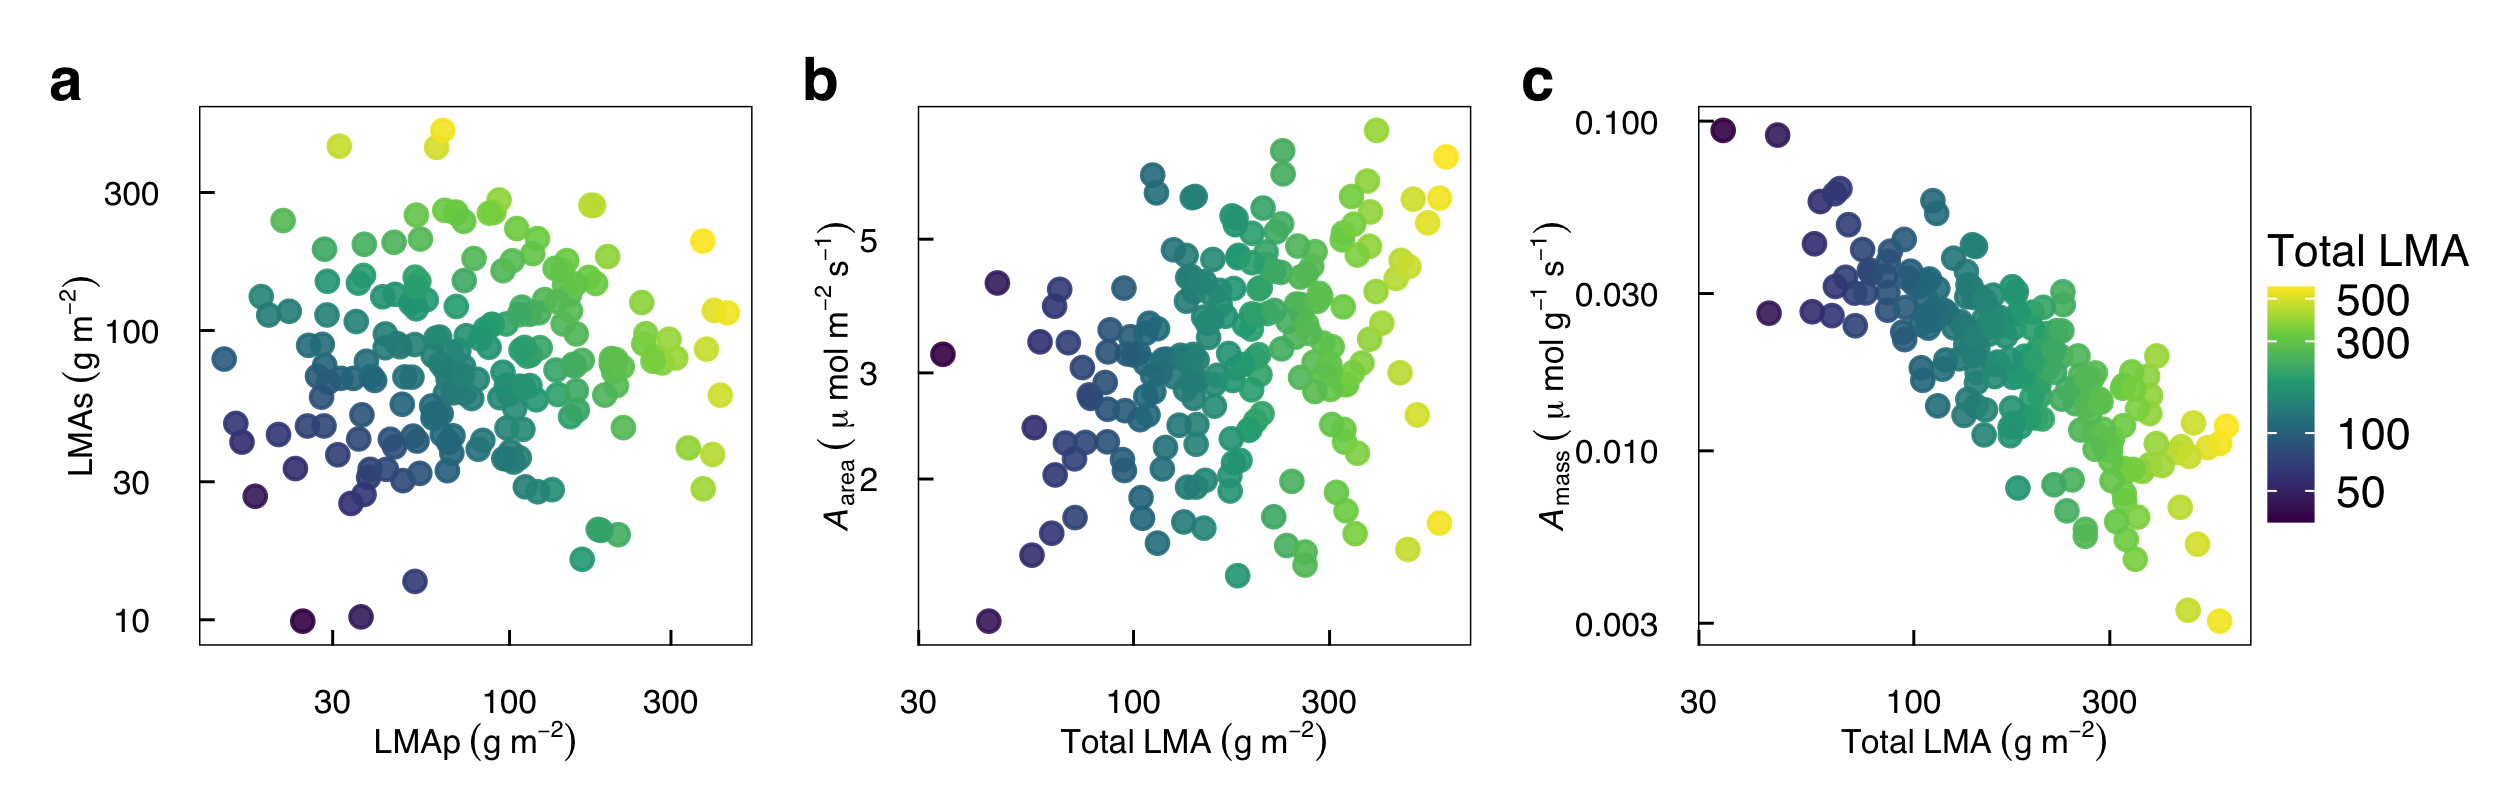
\includegraphics{../figs/fig_hypo.png}
%DIFDELCMD < \caption{Example of a two-dimensional functional space that can result in either a two- or one-dimensional trait space, depending on how metabolic traits are normalized. (A) Hypothetical indpendent variation in two leaf mass per area (LMA) components: metabolic leaf mass per area (LMAp, which largely determines per-area values of photosynthesis, respiration, and nutrient concentrations) and structural leaf mass per area (LMAs, which determines leaf toughness but has little effect on metabolic traits).
%DIFDELCMD < (B) Two-dimensional relationship between photosynthetic capacity (\emph{A}\textsubscript{max}) per-unit leaf area and total LMA (equal to LMAp + LMAs).
%DIFDELCMD < (C) One-dimensional relationship between \emph{A}\textsubscript{max} per-unit leaf mass and total LMA. Variation in LMAp and LMAs \emph{A}\textsubscript{max} values in panels B and C are derived from our analysis of the GLOPNET database. \(A_{\mathrm{area} \, i}=1.9\mathrm{LMAp}_i^{0.36}\mathrm{LMAs}^{-0.25}\epsilon_i\), where \(\epsilon_i\) is log-normally distributed with log-mean with 0, log-scale parameter with 0.3 (see Methods and Results).''\}}\label{fig:Hplt}
%DIFDELCMD < }
%DIFDELCMD < %%%
\DIFdelendFL \DIFaddbeginFL \hypertarget{fig:Hplt}{%
\centering
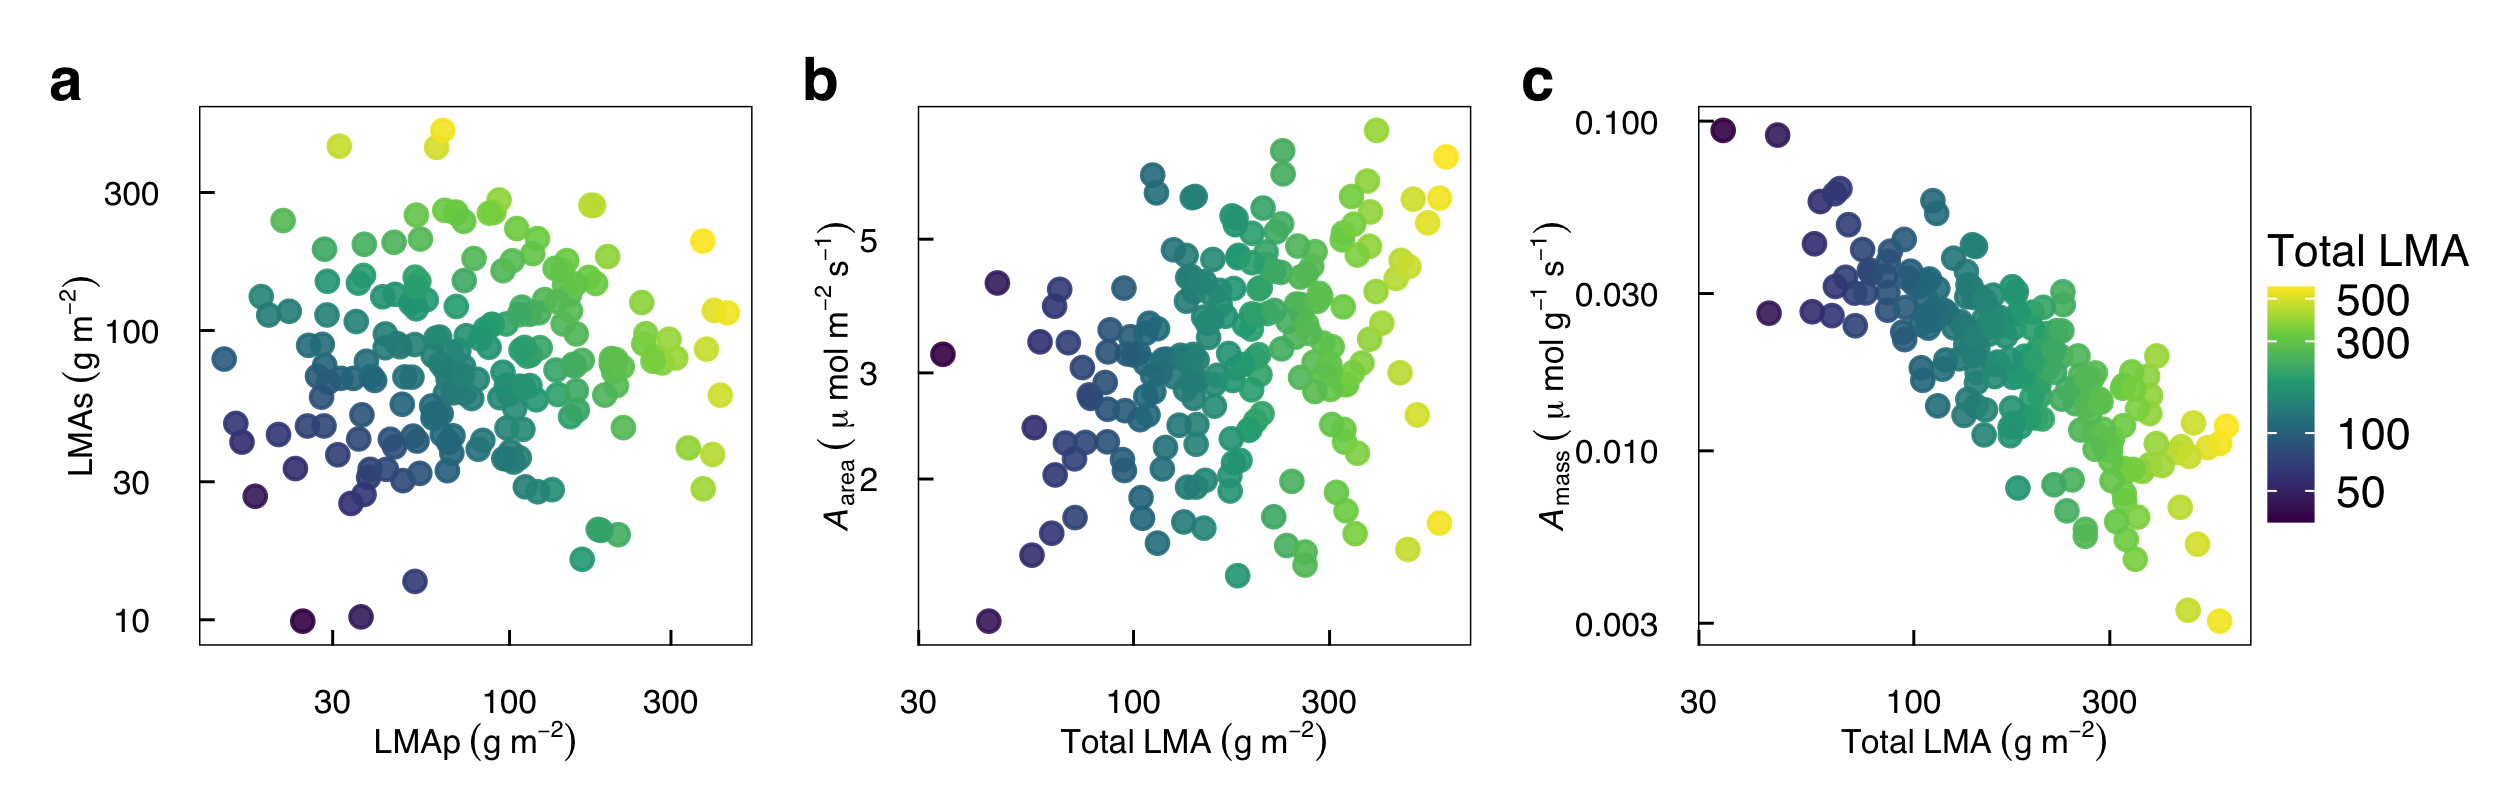
\includegraphics{../figs/fig_hypo.png}
\caption{Example of a two-dimensional functional space that can result in either a two- or one-dimensional trait space, depending on how metabolic traits are normalized. (A) Hypothetical independent variation in two leaf mass per area (LMA) components: metabolic leaf mass per area (LMAp, which largely determines per-area values of photosynthesis, respiration, and nutrient concentrations) and structural leaf mass per area (LMAs, which determines leaf toughness but has little effect on metabolic traits).
(B) Two-dimensional relationship between photosynthetic capacity (\emph{A}\textsubscript{max}) per-unit leaf area and total LMA (equal to LMAp + LMAs).
(C) One-dimensional relationship between \emph{A}\textsubscript{max} per-unit leaf mass and total LMA.
LMAp and LMAs are simulated from a hypothetical scenario of lognormal distributions with medians of 80 and standard deviations of exp(0.8) and exp(0.7), and zero covariance.
Variation in \emph{A}\textsubscript{max} values are derived from our analysis of the GLOPNET database. \(A_{\mathrm{area} \, i}=1.81\mathrm{LMAp}_i^{0.28}\mathrm{LMAs}^{-0.13}\epsilon_i\), where \(\epsilon_i\) is log-normally distributed with log-mean with 0, log-scale parameter with 0.31 (see Methods and Results).}\label{fig:Hplt}
}
\DIFaddendFL \end{figure}

\DIFdelbegin \DIFdel{\%s/}\DIFdelend \DIFaddbegin \begin{figure}
\hypertarget{fig:GLplt}{%
\centering
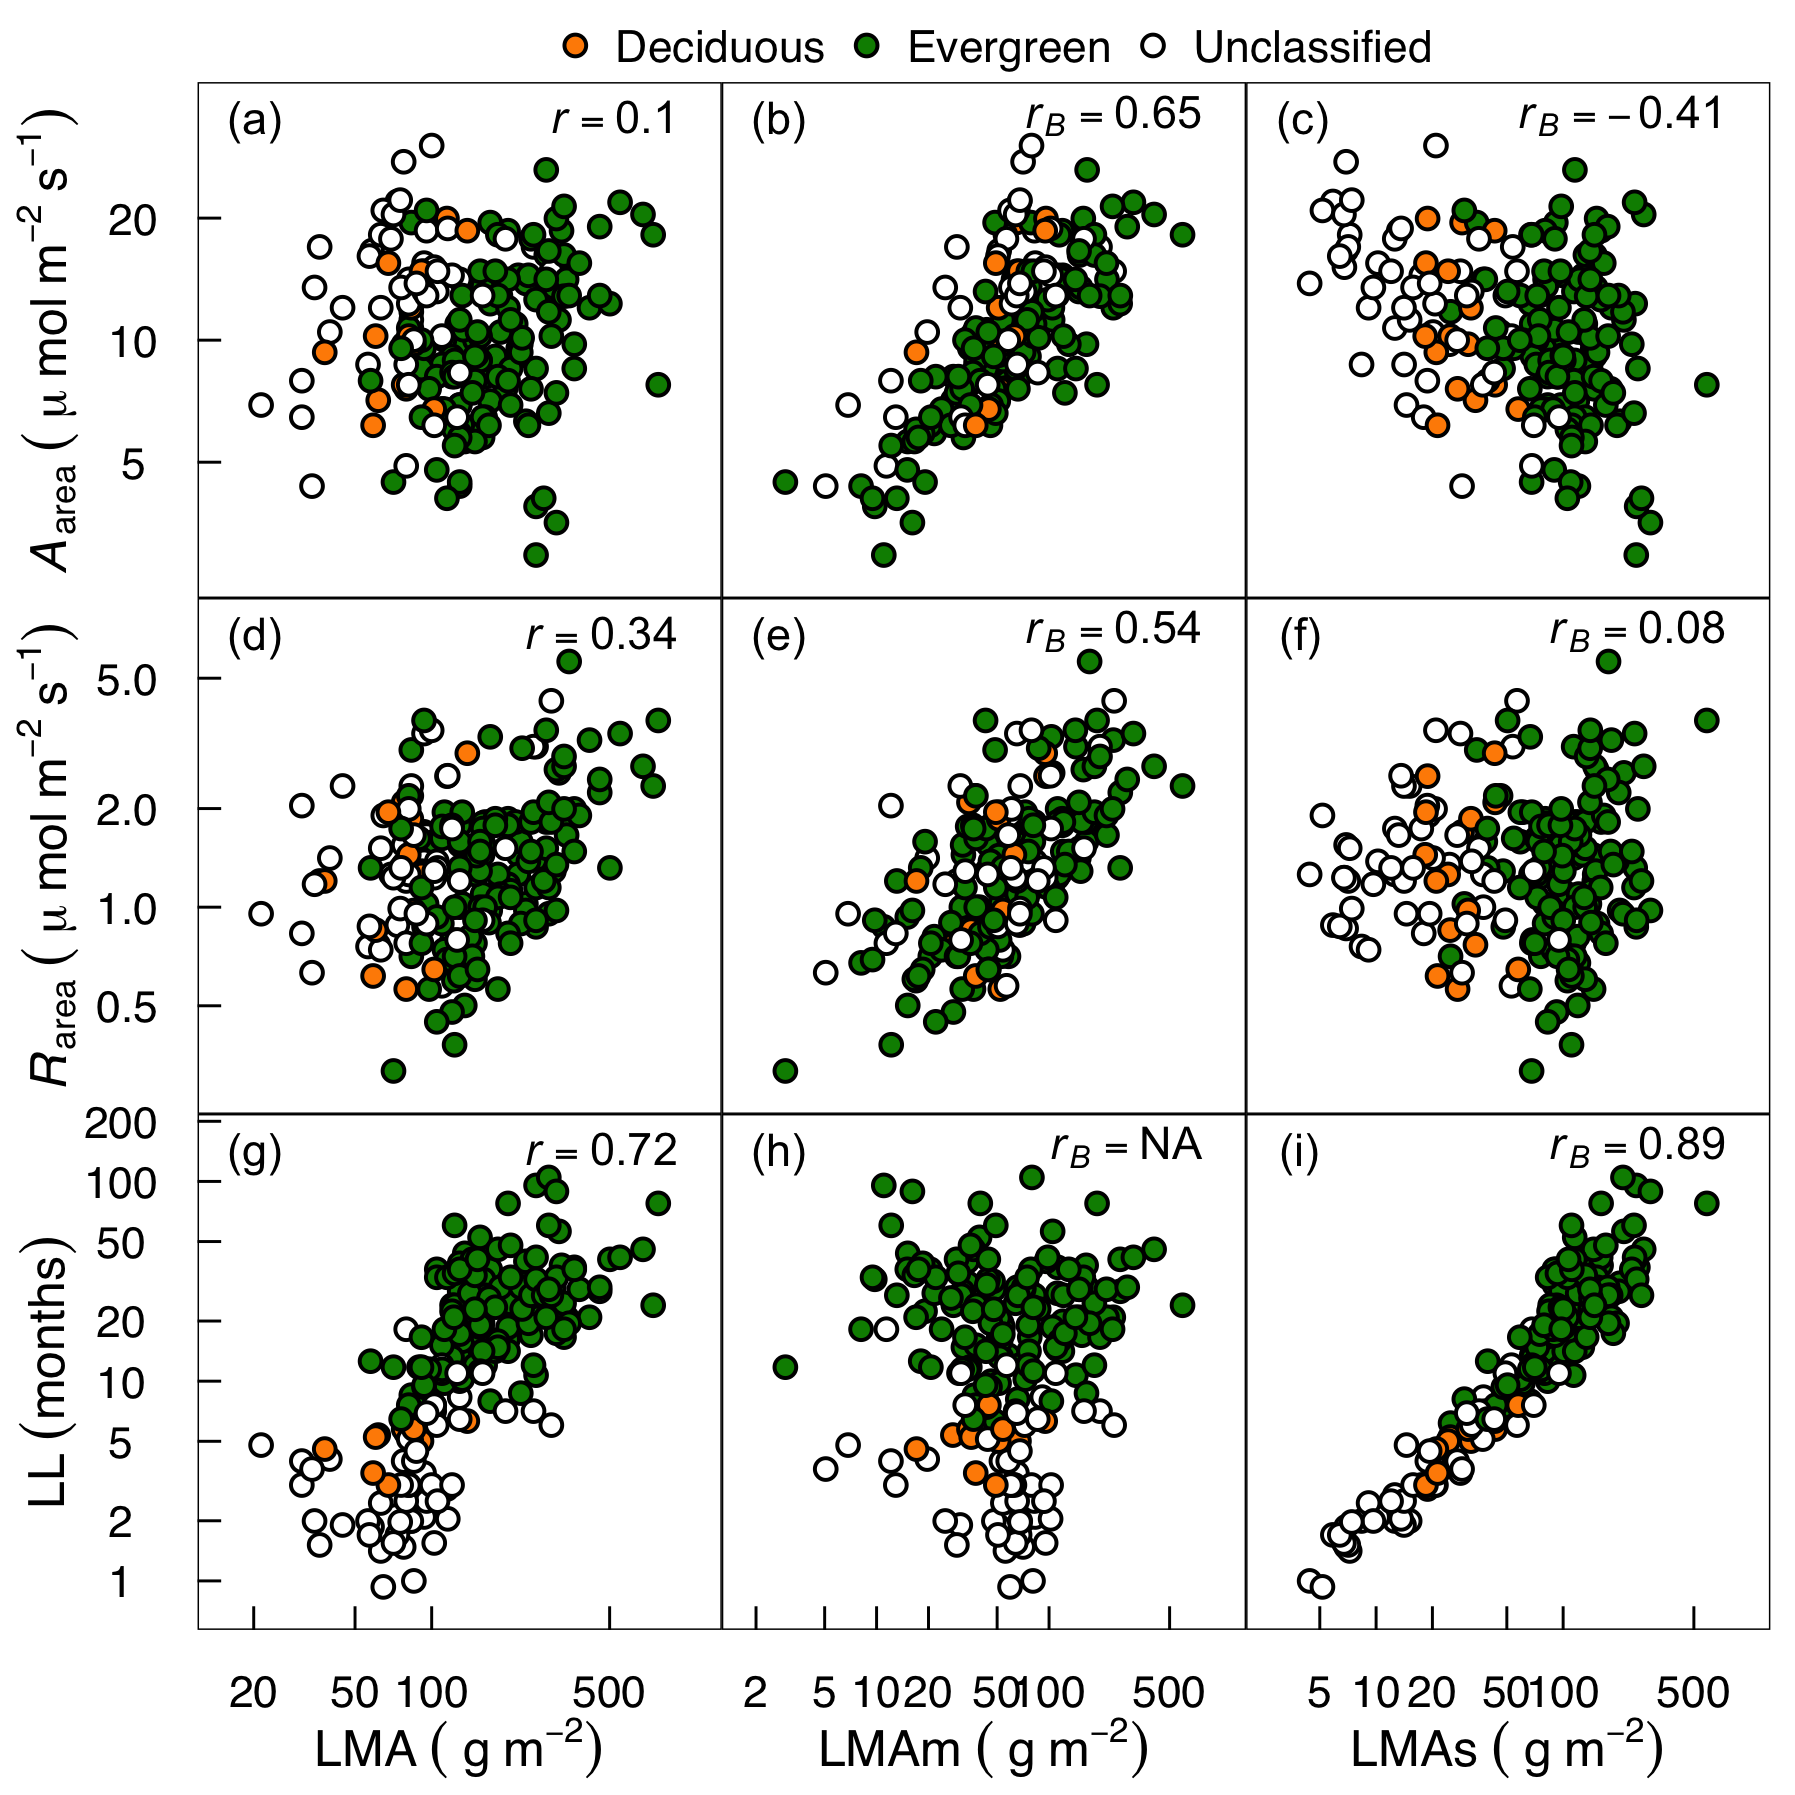
\includegraphics{../figs/GL_scatter.png}
\caption{Observed and estimated leaf-trait relationships in the global GLOPNET dataset.
Estimates are from the NAME Model (Eq. X).
Leaf life span (LL), net photosynthetic rate per unit leaf area (\emph{A}\textsubscript{area}), and dark respiration rate per unit leaf area (\emph{R}\textsubscript{area}) are plotted against observed LMA, posterior means of LMAp and LMAs.
Pearson correlation coefficients (\emph{r}) for LMA (left column) and posterior means of Pearson correlation coefficients (\(\bar{r}\)) or partial correlation coefficients (\(\bar{\rho}\)) of LMAp (middle column) and LMAs (right column) are shown.
Note that LL was modeled by LMAs alone.}\label{fig:GLplt}
}
\end{figure}

\DIFaddend \newpage
\DIFdelbegin \DIFdel{/\textbackslash newpage
}\DIFdelend 

\begin{figure}
\DIFdelbeginFL %DIFDELCMD < \hypertarget{fig:GLplt}{%
%DIFDELCMD < \centering
%DIFDELCMD < 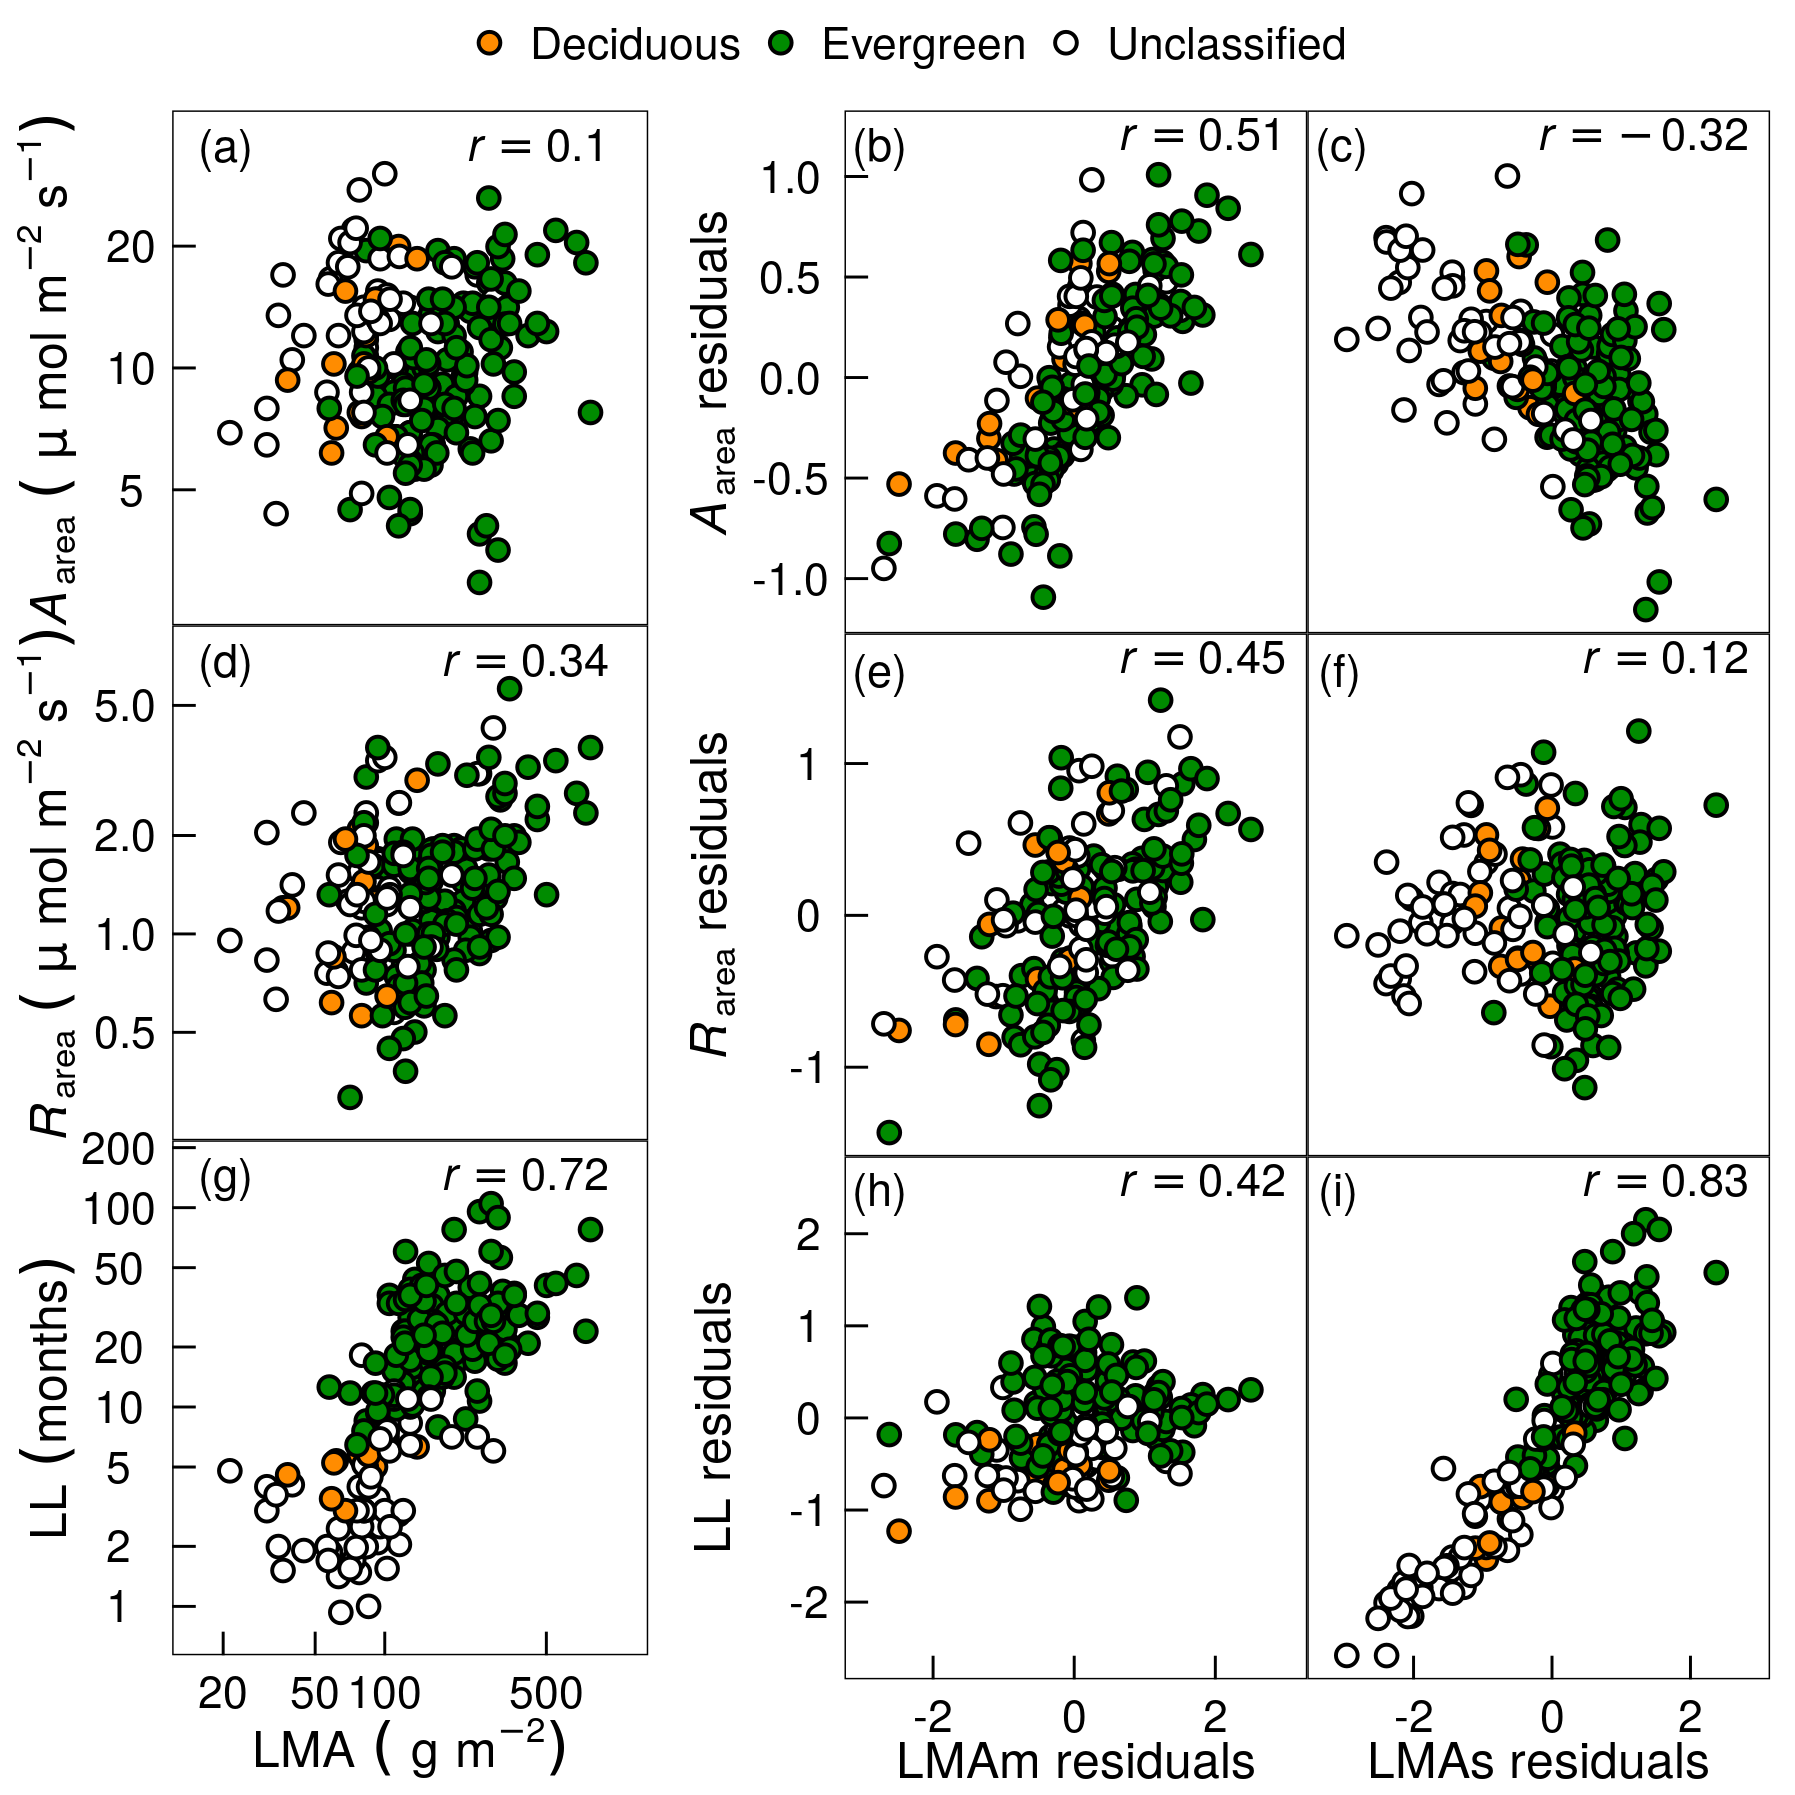
\includegraphics{../figs/GL_3.png}
%DIFDELCMD < \caption{Observed and estimated leaf-trait relationships in the global GLOPNET dataset.
%DIFDELCMD < (A) Leaf life span (LL), net photosynthetic rate per unit leaf area (\emph{A}\textsubscript{area}), and dark respiration rate per unit leaf area (\emph{R}\textsubscript{area}) are plotted against observed LMA.
%DIFDELCMD < (B) Residuals of LL, \emph{A}\textsubscript{area}, and \emph{R}\textsubscript{area} regressed on posteior estimates of photosynthetic and structural LMA components (LMAp and LMAs, respectively) are plotted against LMAp and LMAs (only means are shown).
%DIFDELCMD < Pearson correlation coefficients are for LMA (left column) and posterior distributions of LMAp (middle column) and LMAs (right column).}\label{fig:GLplt}
%DIFDELCMD < }
%DIFDELCMD < %%%
\DIFdelendFL \DIFaddbeginFL \hypertarget{fig:PAplt}{%
\centering
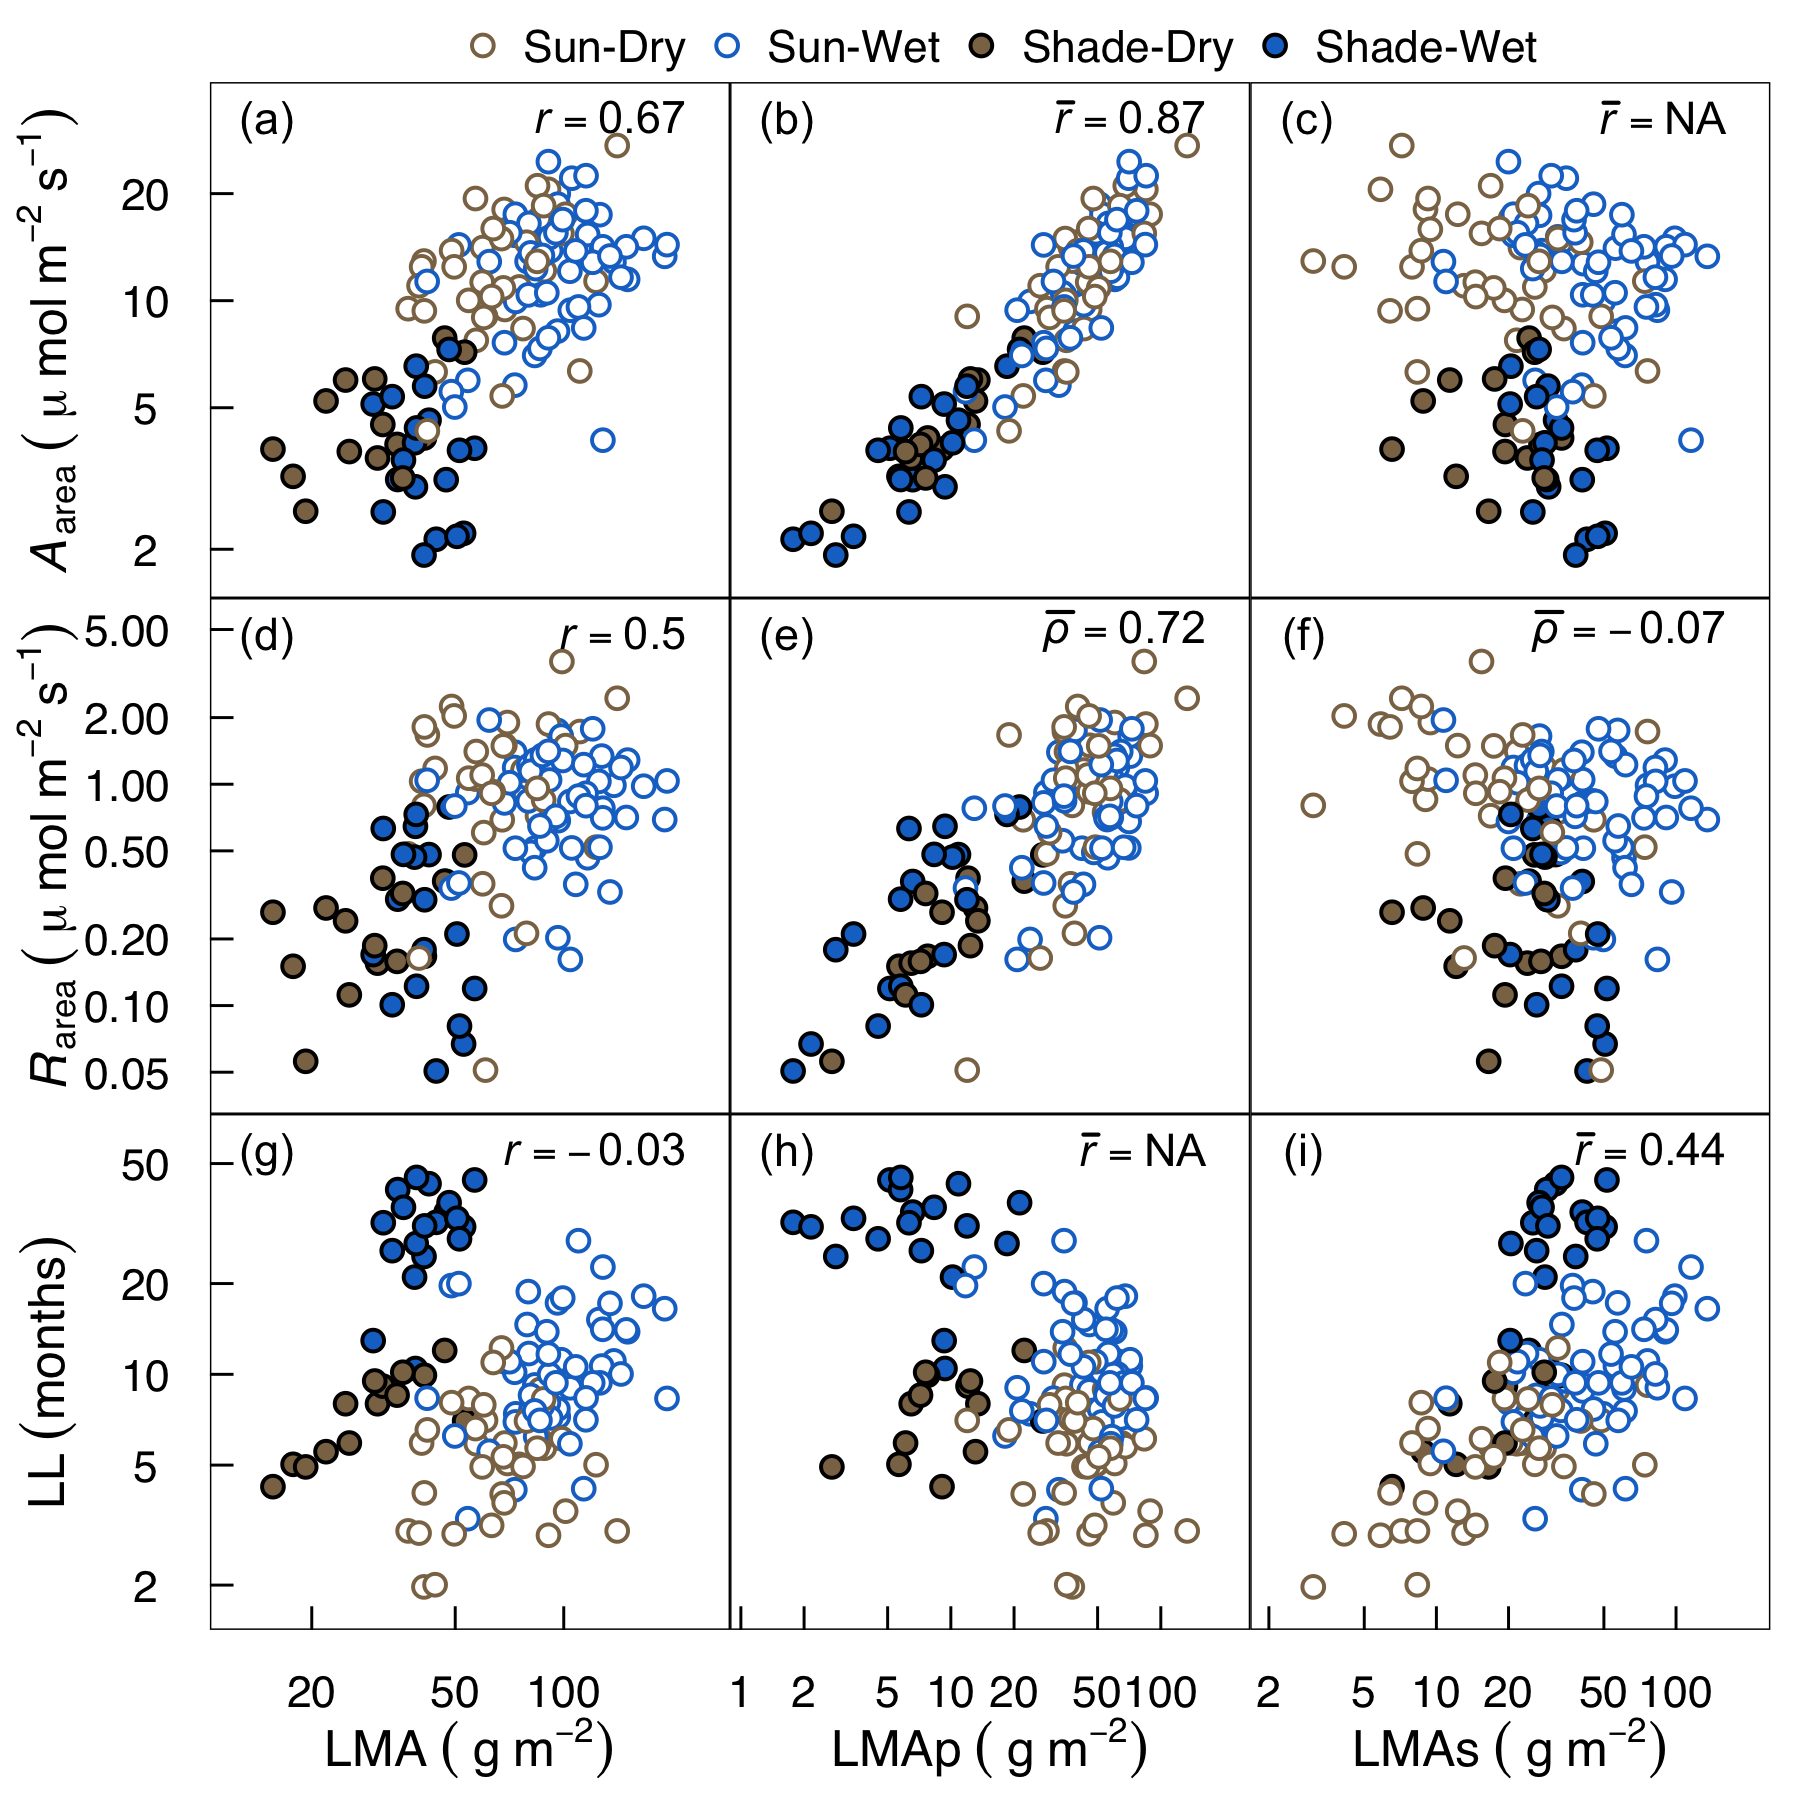
\includegraphics{../figs/PA_scatter.png}
\caption{Observed and estimated leaf-trait relationships in the Panama dataset.
Estimates are from the XXX Model (Eq. 6b).
Details as in Fig.~\ref{fig:GLplt}.
Results for other LL models are summarized in Table SX.
Note that \emph{A}\textsubscript{area} and LL were modeled by LMAp and LMAs alone, respectively.}\label{fig:PAplt}
}
\DIFaddendFL \end{figure}

\newpage

\begin{figure}
\DIFdelbeginFL %DIFDELCMD < \hypertarget{fig:PAplt}{%
%DIFDELCMD < \centering
%DIFDELCMD < 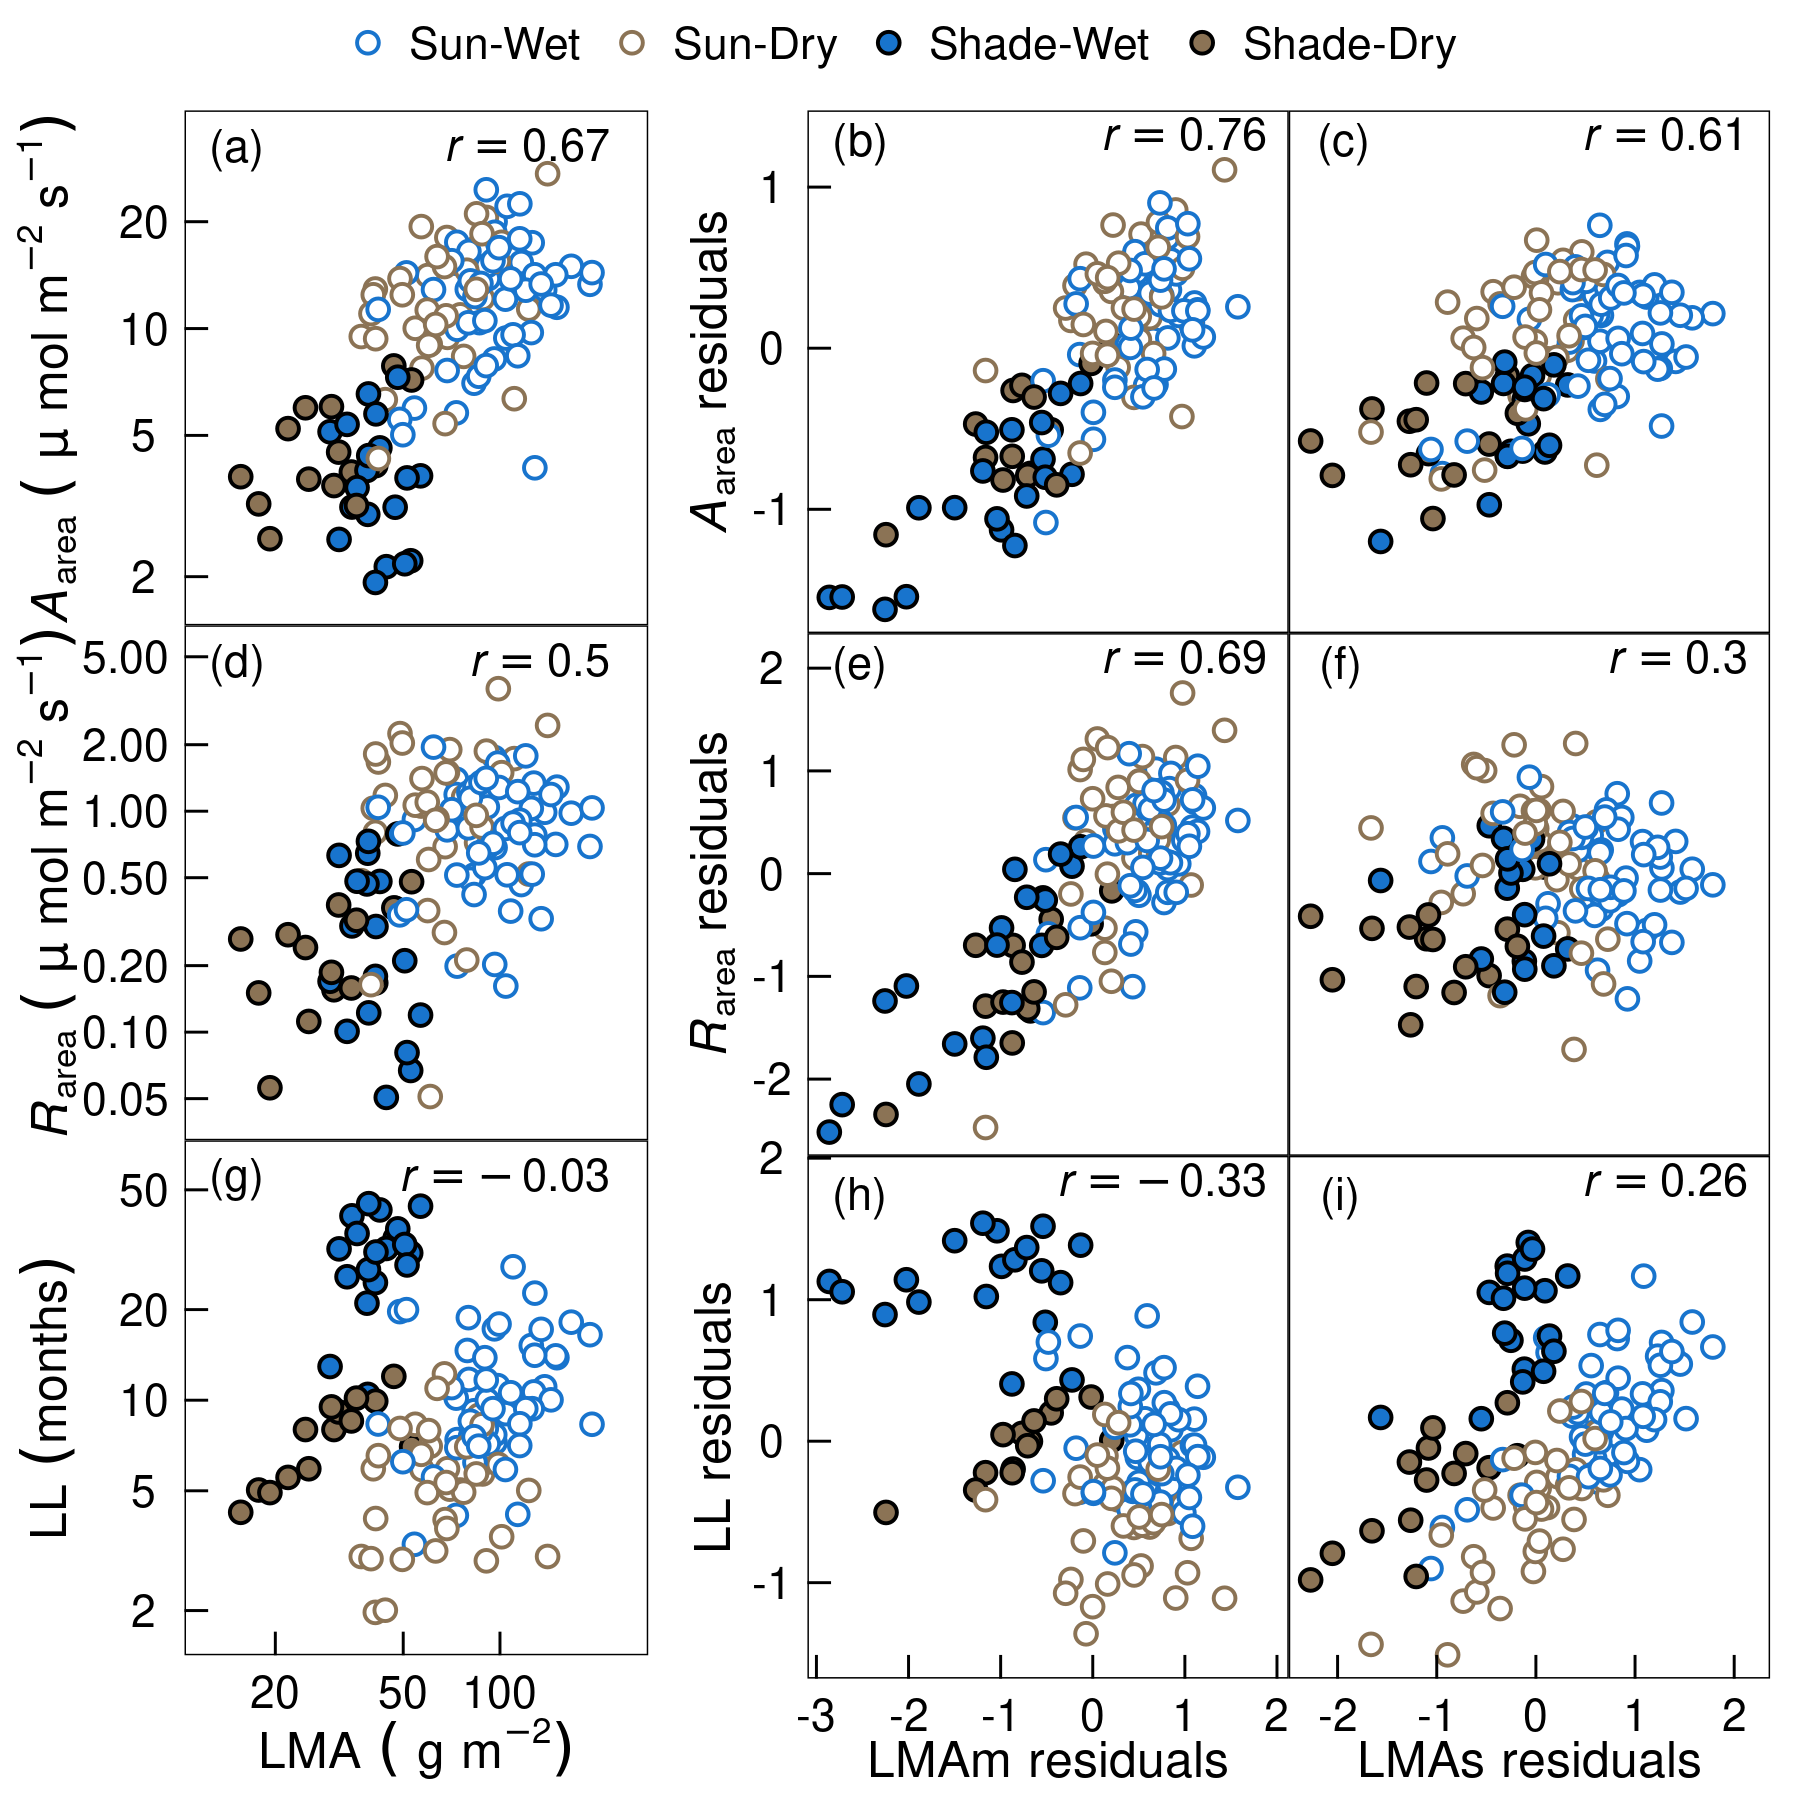
\includegraphics{../figs/PA_3.png}
%DIFDELCMD < \caption{Observed and estimated leaf-trait relationships in the Panama dataset. Estimates are from the Optimal LL Model (Eq. 8). Details as in Fig. 2. Results for other LL models are summarized in Table SX.}\label{fig:PAplt}
%DIFDELCMD < }
%DIFDELCMD < %%%
\DIFdelendFL \DIFaddbeginFL \hypertarget{fig:LLplt}{%
\centering
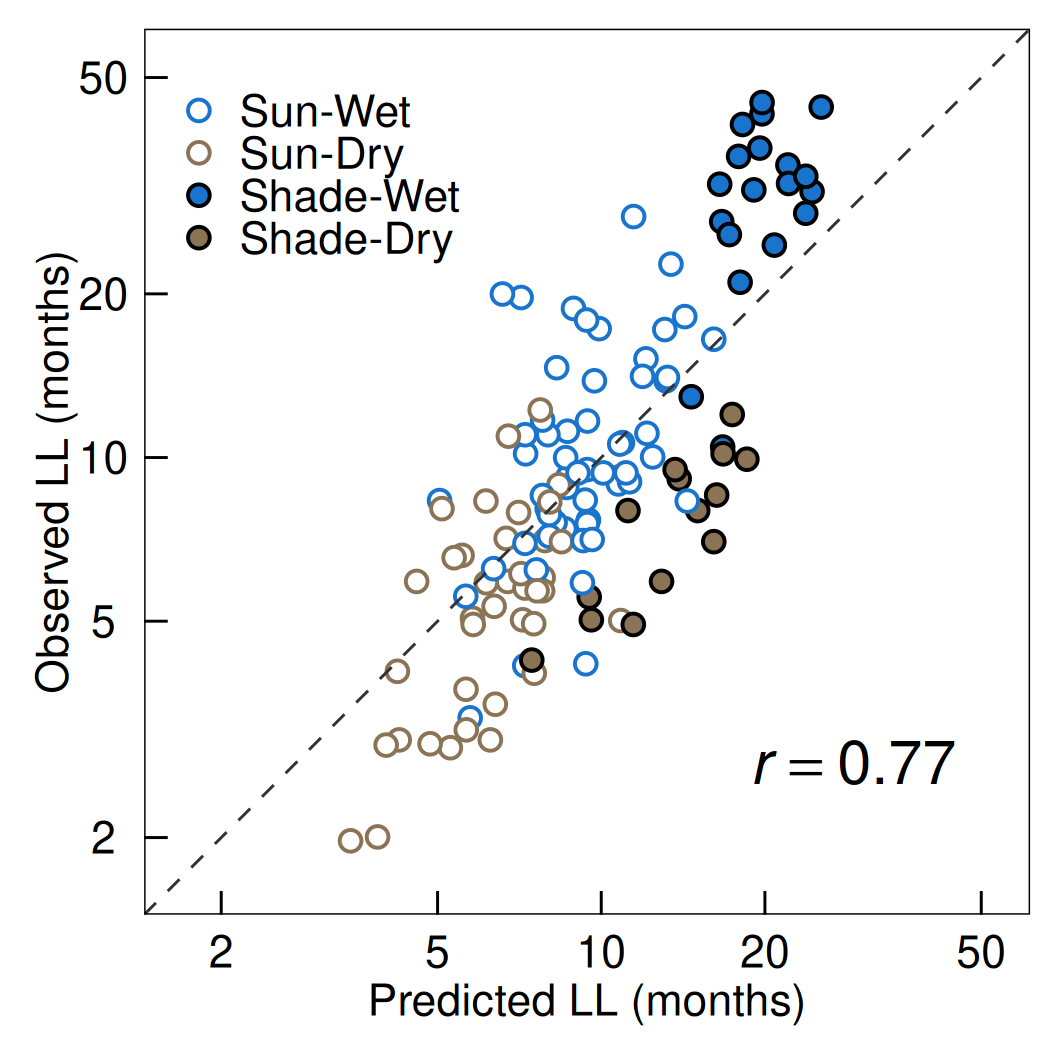
\includegraphics{../figs/LL_plot.png}
\caption{Observed vs.~predicted leaf lifespan (LL) in the LL with light Model (Eq. 6b).
Predicted LL values are posterior means.
The dashed line indicates the 1:1 relationship.
The \emph{R}\textsuperscript{2} value is the posterior mean of Bayesian \emph{R}\textsuperscript{2} (\protect\hyperlink{ref-Gelman2019}{Gelman et al. 2019}).}\label{fig:LLplt}
}
\DIFaddendFL \end{figure}

\newpage

\begin{figure}
\DIFdelbeginFL %DIFDELCMD < \hypertarget{fig:LLplt}{%
%DIFDELCMD < \centering
%DIFDELCMD < 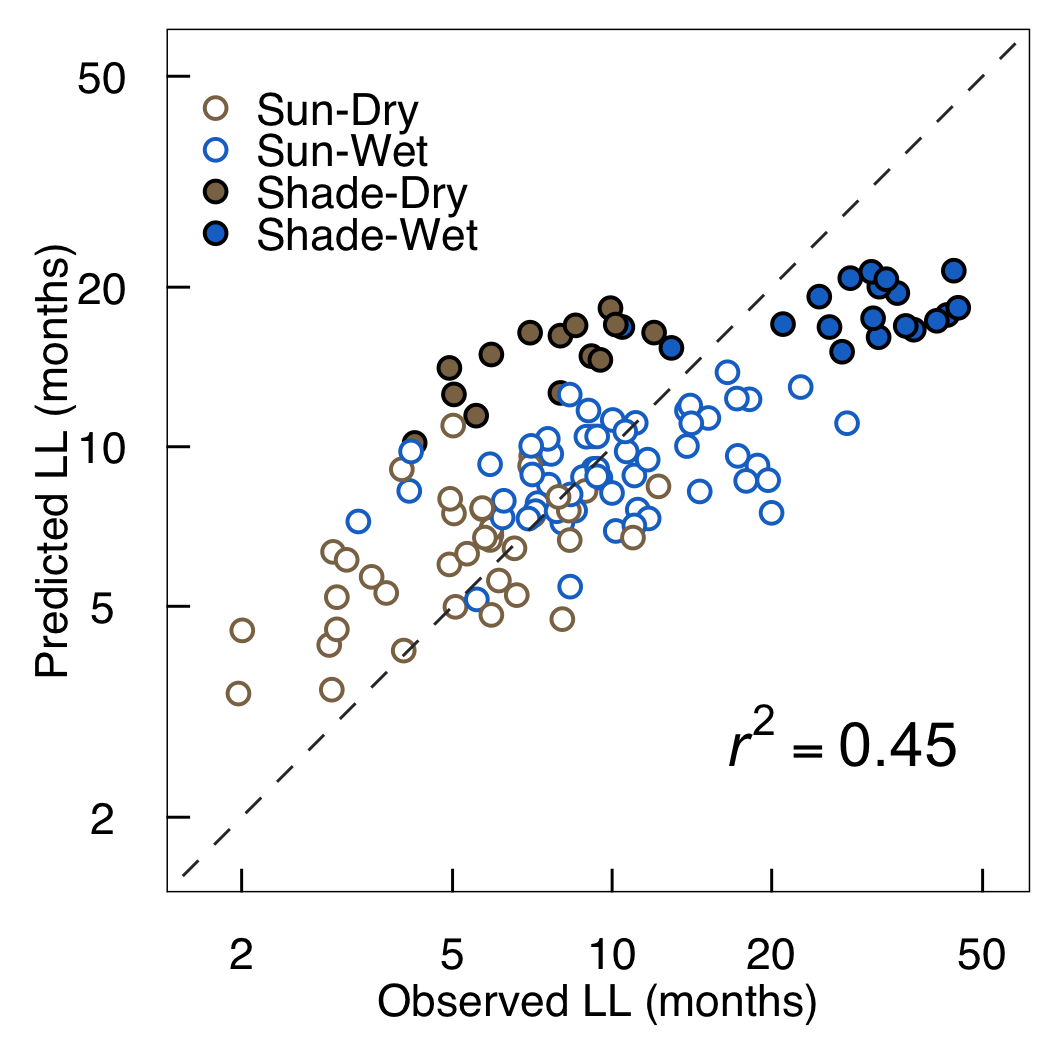
\includegraphics{../figs/LL_plot2.png}
%DIFDELCMD < \caption{Observed vs.~predicted leaf lifespan (LL) in the Optimal LL Model (Eq. 8).
%DIFDELCMD < Predicted LL values are posterior medians.
%DIFDELCMD < The dashed line indicates the 1:1 relationship.
%DIFDELCMD < The \emph{r}\textsuperscript{2} value is the posterior median of Bayesian \emph{r}\textsuperscript{2} (Gelman et al.~2019).}\label{fig:LLplt}
%DIFDELCMD < }
%DIFDELCMD < %%%
\DIFdelendFL \DIFaddbeginFL \hypertarget{fig:massplt}{%
\centering
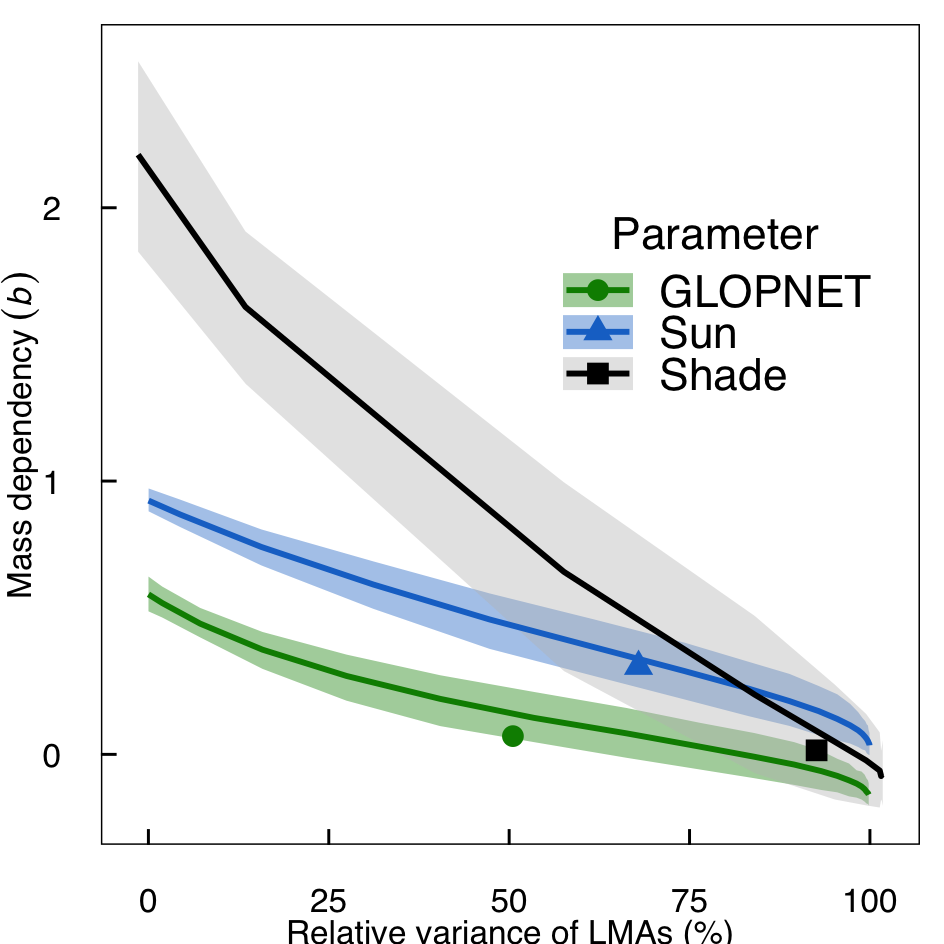
\includegraphics{../figs/mass_prop_simple.png}
\caption{The relationships between mass dependency (\emph{b} in Eq. 8) and relative variance in LMAs to LMA for the global GLOPNET dataset, sun leaves in Panama, and shade leaves in Panama.
Solid lines indicate simulated means and shaded regions indicate 95\% CI.
Each symbol indicates the estimated values from the empirical data.
The photosynthetic rate (\emph{A}\textsubscript{max}) is primarily mass-dependent (\emph{b} \textgreater{} 0.5), primarily area-dependent (0.5 \textgreater{} \emph{b} \textgreater{} 0) and purely area-dependent (\emph{b} = 0) (\protect\hyperlink{ref-Osnas2018}{Osnas et al. 2018}).
Note that when \emph{b} \textgreater{} 1, \emph{A}\textsubscript{area} dramatically increases with LMA, which is not realistic.}\label{fig:massplt}
}
\DIFaddendFL \end{figure}

\newpage

\begin{figure}
\DIFdelbeginFL %DIFDELCMD < \hypertarget{fig:massplt}{%
%DIFDELCMD < \centering
%DIFDELCMD < 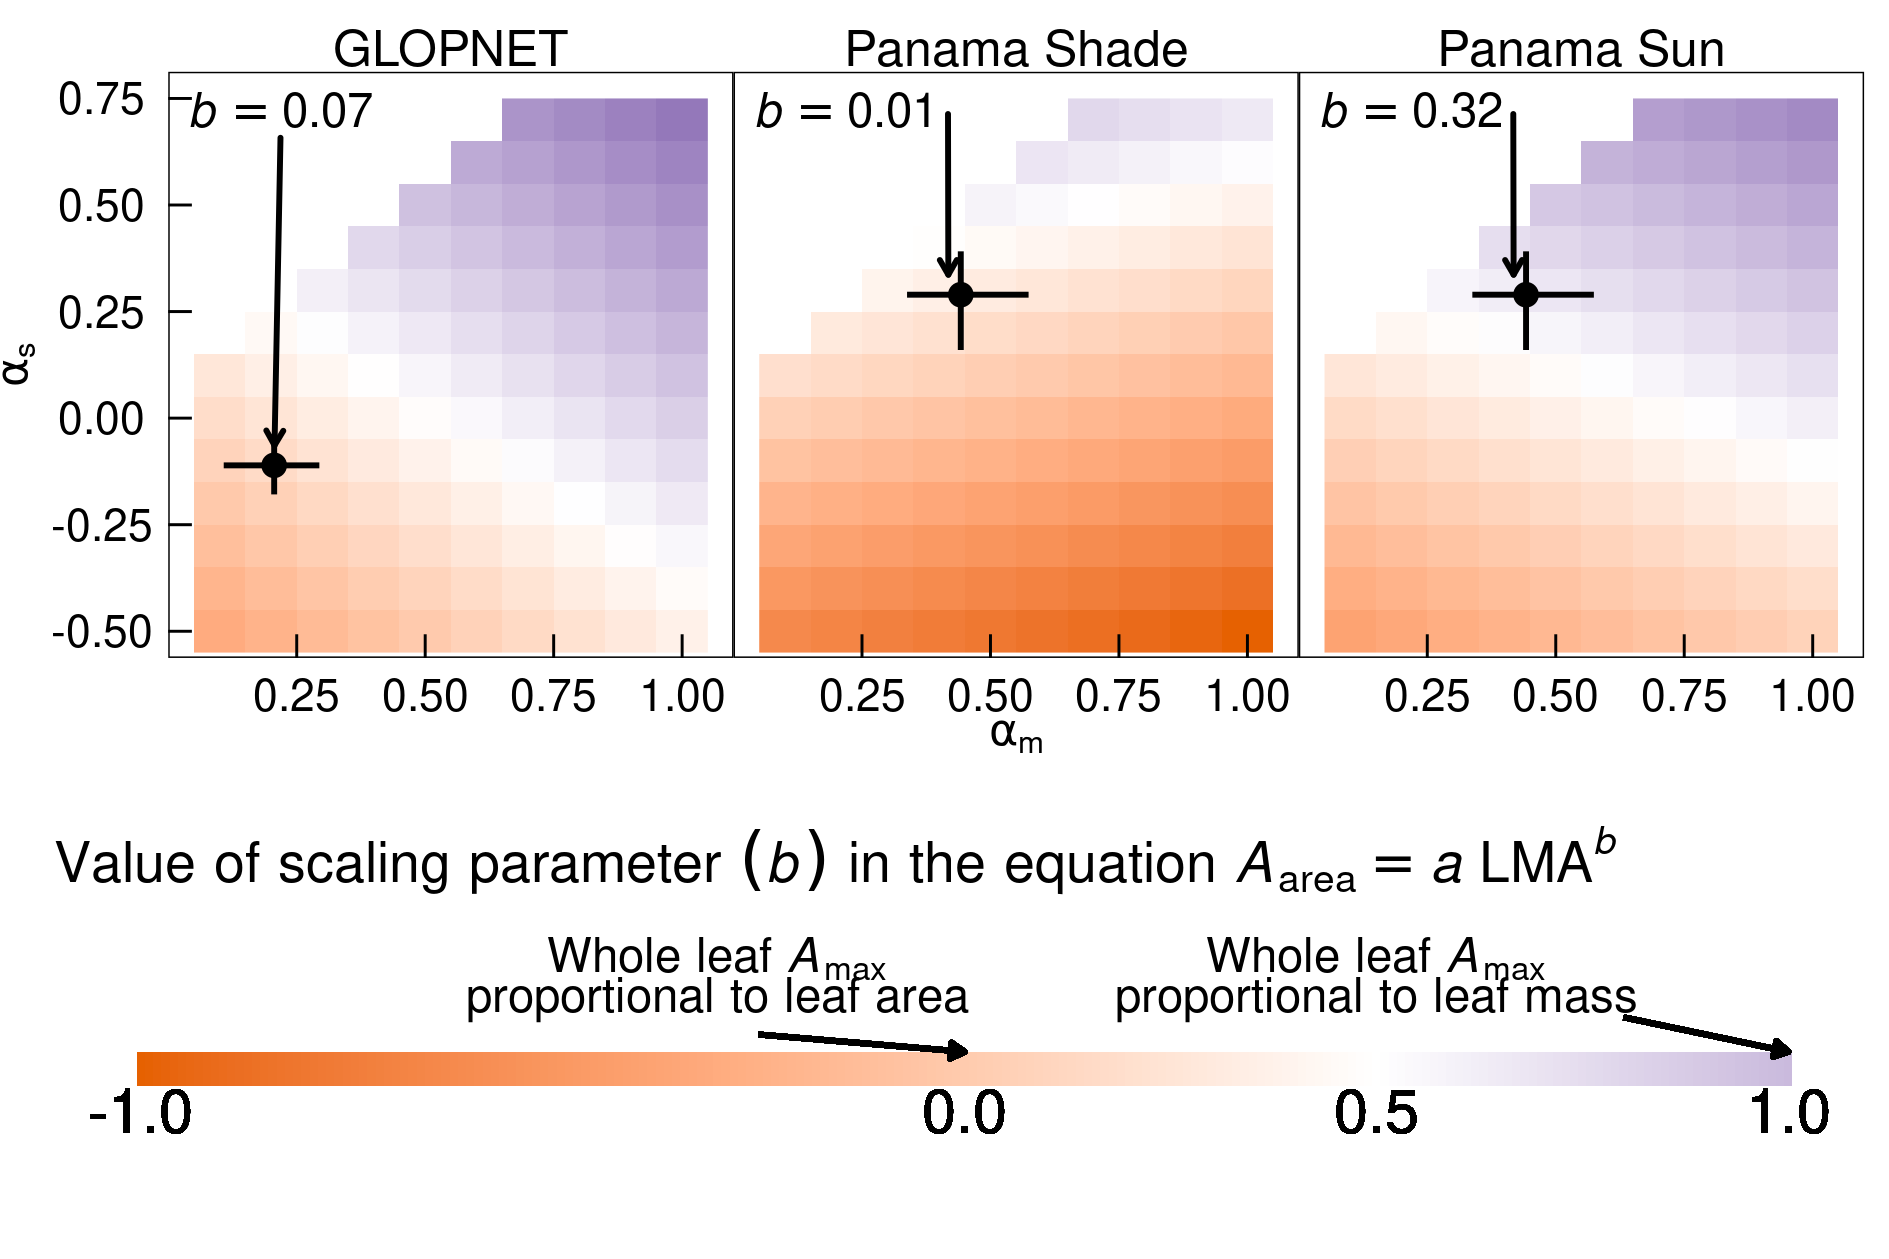
\includegraphics{../figs/mass_prop4.png}
%DIFDELCMD < \caption{The relationships among mass proportionality (\emph{b\textsubscript{i}} in Eq. 8), variance in LMAp and LMAs, and scaling slopes between LMAp and \emph{A}\textsubscript{area} (\(\alpha_p\)) and LMAs and \emph{A}\textsubscript{area} (\(\alpha_s\)) for the global GLOPNET dataset, sun leaves in Panama, and shade leaves in Panama.
%DIFDELCMD < The photosynthetic rate (\emph{A}\textsubscript{max}) is primarily mass-dependent (\emph{b\textsubscript{i}} \textgreater{} 0.5, white to blue), primarily area-dependent (0.5 \textgreater{} \emph{b\textsubscript{i}} \textgreater{} 0, white to orange) and purely area-proportional (\emph{b\textsubscript{i}} = 0, white) (Osnas et al.~2018).
%DIFDELCMD < Note that when \emph{b\textsubscript{i}} is negative, \emph{A}\textsubscript{area} decreases with LMA, which is not realistic.}\label{fig:massplt}
%DIFDELCMD < }
%DIFDELCMD < %%%
\DIFdelendFL \DIFaddbeginFL \hypertarget{fig:vpart}{%
\centering
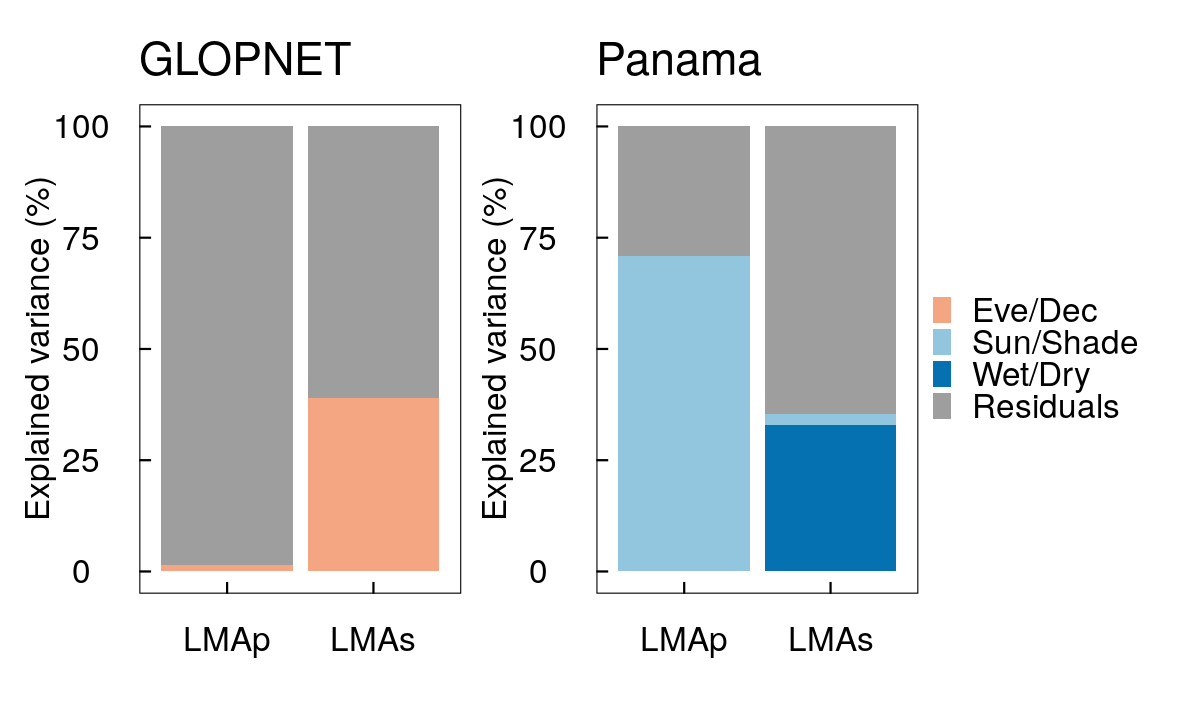
\includegraphics{../figs/vpart.png}
\caption{Variance partitioning on LMA components between and within leaf habits (evergreen vs.~deciuous) for the GLOPNET dataset, and between and within sites (wet vs.~dry) and light (sun vs.~shade) for the Panama dataset.}\label{fig:vpart}
}
\DIFaddendFL \end{figure}

\newpage

\begin{figure}
\hypertarget{fig:boxplt}{%
\centering
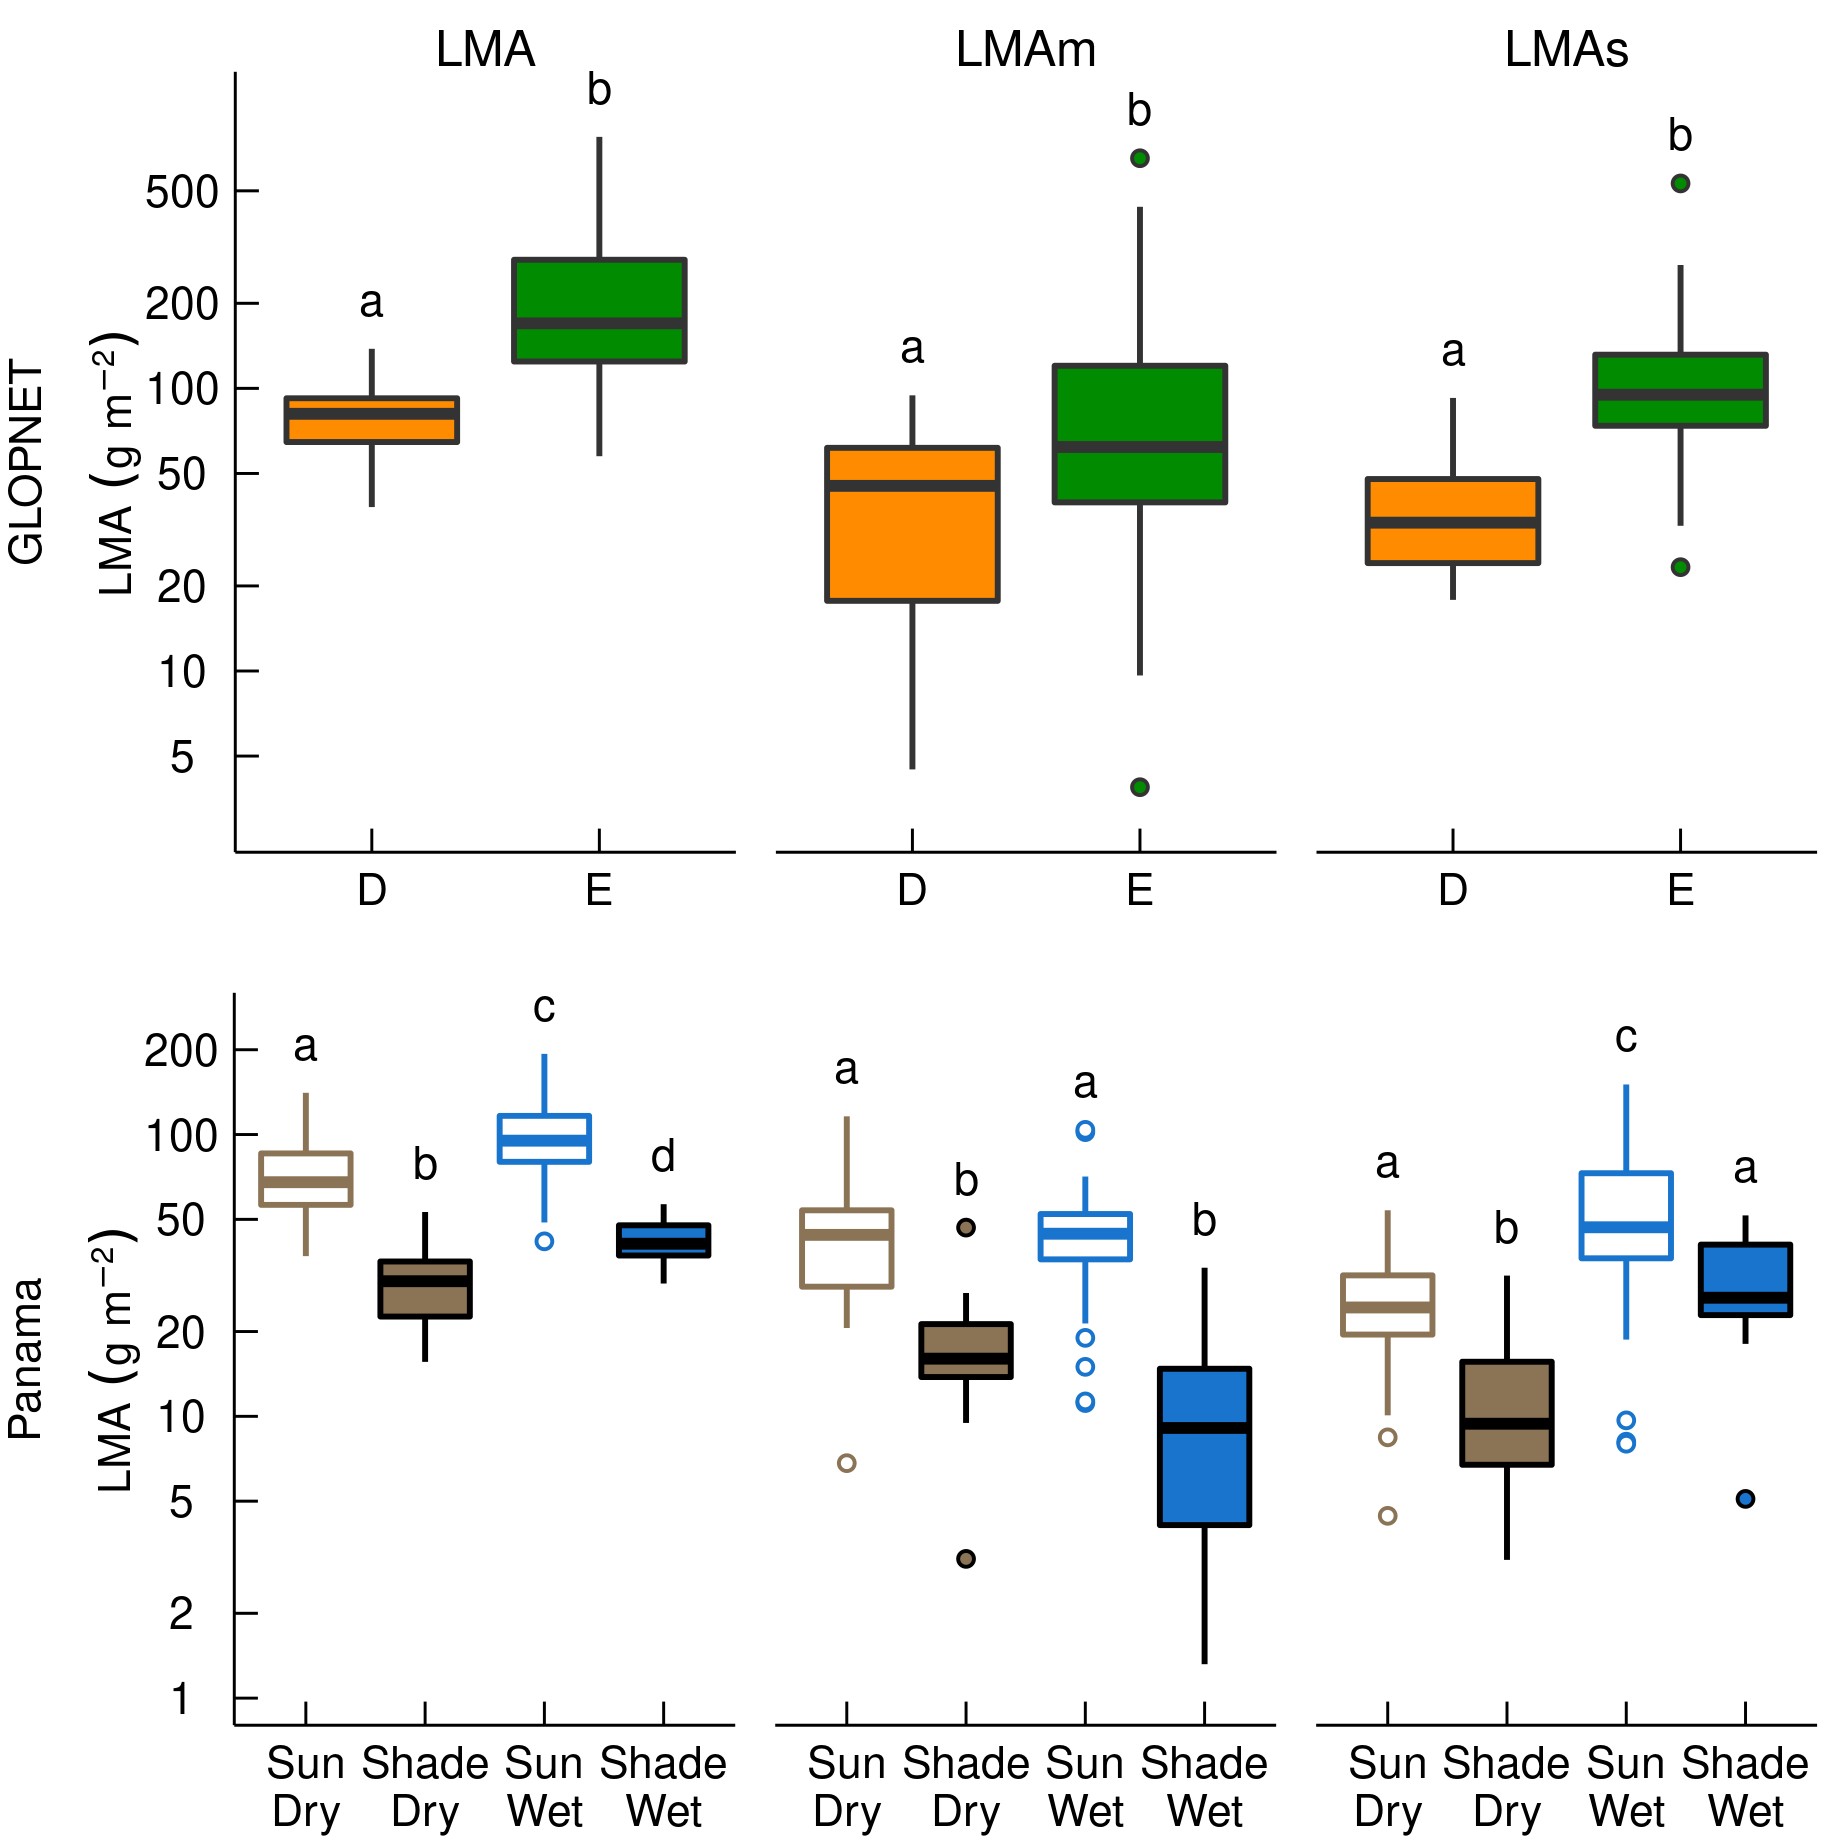
\includegraphics{../figs/box_main.png}
\caption{Boxplots comparing leaf mass per area (LMA) and posterior medians of photosynthetic and structural LMA components (LMAp and LMAs, respectively) across deciduous (D) and evergreen (E) leaves in the GLOPNET dataset (top), and across sites (wet and dry) and canopy strata (sun and shade) in the Panama dataset (bottom).
The center line in each box indicates the median, upper and lower box edges indicate the interquartile range, whiskers show 1.5 times the interquartile range, and points are outliers.
Groups sharing the same letters are not significantly different (P \textgreater{} 0.05; t-tests).
To isolate the effects of intraspecific variation (i.e., plastic responses to light), the Panama results shown here only include species for which both sun and shade leaves were available.
Qualitatively similar results were obtained when all Panama species were included (Fig. SX).
Note that the vertical axis is on a log\textsubscript{10} scale.}\label{fig:boxplt}
}
\end{figure}

\newpage

\begin{figure}
\DIFdelbeginFL %DIFDELCMD < \hypertarget{fig:PA-NPC}{%
%DIFDELCMD < \centering
%DIFDELCMD < 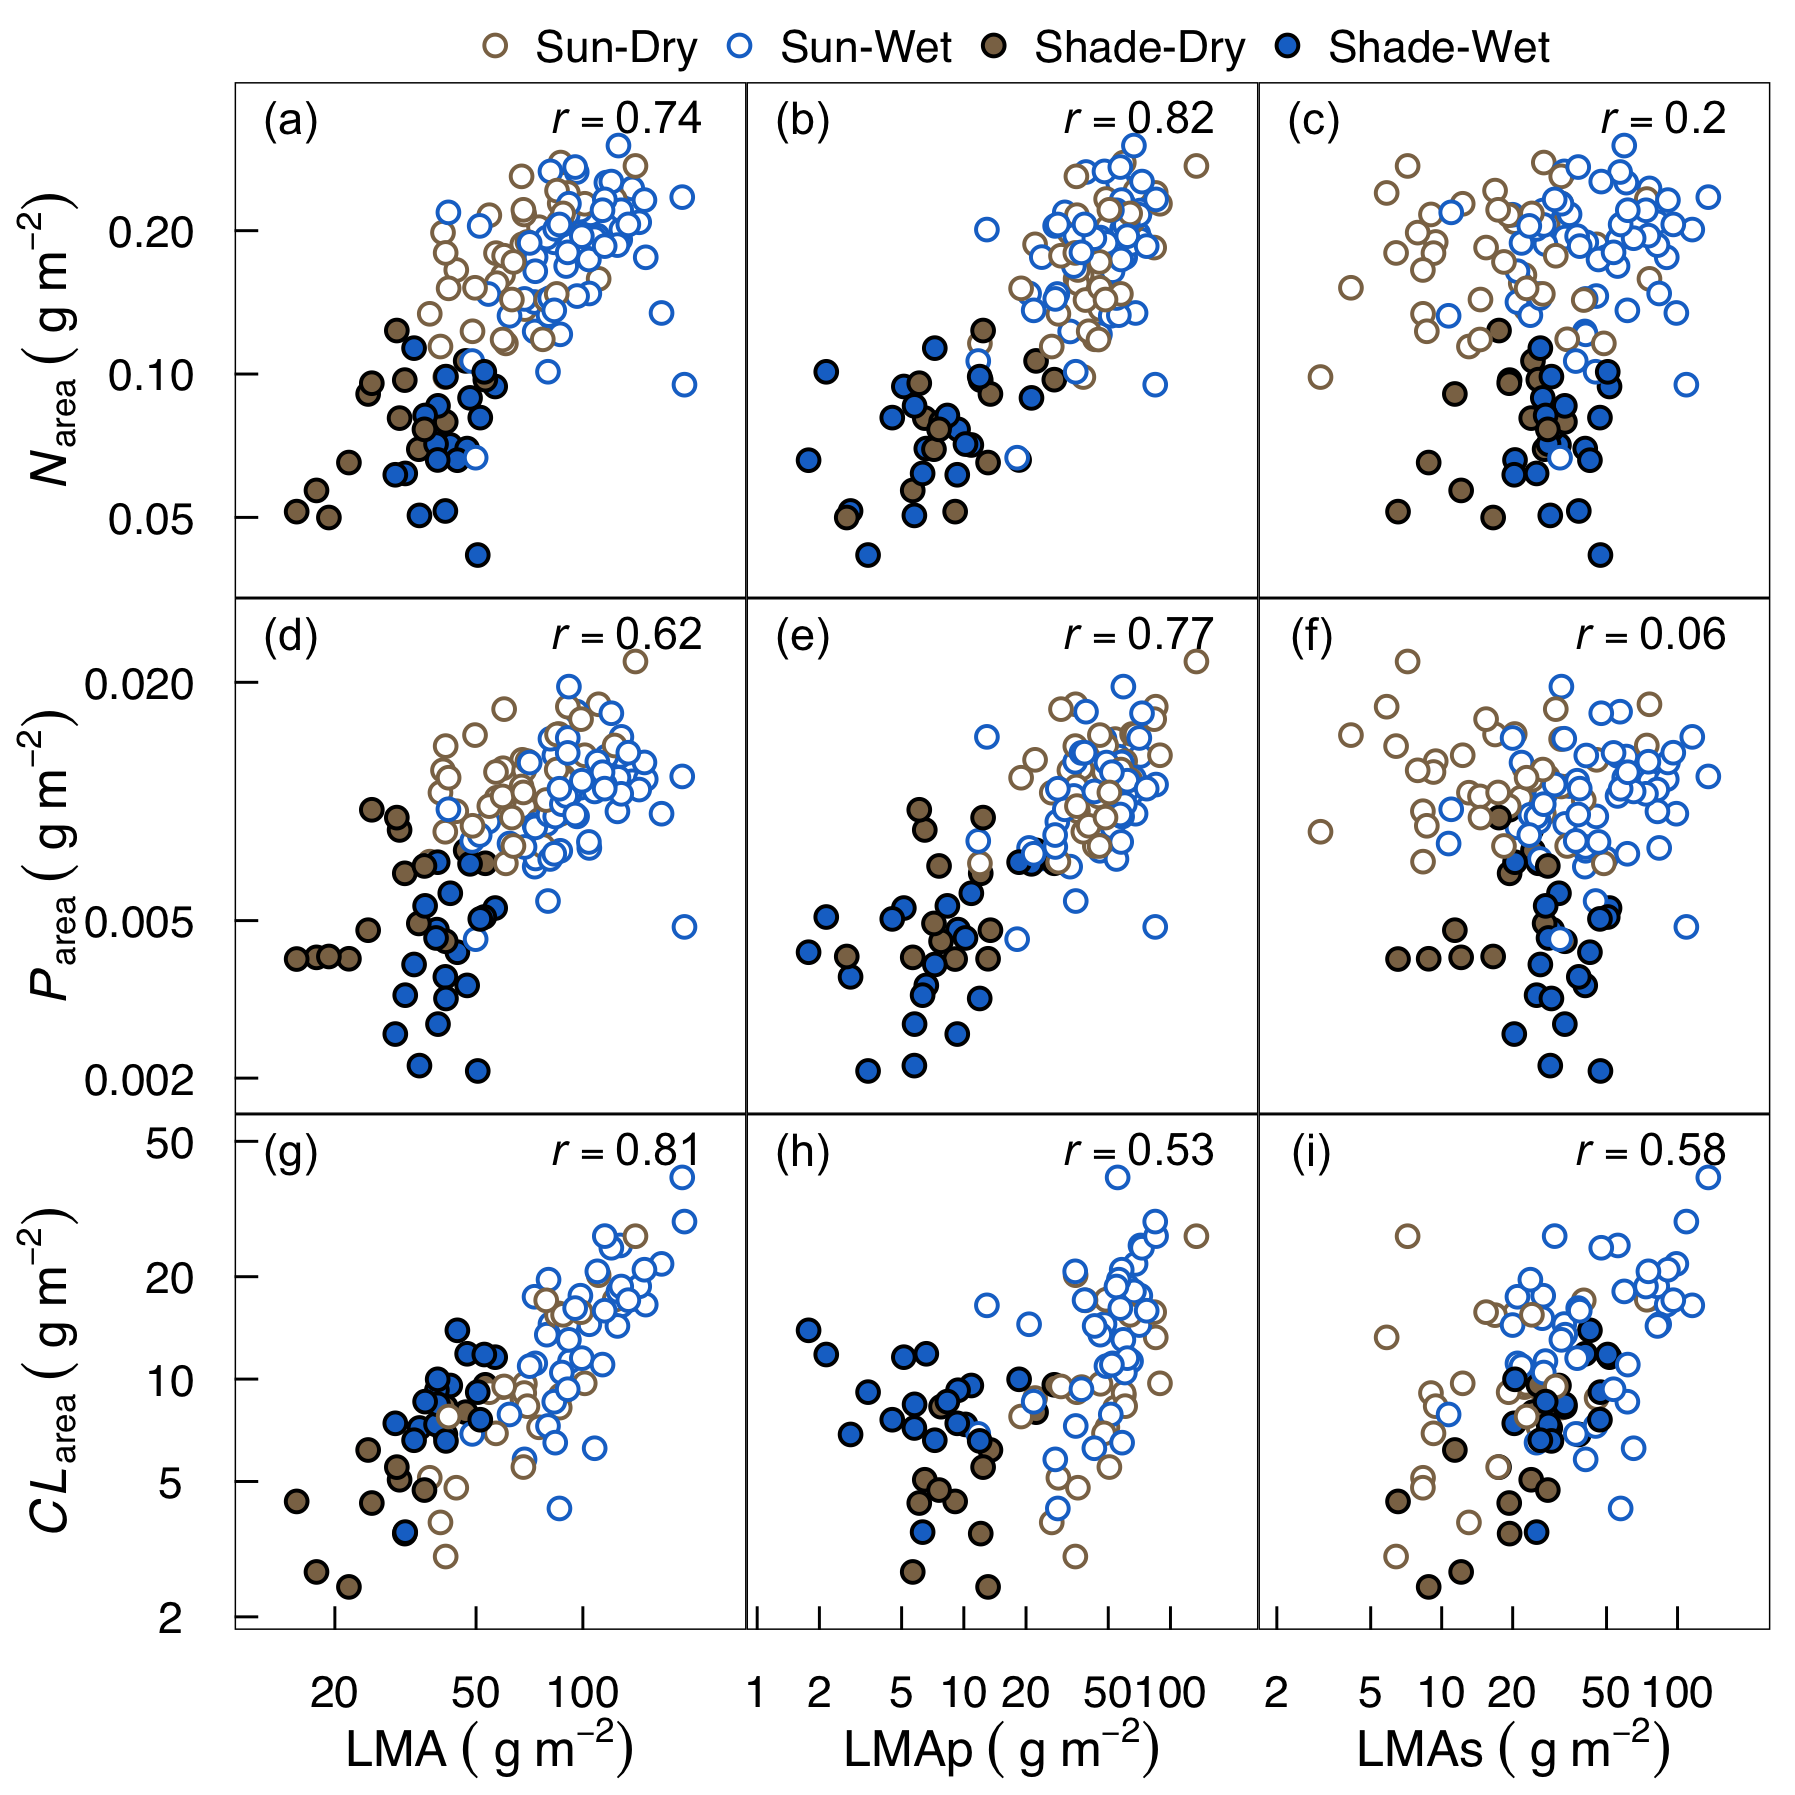
\includegraphics{../figs/PA_NPC.png}
%DIFDELCMD < \caption{Measured traits related to photosynthesis and metabolism traits (nitrogen and phosphorus per-unit leaf area; \emph{N}\textsubscript{area} and \emph{P}\textsubscript{area}) are strongly correlated with estimates (posterior medians) of the photosynthetic LMA component (LMAp), and a measured structural trait (cellulose per-unit leaf area; \emph{CL}\textsubscript{area}) is strongly correlated with estimates of the structural LMA component (LMAs) for the Panama dataset.
%DIFDELCMD < Note that sun and shade leaves align along a single relationship for \emph{CL}\textsubscript{area} vs.~LMAs, but not for \emph{CL}\textsubscript{area} vs.~LMA or LMAp. \emph{N}\textsubscript{area}, \emph{P}\textsubscript{area}, and \emph{CL}\textsubscript{area} data were not used to fit the models, and are presented here as independent support for the model results.
%DIFDELCMD < Analogous results were obtained for \emph{N}\textsubscript{area} and \emph{P}\textsubscript{area} vs.~LMAp for GLOPNET (Fig. S3).
%DIFDELCMD < Others details as in Fig. GL.
%DIFDELCMD < Results for other LL models are reported in Table SX.''\}}\label{fig:PA-NPC}
%DIFDELCMD < }
%DIFDELCMD < %%%
\DIFdelendFL \DIFaddbeginFL \hypertarget{fig:PA-NPC}{%
\centering
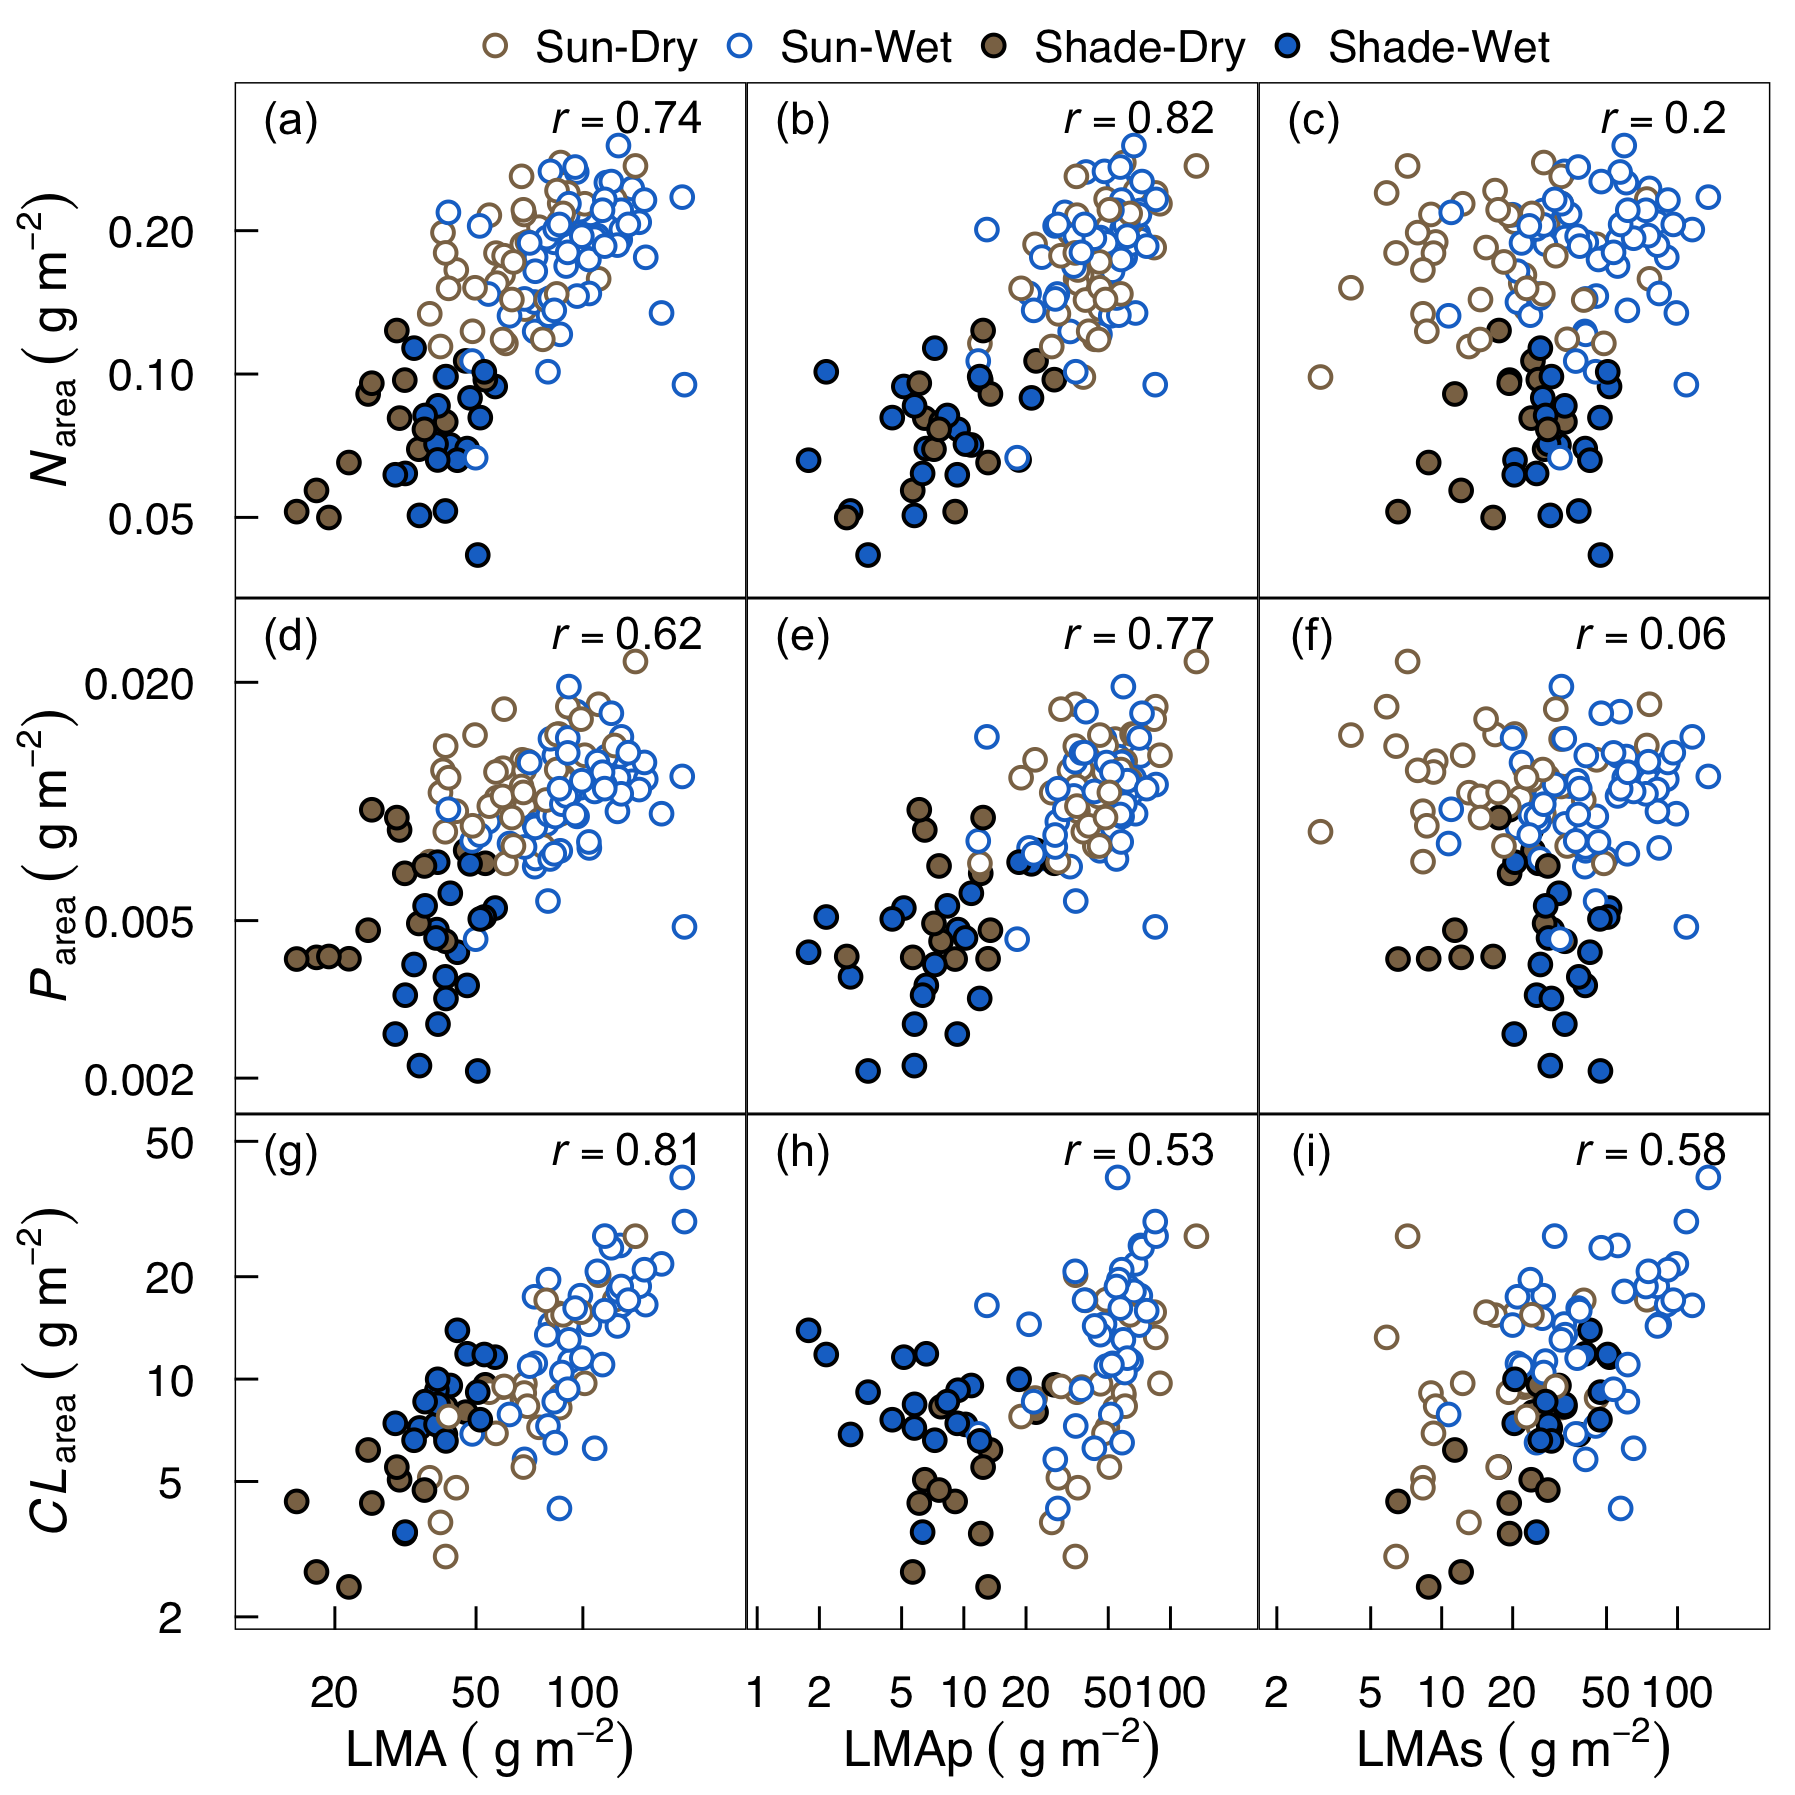
\includegraphics{../figs/PA_NPC.png}
\caption{Measured traits related to photosynthesis and metabolism traits (nitrogen and phosphorus per-unit leaf area; \emph{N}\textsubscript{area} and \emph{P}\textsubscript{area}) are strongly correlated with estimates (posterior medians) of the photosynthetic LMA component (LMAp), and a measured structural trait (cellulose per-unit leaf area; \emph{CL}\textsubscript{area}) is strongly correlated with estimates of the structural LMA component (LMAs) for the Panama dataset.
Note that sun and shade leaves align along a single relationship for \emph{CL}\textsubscript{area} vs.~LMAs, but not for \emph{CL}\textsubscript{area} vs.~LMA or LMAp. \emph{N}\textsubscript{area}, \emph{P}\textsubscript{area}, and \emph{CL}\textsubscript{area} data were not used to fit the models, and are presented here as independent support for the model results.
Analogous results were obtained for \emph{N}\textsubscript{area} and \emph{P}\textsubscript{area} vs.~LMAp for GLOPNET (Fig. S3).
Others details as in Fig.~\ref{fig:GLplt}.
Results for other LL models are reported in Table SX.}\label{fig:PA-NPC}
}
\DIFaddendFL \end{figure}

\end{document}
